\documentclass[fleqn,10pt]{wlscirep}
\usepackage{ctex}
\usepackage{graphicx}
\usepackage{amsmath}
\usepackage{multirow}
\usepackage{adjustbox}
\usepackage{subcaption}
\usepackage{pifont}
\usepackage{xr}
\usepackage{float}
\usepackage{nameref}
\usepackage{xcolor}
\usepackage{longtable}
\usepackage{booktabs}
\usepackage{array}
\usepackage{appendix}
\usepackage{hyperref}
\usepackage[nameinlink,noabbrev]{cleveref}
\usepackage{makecell}
\usepackage[table]{xcolor}
\usepackage{threeparttable}
\usepackage{diagbox}

\newcommand{\cmark}{\ding{51}}%
\newcommand{\xmark}{\ding{55}}%
\newcommand{\ph}[1]{\texttt{\textless #1\textgreater}}

\crefname{figure}{Fig.}{Figs.}
\crefname{table}{Table}{Tables}
\crefname{section}{Section}{Sections}
\crefname{appendix}{Supplementary}{Supplementary}

\title{Auditable agentic AI for evidence-grounded thyroid ultrasound diagnosis and reporting}
% An open clinician-interactive agentic AI system for thyroid ultrasound diagnosis and reporting

\author[1,$\dagger$]{Haifan Gong}
\author[1,$\dagger$]{Shiyu Chen}
\author[2,$\dagger$]{Bodong Wang}
\author[3,$\dagger$]{Yuqi Wang}
\author[4]{Shijie Wang}
\author[5]{Guoliang You}
\author[1]{Xinyu Xiong}
\author[6]{Haowei Wang}
\author[2]{Mingzhi Mao}
\author[4]{Dexing Kong}
\author[7,*]{Qinghua Liu}
\author[8,*]{Wei Lou}
\author[9,*]{Fei Chen}
\author[1,*]{Guanbin Li}

\affil[1]{School of Computer Science and Engineering, Sun Yat-sen University, Guangzhou, China}

\affil[2]{School of Software Engineering, Sun Yat-sen University, Zhuhai, China}

\affil[3]{Independent Researcher, Jersey City, NJ, USA}

\affil[4]{School of Mathematical Sciences, Zhejiang University, Hangzhou, China}

\affil[5]{Department of Radiology, Perelman School of Medicine, University of Pennsylvania, Philadelphia, PA, USA}

\affil[6]{Department of Pathology, Zhujiang Hospital, Southern Medical University, Guangzhou, China}

\affil[7]{Department of Health Management, Zhujiang Hospital, Southern Medical University, Guangzhou, China}

\affil[8]{College of Mathematical Medicine, Zhejiang Normal University, Jinhua, China}

\affil[9]{Department of Thyroid Surgery, Zhujiang Hospital, Southern Medical University, Guangzhou, China}

\affil[*]{\textbf{Corresponding authors:} Qinghua Liu~(\href{mailto:13760633321@163.com}{13760633321@163.com}), Wei Lou~(\href{mailto:louwei@zjnu.edu.cn}{louwei@zjnu.edu.cn}), Fei Chen~(\href{mailto:gzchenfei@126.com}{gzchenfei@126.com}), and Guanbin Li~(\href{mailto:liguanbin@mail.sysu.edu.cn}{liguanbin@mail.sysu.edu.cn})}
\affil[$\dagger$]{These authors contributed equally to this work}

\begin{abstract}
Thyroid ultrasound diagnosis requires coordinated lesion localization, measurement, risk stratification and reporting, yet most AI systems address these tasks in isolation and provide limited support for clinical review. We present ThyroidXAgent, a clinician-interactive agentic AI system that coordinates specialized diagnostic tools and stores their outputs as an auditable case-level evidence record. The system was developed using OpenThyroidDB, a multicentre, multitask resource integrating approximately 0.3 million ultrasound images and 24,000 paired reports, and was evaluated on 18,586 test images from seven cohorts and 8,721 test images from 35 centres in the private NHC-MISD-TUS cohort. Across the test cohorts, ThyroidXAgent achieved a mean Dice score of 87.01\% for nodule segmentation and a mean AUROC of 0.9057 for benign–malignant classification. The same workflow supported central lymph-node metastasis prediction and the classification of classic versus follicular-variant papillary thyroid carcinoma, with AUROCs of 0.856 and 0.783 on a patient-level hold-out set, respectively. For report generation, evidence-grounded assembly outperformed multimodal language-model baselines across three cohorts. ThyClinScore, a lesion-level clinical semantic metric introduced here, showed the strongest correlation with a location-aware language-model judge. ThyroidXAgent improved physician classification accuracy, increased report--annotation consistency from 70.3\% to 86.2\%, and reduced segmentation and reporting time by 35.9\% and 26.0\%, respectively. These findings support auditable, clinician-correctable agentic AI for thyroid ultrasound diagnosis and reporting.

\end{abstract}

\begin{document}
\flushbottom
\maketitle

\section{Introduction}

Thyroid ultrasound diagnosis depends on a sequence of lesion-level observations and clinical decisions \cite{Alexander2022Lancet,Grani2024NatRevEndocrinol}. A clinically useful examination localizes and measures thyroid nodules \cite{Alexander2022Lancet,Grani2024NatRevEndocrinol}, characterizes sonographic features \cite{Grani2024NatRevEndocrinol,Tessler2017ACRTIRADS,Hoang2018AJRInterobserver}, assigns risk using systems such as the Thyroid Imaging Reporting and Data System (TI-RADS) \cite{Tessler2017ACRTIRADS}, determines whether fine-needle aspiration is indicated \cite{Alexander2022Lancet,Tessler2017ACRTIRADS}, integrates cytology when available \cite{Cibas2017Bethesda} and communicates the findings in a structured report \cite{Grani2024NatRevEndocrinol,Tessler2017ACRTIRADS}. Each step introduces variability. Descriptors such as margins and echogenic foci \cite{Tessler2017ACRTIRADS,Hoang2018AJRInterobserver} show substantial reader dependence, and small changes in these features can alter biopsy or follow-up recommendations \cite{Tessler2017ACRTIRADS,Hoang2018AJRInterobserver}. These requirements make thyroid ultrasound a workflow-level problem for clinical AI \cite{Topol2019NatMedHighPerformance,Rajpurkar2022NatMedAIHealth}: useful systems must support prediction, preserve the evidence behind each step \cite{Chen2022HumanCenteredXAI} and allow clinicians to revise that evidence when needed \cite{Wekenborg2025RealWorldHAI,Giddings2024ClinicianPatientInteraction}.

Most thyroid ultrasound AI systems have focused on individual components of this workflow, including segmentation~\cite{gong2021multi,gong2023thyroid,sun2025clip}, classification~\cite{gong2022less,Peng2021LancetDigitalHealthThyNet,Chen2022RadiologyTIRADS,Yao2025NPJDigitMedThyGPT}, and report generation~\cite{li_ultrasound_2024,Tanno2025ClinicianVLM,li_towards_2025}. Multicenter systems \cite{Peng2021LancetDigitalHealthThyNet,Wang2024LancetDigitalHealthFNAB} and feature-aligned multimodal models \cite{Chen2022RadiologyTIRADS,Yao2025NPJDigitMedThyGPT,Tanno2025ClinicianVLM} have connected image predictions to risk descriptors \cite{Chen2022RadiologyTIRADS,Yao2025NPJDigitMedThyGPT} or management recommendations \cite{Peng2021LancetDigitalHealthThyNet,Yao2025NPJDigitMedThyGPT}. Recent studies have extended thyroid AI to fine-needle aspiration cytology \cite{Wang2024LancetDigitalHealthFNAB}, lateral lymph-node metastasis prediction \cite{Shen2025NatCommunLLNM} and rare thyroid cancer subtype classification \cite{Dai2025NatCommunThyroidSubtype}. Many systems still present their outputs as endpoints: a mask, probability, label or report-like text. The intermediate evidence that supports these outputs is often unavailable for clinical review \cite{Chen2022HumanCenteredXAI,Wekenborg2025RealWorldHAI}, correction \cite{Wekenborg2025RealWorldHAI,Giddings2024ClinicianPatientInteraction} or reuse across downstream tasks \cite{Chen2022HumanCenteredXAI,Tikhomirov2024LostCognitive,you2026learning}. This endpoint-oriented design makes it difficult to determine whether an AI result is supported by appropriate lesion localization, measurement, sonographic features and report statements.

This limitation reflects a broader challenge in medical AI. High-impact clinical AI studies increasingly emphasize workflow integration \cite{Vasey2022NatMedDECIDEAI,Wekenborg2025RealWorldHAI,dreyer2025mechanistic}, human-AI collaboration \cite{Topol2019NatMedHighPerformance,Patel2019HumanMachinePartnership,Leibig2022RadiologistsAI,Yu2024AIAssistanceRadiologists,Chen2024WorkloadCollaboration,Everett2026ToolTeammate,Strong2026HumanAICollaboration}, and evidence beyond retrospective performance \cite{Wiens2019NatMedDoNoHarm,Topol2019NatMedHighPerformance,Rajpurkar2022NatMedAIHealth,Vasey2022NatMedDECIDEAI}. The cognitive consequences of AI-supported clinical work \cite{Tikhomirov2024LostCognitive}, clinician interaction with algorithmic recommendations \cite{Giddings2024ClinicianPatientInteraction} and the transition of AI from a tool to a clinical teammate \cite{Zou2025LancetAgenticTeammates,Everett2026ToolTeammate} have also become central considerations. Generalist medical AI \cite{Moor2023NatureGMAI,Kohane2024InjectingAI,Katz2024GPTResidents,Zhou2026NEJMAIMedVersa} and multimodal foundation models \cite{Moor2023NatureGMAI,Zhou2026NEJMAIMedVersa,Tu2025ConversationalAI,McDuff2025DifferentialDiagnosis,deltadahl2025deep,pontikos2025next} extend this ambition to flexible inputs and outputs across tasks. For thyroid ultrasound, however, generality must be connected to specialty-specific requirements: lesion-level measurement \cite{Alexander2022Lancet,Tessler2017ACRTIRADS}, sonographic feature attribution \cite{Tessler2017ACRTIRADS,Chen2022RadiologyTIRADS}, anatomical context \cite{Grani2024NatRevEndocrinol}, guideline-aligned management \cite{Alexander2022Lancet,Tessler2017ACRTIRADS,Peng2021LancetDigitalHealthThyNet} and auditable reporting \cite{Chen2022HumanCenteredXAI,Tanno2025ClinicianVLM,Wekenborg2025RealWorldHAI}. We therefore treat the case-level evidence record, rather than a single prediction endpoint, as the central object of AI assistance.

Agent-based workflows \cite{Qiu2024NatMachIntellAgenticSystems,Zou2025LancetAgenticTeammates,Moritz2025NatBMECoordinatedAgents,Ferber2026AutonomousAgents,Collaco2026AgenticAIReview,kong2025ai} provide one way to implement this evidence-centred formulation. In this setting, the agent's role is coordination rather than direct image interpretation \cite{Qiu2024NatMachIntellAgenticSystems,Zou2025LancetAgenticTeammates,Moritz2025NatBMECoordinatedAgents}: it acts as a workflow controller that plans case-specific analysis \cite{wang_plan-and-solve_2023,Schmidgall2026AgentClinic,Liu2026AgentBenchmark}, routes inputs to specialized tools \cite{yao_react:_2022,Moritz2025NatBMECoordinatedAgents,Ferber2026AutonomousAgents}, maintains intermediate state \cite{Tian2026AutonomousWorkflow} and exposes structured evidence for human review \cite{Chen2022HumanCenteredXAI,Wekenborg2025RealWorldHAI,Zou2025LancetAgenticTeammates}. Medical-agent benchmarks increasingly emphasize these capabilities in interactive settings \cite{Jiang2025NEJMAIMedAgentBench,Schmidgall2026AgentClinic,Liu2026AgentBenchmark} that require retrieval, action execution and workflow-level reasoning \cite{yao_react:_2022,Jiang2025NEJMAIMedAgentBench,Tian2026AutonomousWorkflow}. For thyroid ultrasound, the relevant evidence objects include images, lesion masks and measurements \cite{gong2021multi,gong2023thyroid,zhang2025tn5000}, radiomic descriptors and risk estimates \cite{van2017computational,Chen2022RadiologyTIRADS,Yao2025NPJDigitMedThyGPT}, report clauses \cite{rebuff_data2text_2020,li_ultrasound_2024,Tanno2025ClinicianVLM}, uncertainty signals \cite{farquhar2024detecting} and clinician corrections \cite{Yu2024AIAssistanceRadiologists,Chen2024WorkloadCollaboration,Wekenborg2025RealWorldHAI}. The agent is therefore useful insofar as it can coordinate these objects into an auditable clinical workflow.

Here we present ThyroidXAgent, a clinician-interactive agentic system that reframes thyroid ultrasound AI around an auditable case-level evidence record rather than a collection of isolated prediction endpoints. Instead of directly interpreting ultrasound images with a general-purpose multimodal model, ThyroidXAgent acts as a workflow controller that plans case-specific analyses, routes inputs to specialized tools and maintains structured intermediate evidence, including lesion masks, measurements, class probabilities, radiomic descriptors, uncertainty signals and report clauses. These evidence objects remain inspectable and editable by clinicians, and corrections can be propagated to subsequent analysis and reporting steps. We evaluate this formulation across nodule segmentation, benign-malignant classification, malignant-lesion stratification and case-level report generation on 18,586 test images from seven OpenThyroidDB cohorts, 8,721 test images from the private NHC-MISD-TUS multicentre set (35 contributing sites), and complementary report-generation cohorts, together with clinician reader studies. We further introduce ThyClinScore, a lesion-level semantic metric that evaluates whether generated reports preserve clinically relevant evidence rather than surface-level wording alone. ThyroidXAgent produced more clinically consistent reports and reduced clinician workload while retaining an editable evidence trace. Together, these results establish evidence-centred orchestration as an alternative to both standalone predictive models and unconstrained end-to-end medical agents.


\begin{figure}[p]
    \centering
    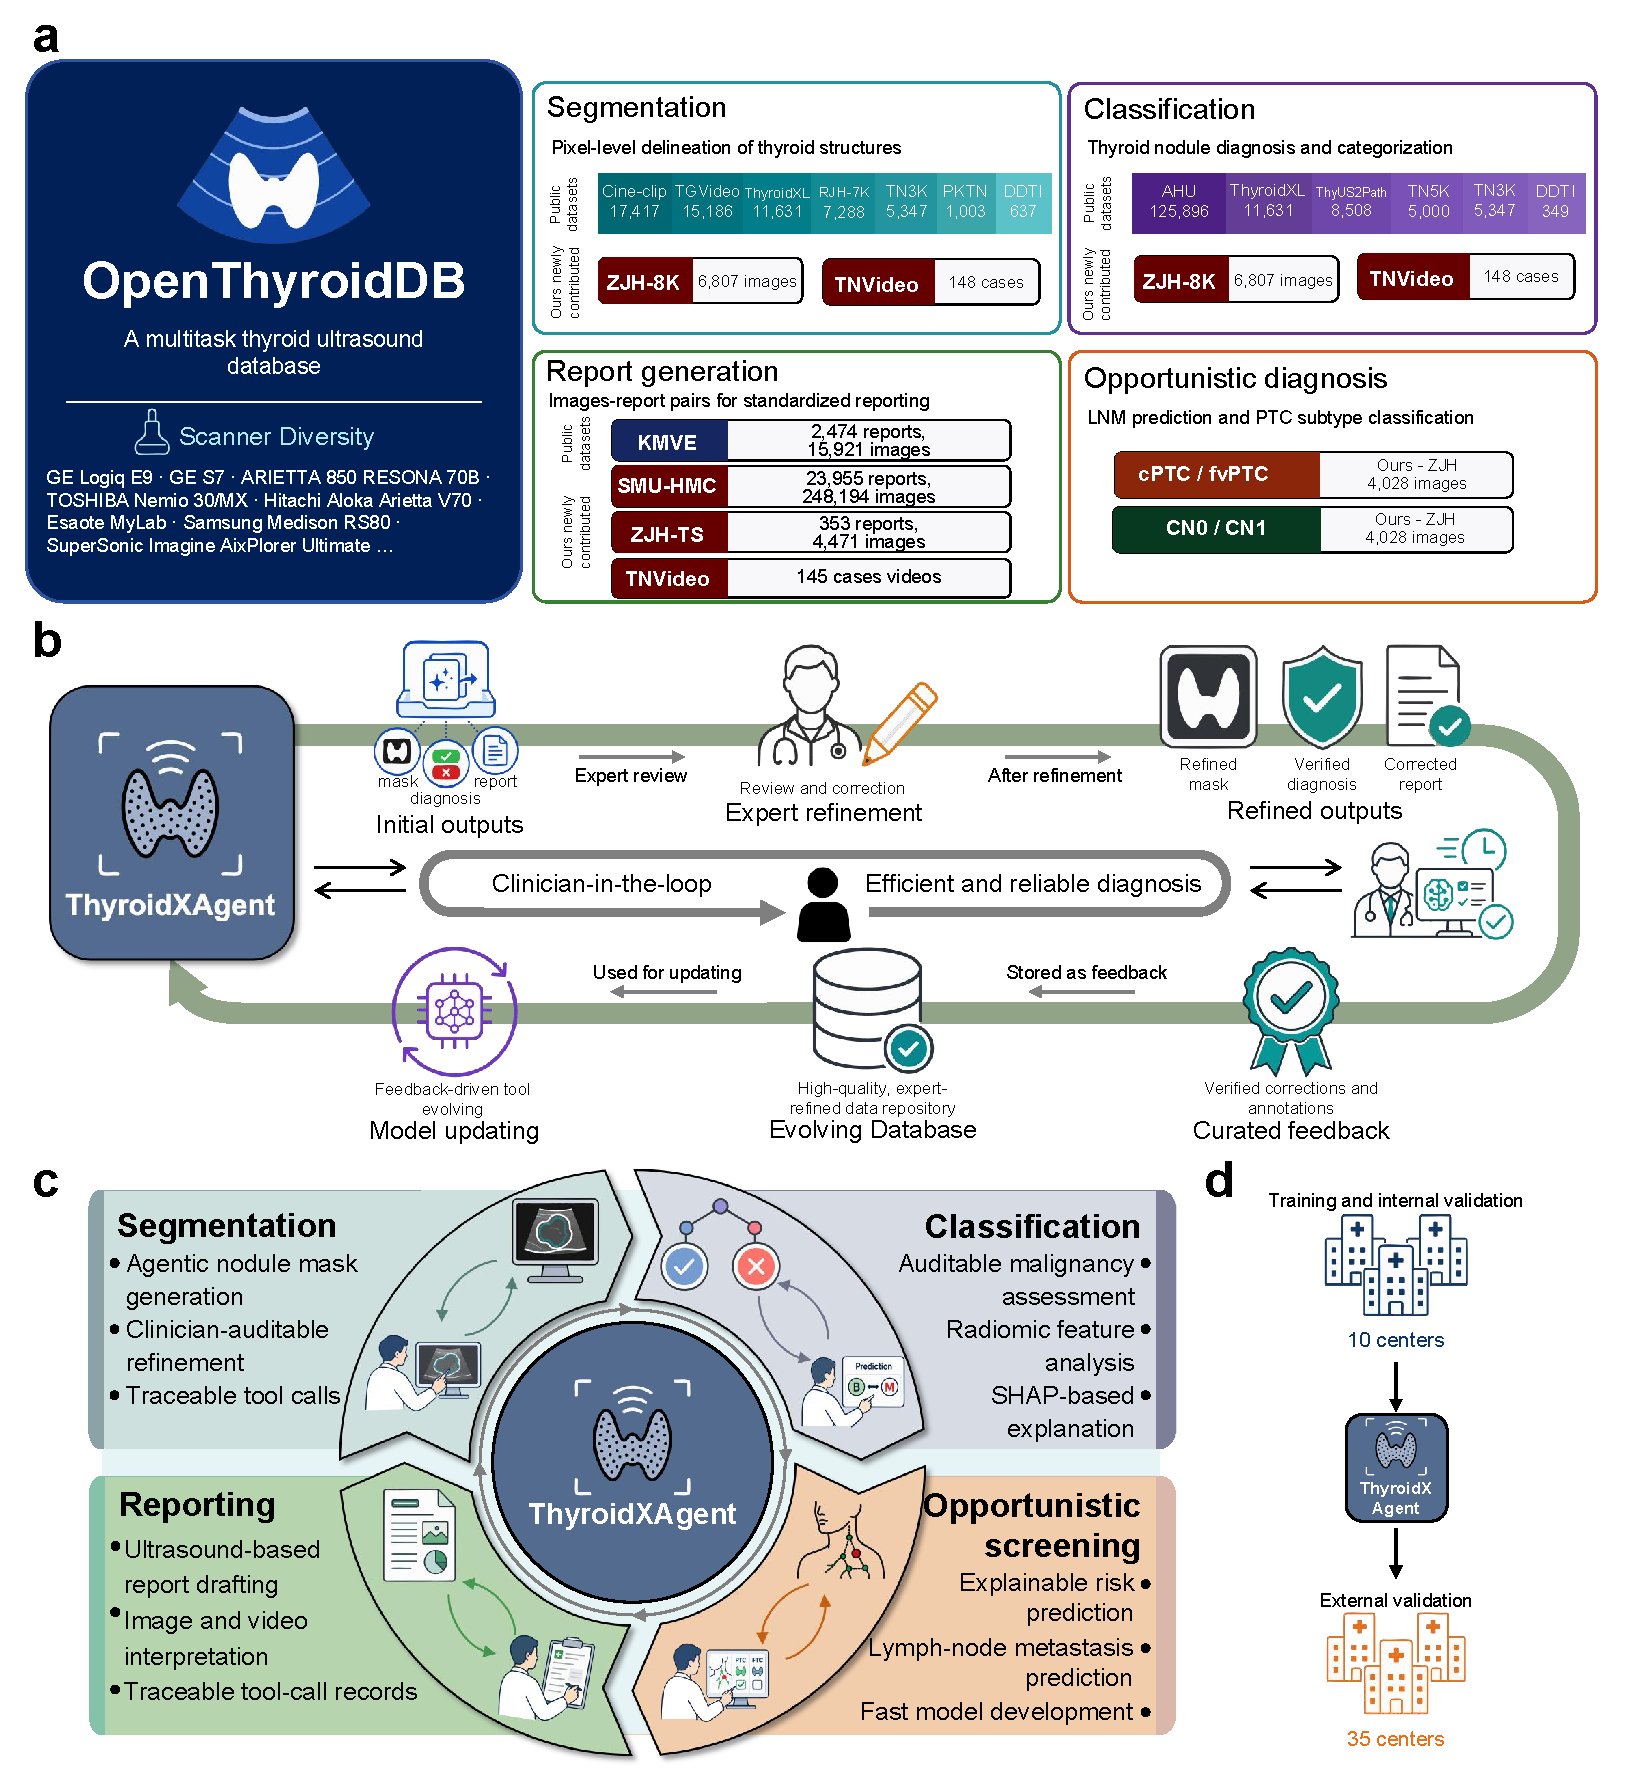
\includegraphics[width=0.9\textwidth]{imgs/Introduction3.pdf}
    \caption{Multicenter thyroid ultrasound data and the ThyroidXAgent evidence workflow. \textbf{a}, OpenThyroidDB integrates curated public thyroid ultrasound resources and institutionally governed clinical cohorts into a full-spectrum resource for segmentation, benign-malignant classification, report generation and malignant-lesion stratification across diverse scanners and acquisition settings. \textbf{b}, The clinician-feedback workflow stores AI-generated masks, predictions, report clauses and clinician corrections as case-level evidence, allowing intermediate outputs to be reviewed, revised and reused in later steps. \textbf{c}, ThyroidXAgent acts as a workflow controller for four evidence-producing workflows: expert-refined nodule segmentation, clinician-verified malignancy classification, evidence-grounded structured reporting, and advanced diagnosis for central lymph-node metastasis assessment and PTC subtype analysis. \textbf{d}, Multicenter validation design, with model development/internal validation followed by independent external validation.}


    \label{fig:introduction_overview}
\end{figure}


\begin{figure}[htbp]
    \centering
    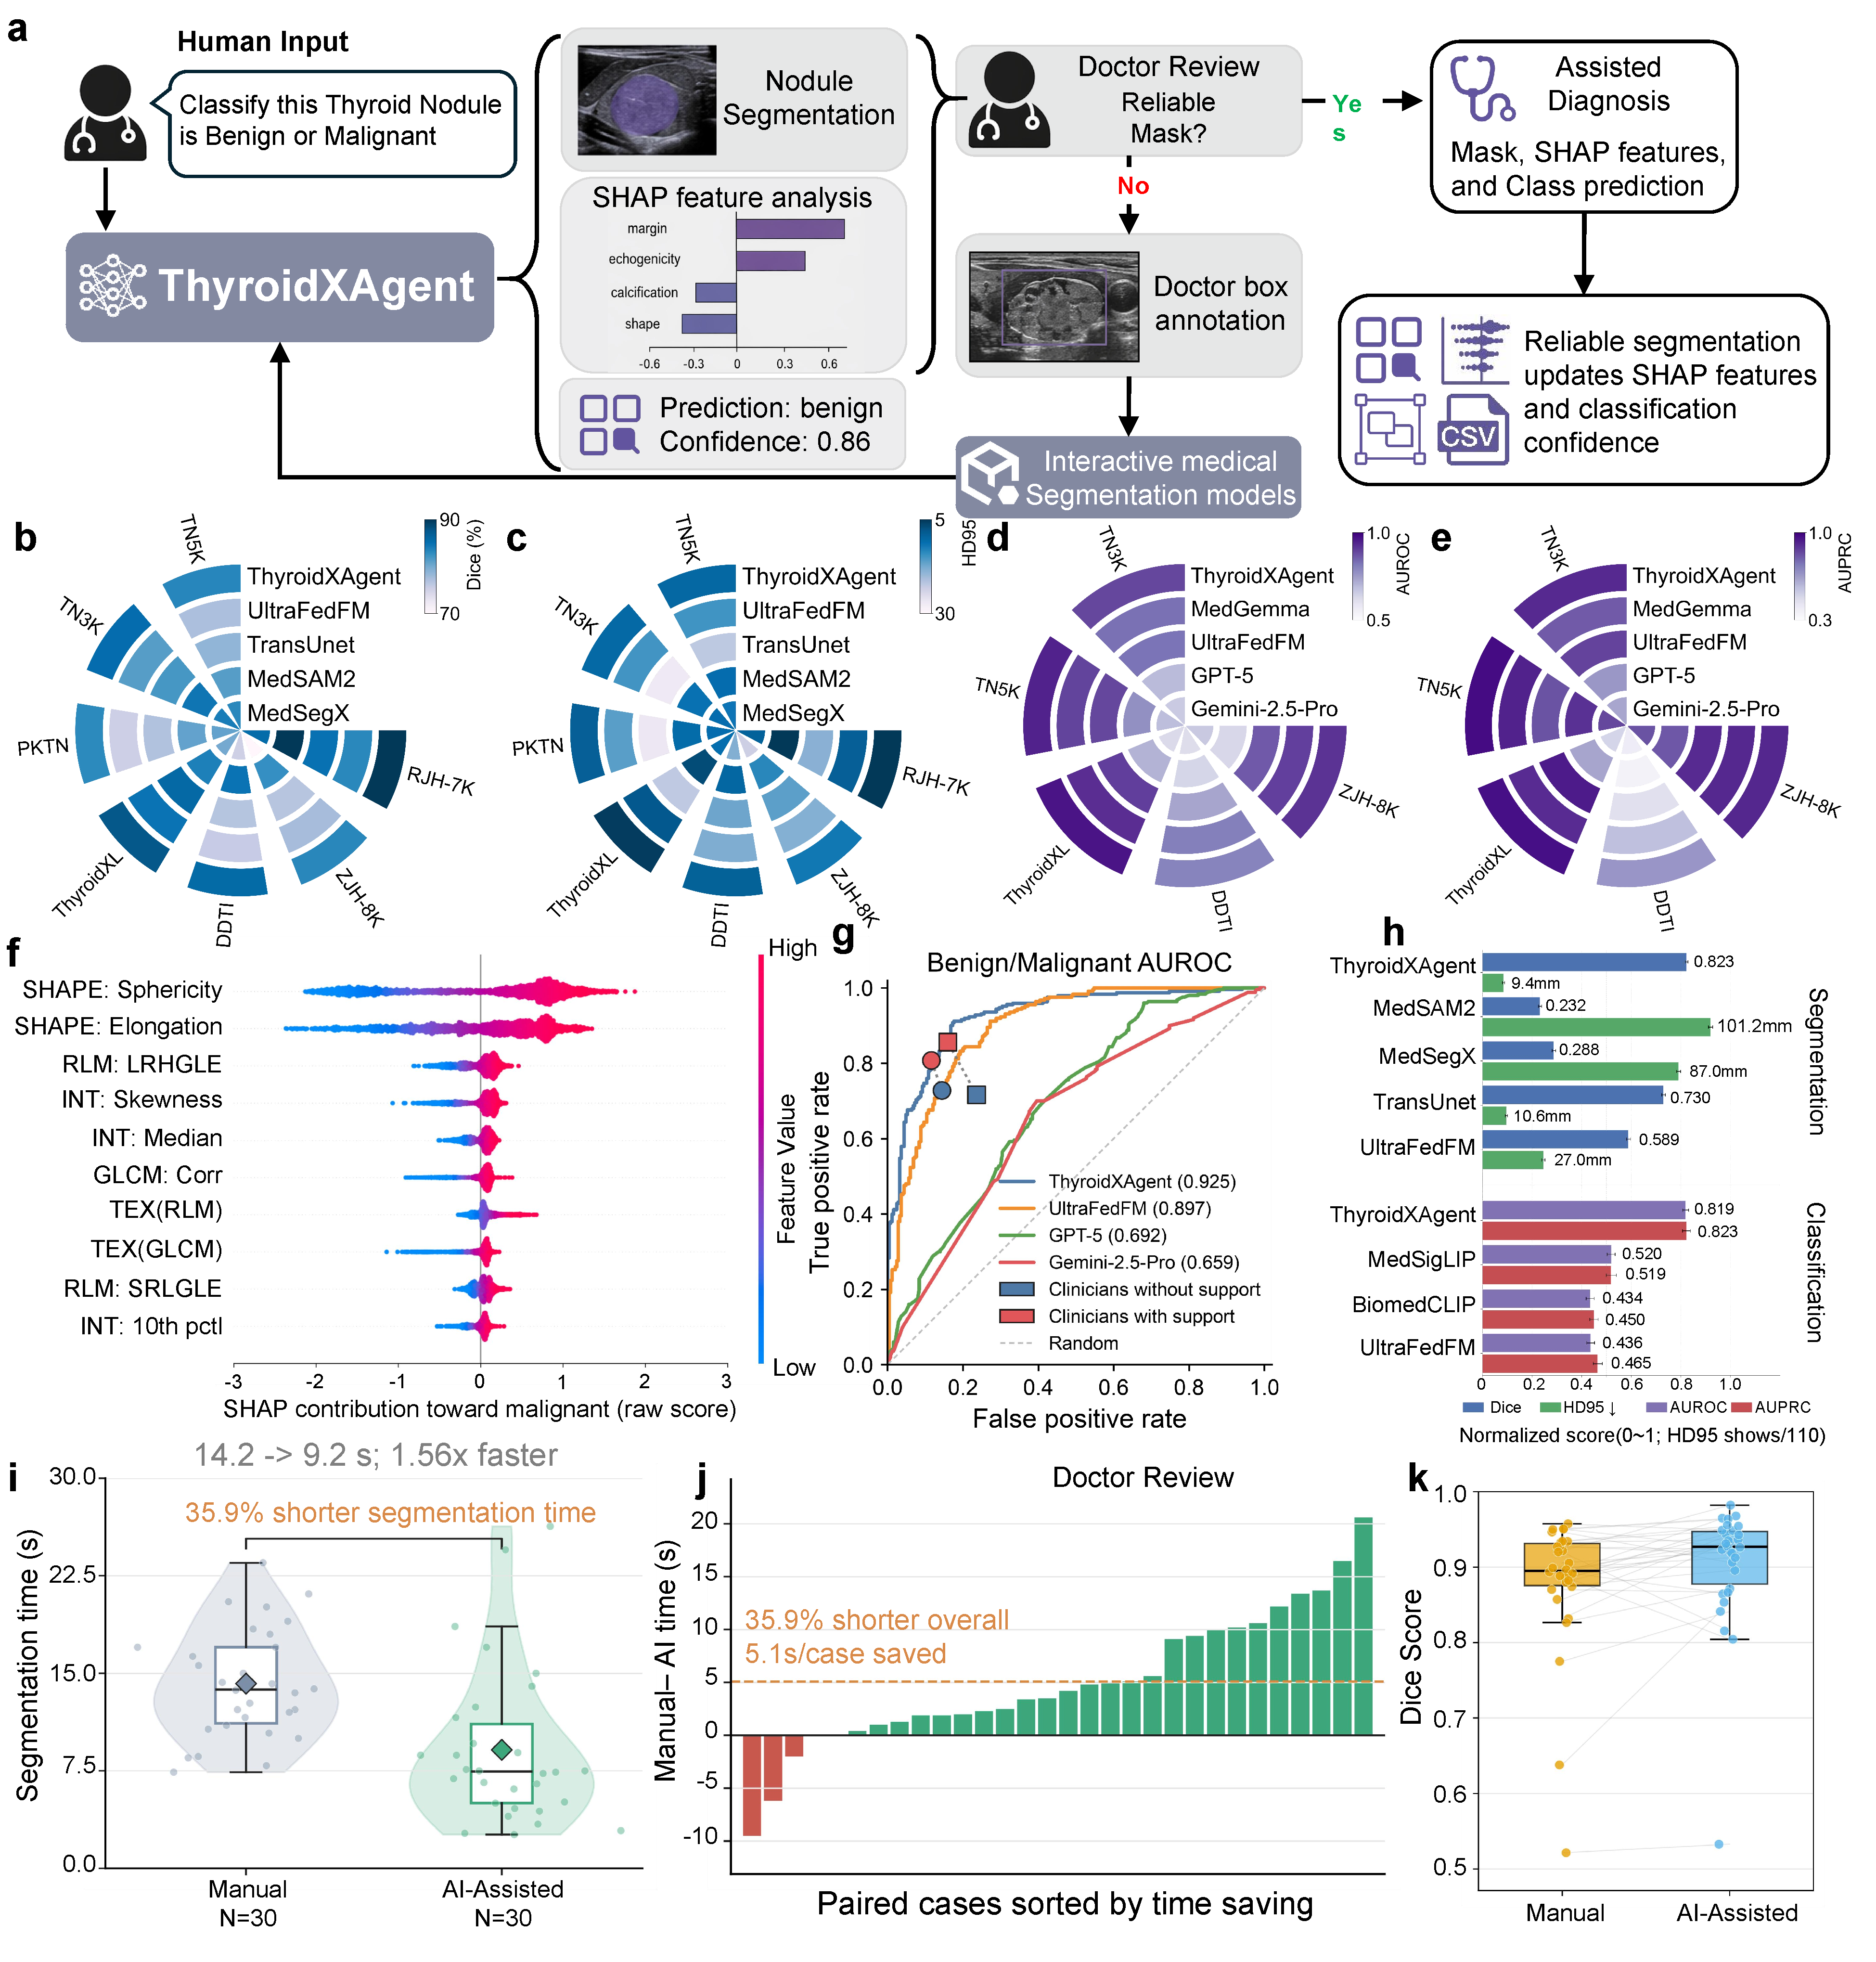
\includegraphics[width=0.9\textwidth]{imgs/ThyroidXAgent_SegCls_performance.pdf}
    \caption{Agent-routed evidence for thyroid nodule segmentation, benign-malignant classification and clinician review. \textbf{a}, Interactive review workflow: clinicians assess the predicted nodule mask, accept the classification if the mask is reliable, or refine it through box annotation and interactive segmentation; SHAP-based feature attributions are then recomputed from the corrected mask. \textbf{b-e}, Segmentation and classification performance across heterogeneous thyroid ultrasound benchmarks, evaluated using Dice, HD95, AUROC and AUPRC. \textbf{f}, Cohort-level SHAP beeswarm analysis for benign-malignant classification. \textbf{g}, ROC curves on the 500-image physician comparison set, showing ThyroidXAgent, representative AI baselines and clinician operating points before and after ThyroidXAgent support; both clinicians improved with evidence support. \textbf{h}, Pooled performance on the NHC-MISD-TUS private external test set across nine models and four metrics: nodule Dice, HD95, binary AUROC and AUPRC. Bars show point estimates with 95\% CIs, and the dashed line indicates the classification chance level of 0.5. \textbf{i}, Segmentation time for manual and AI-assisted workflows. \textbf{j}, Ranked within-case time savings. \textbf{k}, Paired Dice distributions showing preserved segmentation quality with improved efficiency.}
    \label{fig:ThyroidXAgent_SegCls_performance}
\end{figure}

\section{Results}
\subsection{ThyroidXAgent organizes thyroid ultrasound diagnosis as an auditable case-level evidence workflow}

We developed ThyroidXAgent to organize thyroid ultrasound diagnosis as a case-level evidence workflow (Fig.~\ref{fig:introduction_overview}). For each examination, the agent routes the case through tool-callable steps, including nodule segmentation, measurement, benign-malignant classification, radiomics extraction, malignant-lesion stratification and report generation. The workflow stores tool outputs in a shared evidence record that can be inspected, corrected and reused across downstream tasks.

OpenThyroidDB provides the multicenter data resource underlying this workflow-level formulation. The segmentation and classification analyses included seven cohorts from six clinical centres across China, Vietnam and Colombia, acquired on at least eight ultrasound platforms (Supplementary Table~\ref{tab:dataset_summary}). Four cohorts served as internal training data. TN3K~\cite{gong2021multi}, collected at Zhujiang Hospital, Southern Medical University, Guangzhou, comprised 4,633 training, 100 validation and 614 test images acquired on GE Logiq E9, ARIETTA 850 and RESONA 70B scanners. TN5K~\cite{zhang2025tn5000}, from the Cancer Hospital, Chinese Academy of Medical Sciences, Beijing, comprised 3,500 training, 500 validation and 1,000 test images acquired on GE Logiq E9 and GE S7 scanners with 5-12 or 8-15~MHz probes. ThyroidXL~\cite{duong2025thyroidxl}, from the Vietnam National Hospital of Endocrinology, Hanoi, comprised 9,441 training, 100 validation and 2,090 test images acquired on a Hitachi Aloka Arietta V70 scanner. PKTN~\cite{sun2025clip}, from Peking University First Hospital, Beijing, comprised 703 training, 150 validation and 150 test images; the acquisition device was not disclosed. Three cohorts served as test sets: DDTI and RJH-7K as independent external cohorts, and ZJH-8K as a same-centre institutional hold-out cohort from the hospital that contributed TN3K. DDTI~\cite{pedraza2015open}, from IDIME, Bogot\'{a}, Colombia, contributed 637 images (637 for segmentation, 349 of which also carry benign-malignant classification labels) acquired on TOSHIBA Nemio 30 and Nemio MX scanners with a 12~MHz probe. RJH-7K~\cite{shusharina2021segmentation}, from Ruijin Hospital, Shanghai Jiao Tong University School of Medicine, Shanghai, contributed 7,288 segmentation-only images acquired on multiple scanners whose models were not specified. ZJH-8K, collected at Zhujiang Hospital, Southern Medical University, Guangzhou, contributed 6,807 test images (1,068 patients) used for both segmentation and classification; the acquisition device was not disclosed. Overall, the segmentation and classification benchmark comprised 37{,}713 images (18{,}277 training, 850 validation, 18{,}586 test) from seven cohorts spanning six centres.


The report-generation analyses included four cohorts from three centres. SMU-HMC comprised 23,955 reports from 21,954 patients, with 248,194 associated ultrasound images. A patient-level held-out set of 400 patients, comprising 5,984 images, was reserved for internal testing. After excluding all examinations from these internally held-out patients, the remaining SMU-HMC cohort was used to develop the relevant component models, and 7,147 quality-controlled reports were selected to construct the retrieval template library. The KMVE analysis cohort~\cite{li_ultrasound_2024} comprised 2,457 cases and 4,914 image assignments, partitioned according to the original dataset split into 1,719 training, 246 validation and 492 test cases; its training partition was additionally used for template-library construction. External evaluation included two complementary cohorts. ZJH-TS provided an independent external-centre test set of 150 reports selected from the original collection of 353 reports, after excluding reports dominated by postoperative findings. TNVideo provided an independently assembled case-level cohort for the external reader study, comprising 151 ultrasound videos, of which 145 had annotation-derived case labels. Overall, the report-generation analyses comprised four cohorts from three centres, including an internal SMU-HMC test set, an independent external-centre test set and an external reader-study cohort.

For malignant-lesion stratification, we used malignant primary-lesion images from ZJH-8K, which also served as the same-centre hold-out test set for segmentation and classification. A total of 4,028 images from 647 patients were split by patient into a development set (3,227 images, 517 patients), evaluated with five-fold cross-validation, and a hold-out test set (801 images, 130 patients) shared by both tasks. The tasks were central lymph-node metastasis (LNM) prediction, labelled CN0 or CN1 from postoperative pathology, and classification of classic versus follicular-variant papillary thyroid carcinoma (PTC).

Collectively, these resources cover heterogeneous acquisition settings, file formats, annotation types and clinical tasks, including nodule segmentation, benign-malignant classification, report generation and advanced malignant-lesion analysis (Fig.~\ref{fig:introduction_overview}a and Supplementary Table~\ref{tab:dataset_comparison}). Using this resource, ThyroidXAgent coordinates four evidence-producing workflow branches: expert-refined nodule segmentation, clinician-verified malignancy classification, expert-edited report generation and advanced diagnosis for central lymph-node metastasis and PTC subtype analysis (Fig.~\ref{fig:introduction_overview}b,c). Each branch contributes structured evidence to the same case-level record, including masks, measurements, class probabilities, radiomic descriptors, feature attributions, uncertainty signals and report clauses. This design allows intermediate outputs to be reused across tasks. A corrected mask can support radiomics extraction, a malignancy estimate can inform the report impression, and structured report evidence can be reviewed and edited rather than accepted as opaque text.

The resulting workflow makes auditability a property of the diagnostic process rather than a post hoc explanation attached to a final answer. Clinicians can inspect generated masks, correct segmentation errors, review SHAP- or Grad-CAM-based explanations, edit report statements and return corrected outputs to the evidence store. The subsequent results evaluate this formulation across automatic image analysis, clinician correction, malignant-lesion stratification, clinical semantic report scoring and evidence-grounded report assembly.

\subsection{Agent-routed evidence improves cross-dataset segmentation and classification}

We first evaluated the two image-analysis tasks that anchor the downstream workflow: nodule segmentation and benign-malignant classification. For each case, ThyroidXAgent collected candidate masks and class probabilities from DINOv3-based experts, selected or fused outputs using case-level quality signals, extracted radiomic features from the selected lesion mask and stored confidence, disagreement and tabular predictions as structured evidence (Supplementary Fig.~\ref{fig:ThyroidXAgent_for_seg_and_cls}). This design tests whether tool routing and evidence consolidation improve robustness across heterogeneous ultrasound datasets, where dataset bias remains a major source of performance degradation~\cite{liu2024decade}.

On seven segmentation test sets, including the independent DDTI and RJH-7K cohorts and the same-centre ZJH-8K hold-out cohort, ThyroidXAgent achieved a mean Dice coefficient of 87.01\% and a mean 95th-percentile Hausdorff distance (HD95) of 7.46~mm (unweighted means across test sets; Fig.~\ref{fig:ThyroidXAgent_SegCls_performance}b,c and Supplementary Table~\ref{tab:seg_performance}). It obtained the highest Dice score and the lowest HD95 on all seven test sets, indicating improved boundary robustness across heterogeneous acquisition conditions. The strongest baseline, MedSAM2~\cite{ma2025medsam2}, achieved a mean Dice of 85.13\%. UltraFedFM~\cite{jiang2025pretraining}, a medical imaging foundation model, reached 79.22\%.

For benign-malignant classification, ThyroidXAgent achieved a mean AUROC of 0.9057 and a mean AUPRC of 0.8923 across five test sets, including the independent DDTI cohort and the same-centre ZJH-8K hold-out cohort (unweighted means; Fig.~\ref{fig:ThyroidXAgent_SegCls_performance}d,e and Supplementary Table~\ref{tab:cls_performance}). At the patient level, AUROC was 0.951 on ZJH-8K (1,068 patients) and 0.980 on ThyroidXL (739 patients) (Supplementary Table~\ref{tab:patient_level}). Specialized image models showed weaker cross-dataset consistency; for example, RepViT~\cite{wang2023repvit} reached AUROC of 0.777 on ThyroidXL but 0.556 on TN3K. General-purpose vision-language models~\cite{dong2022survey} also underperformed; GPT-5~\cite{openai2025gpt5systemcard} reached AUROC of 0.632-0.774 across test sets, and Gemini-2.5-Pro~\cite{comanici_gemini_2025} reached 0.616-0.687 (Supplementary Table~\ref{tab:cls_performance}). These results support a division of labour in which domain-specific image and radiomics tools generate the evidence, while the agent routes and consolidates tool outputs. We further validated on NHC-MISD-TUS, an independent private multicentre external test set of 8,721 gland-segmentation test images from 35 contributing sites (6,384 nodule-segmentation and 4,999 benign--malignant classification images where labels were available; Fig.~\ref{fig:ThyroidXAgent_SegCls_performance}h and Supplementary Tables~\ref{tab:nodule_dice}-\ref{tab:binary_auprc}). ThyroidXAgent led on both nodule segmentation (Dice 82.31\%, HD95 9.41~mm) and binary classification (AUROC 0.819, AUPRC 0.823). These pooled estimates were higher than the centre-level macro averages (nodule Dice 81.64\% over 33 centres and AUROC 0.754 over 32 centres), and between-centre heterogeneity was high ($I^2$ = 99.0\% for both; Supplementary Table~\ref{tab:nhc_heterogeneity}). By contrast, MedSAM2 and MedSegX failed on segmentation (Dice <0.3), and zero-shot vision-language baselines (BiomedCLIP~\cite{zhang2024biomedclip}, MedSigLIP~\cite{sellergren2025medgemma}) performed at or below chance on classification. GPT-5 and Gemini-2.5-Pro could not be evaluated on this private intranet dataset.


Beyond prediction accuracy, we examined whether the structured evidence provided interpretable signals for clinician review. Cohort-level SHAP profiles~\cite{lundberg2017unified} showed that morphology-related radiomic descriptors, especially Sphericity and Elongation, dominated benign-malignant classification, whereas texture and intensity features contributed complementary information (Fig.~\ref{fig:ThyroidXAgent_SegCls_performance}f). Representative cases confirmed that accurate segmentation produced SHAP attributions and Grad-CAM maps aligned with visible nodule characteristics, whereas poor segmentation degraded these explanations (Supplementary Fig.~\ref{fig:BM_cases}).

To assess whether this evidence supports clinician decision-making, we conducted a blinded 500-image physician comparison (Fig.~\ref{fig:ThyroidXAgent_SegCls_performance}g). ThyroidXAgent achieved AUROC of 0.9256 and AUPRC of 0.9250. In the same comparison, UltraFedFM~\cite{jiang2025pretraining} reached AUROC of 0.880, GPT-5~\cite{openai2025gpt5systemcard} 0.660 and Gemini-2.5-Pro~\cite{comanici_gemini_2025} 0.619. When clinicians were provided with ThyroidXAgent's structured evidence, including SHAP-based feature attributions and nodule segmentation boundaries, both clinicians improved across all metrics. For clinician 1, accuracy rose from 79.2\% to 84.6\% (+5.4\%), precision from 83.5\% to 87.5\%, recall from 72.8\% to 80.8\%, specificity from 85.6\% to 88.4\%, and F1 from 0.778 to 0.840, while the false-positive rate fell from 14.4\% to 11.6\%. Clinician 2 improved more markedly: accuracy from 74.0\% to 84.8\% (+10.8\%), precision from 75.2\% to 84.3\%, recall from 71.6\% to 85.6\%, specificity from 76.4\% to 84.0\%, and F1 from 0.734 to 0.849, with the false-positive rate decreasing from 23.6\% to 16.0\%; clinician 2 thereby narrowly surpassed clinician 1 as the higher-performing reader.

\subsection{Clinician correction reduces segmentation time while preserving quality}

The same evidence representation supported clinician-interactive segmentation review. Clinicians inspected predicted masks, corrected segmentation errors when needed and returned the refined masks to the case-level evidence store. SHAP-based feature attributions were then recomputed using the corrected mask, allowing downstream classification evidence to reflect clinician refinement (Fig.~\ref{fig:ThyroidXAgent_SegCls_performance}a).

AI assistance reduced mean segmentation time from 14.21~s to 9.11~s per image, a 1.6-fold speedup, while preserving segmentation quality (Fig.~\ref{fig:ThyroidXAgent_SegCls_performance}i-k). AI-assisted Dice (0.903) matched or exceeded manual Dice (0.879) in approximately two-thirds of paired cases. These results indicate that the intermediate evidence layer can reduce repetitive annotation work while keeping the segmentation boundary available for clinician correction.


\begin{figure}[htbp]
    \centering
    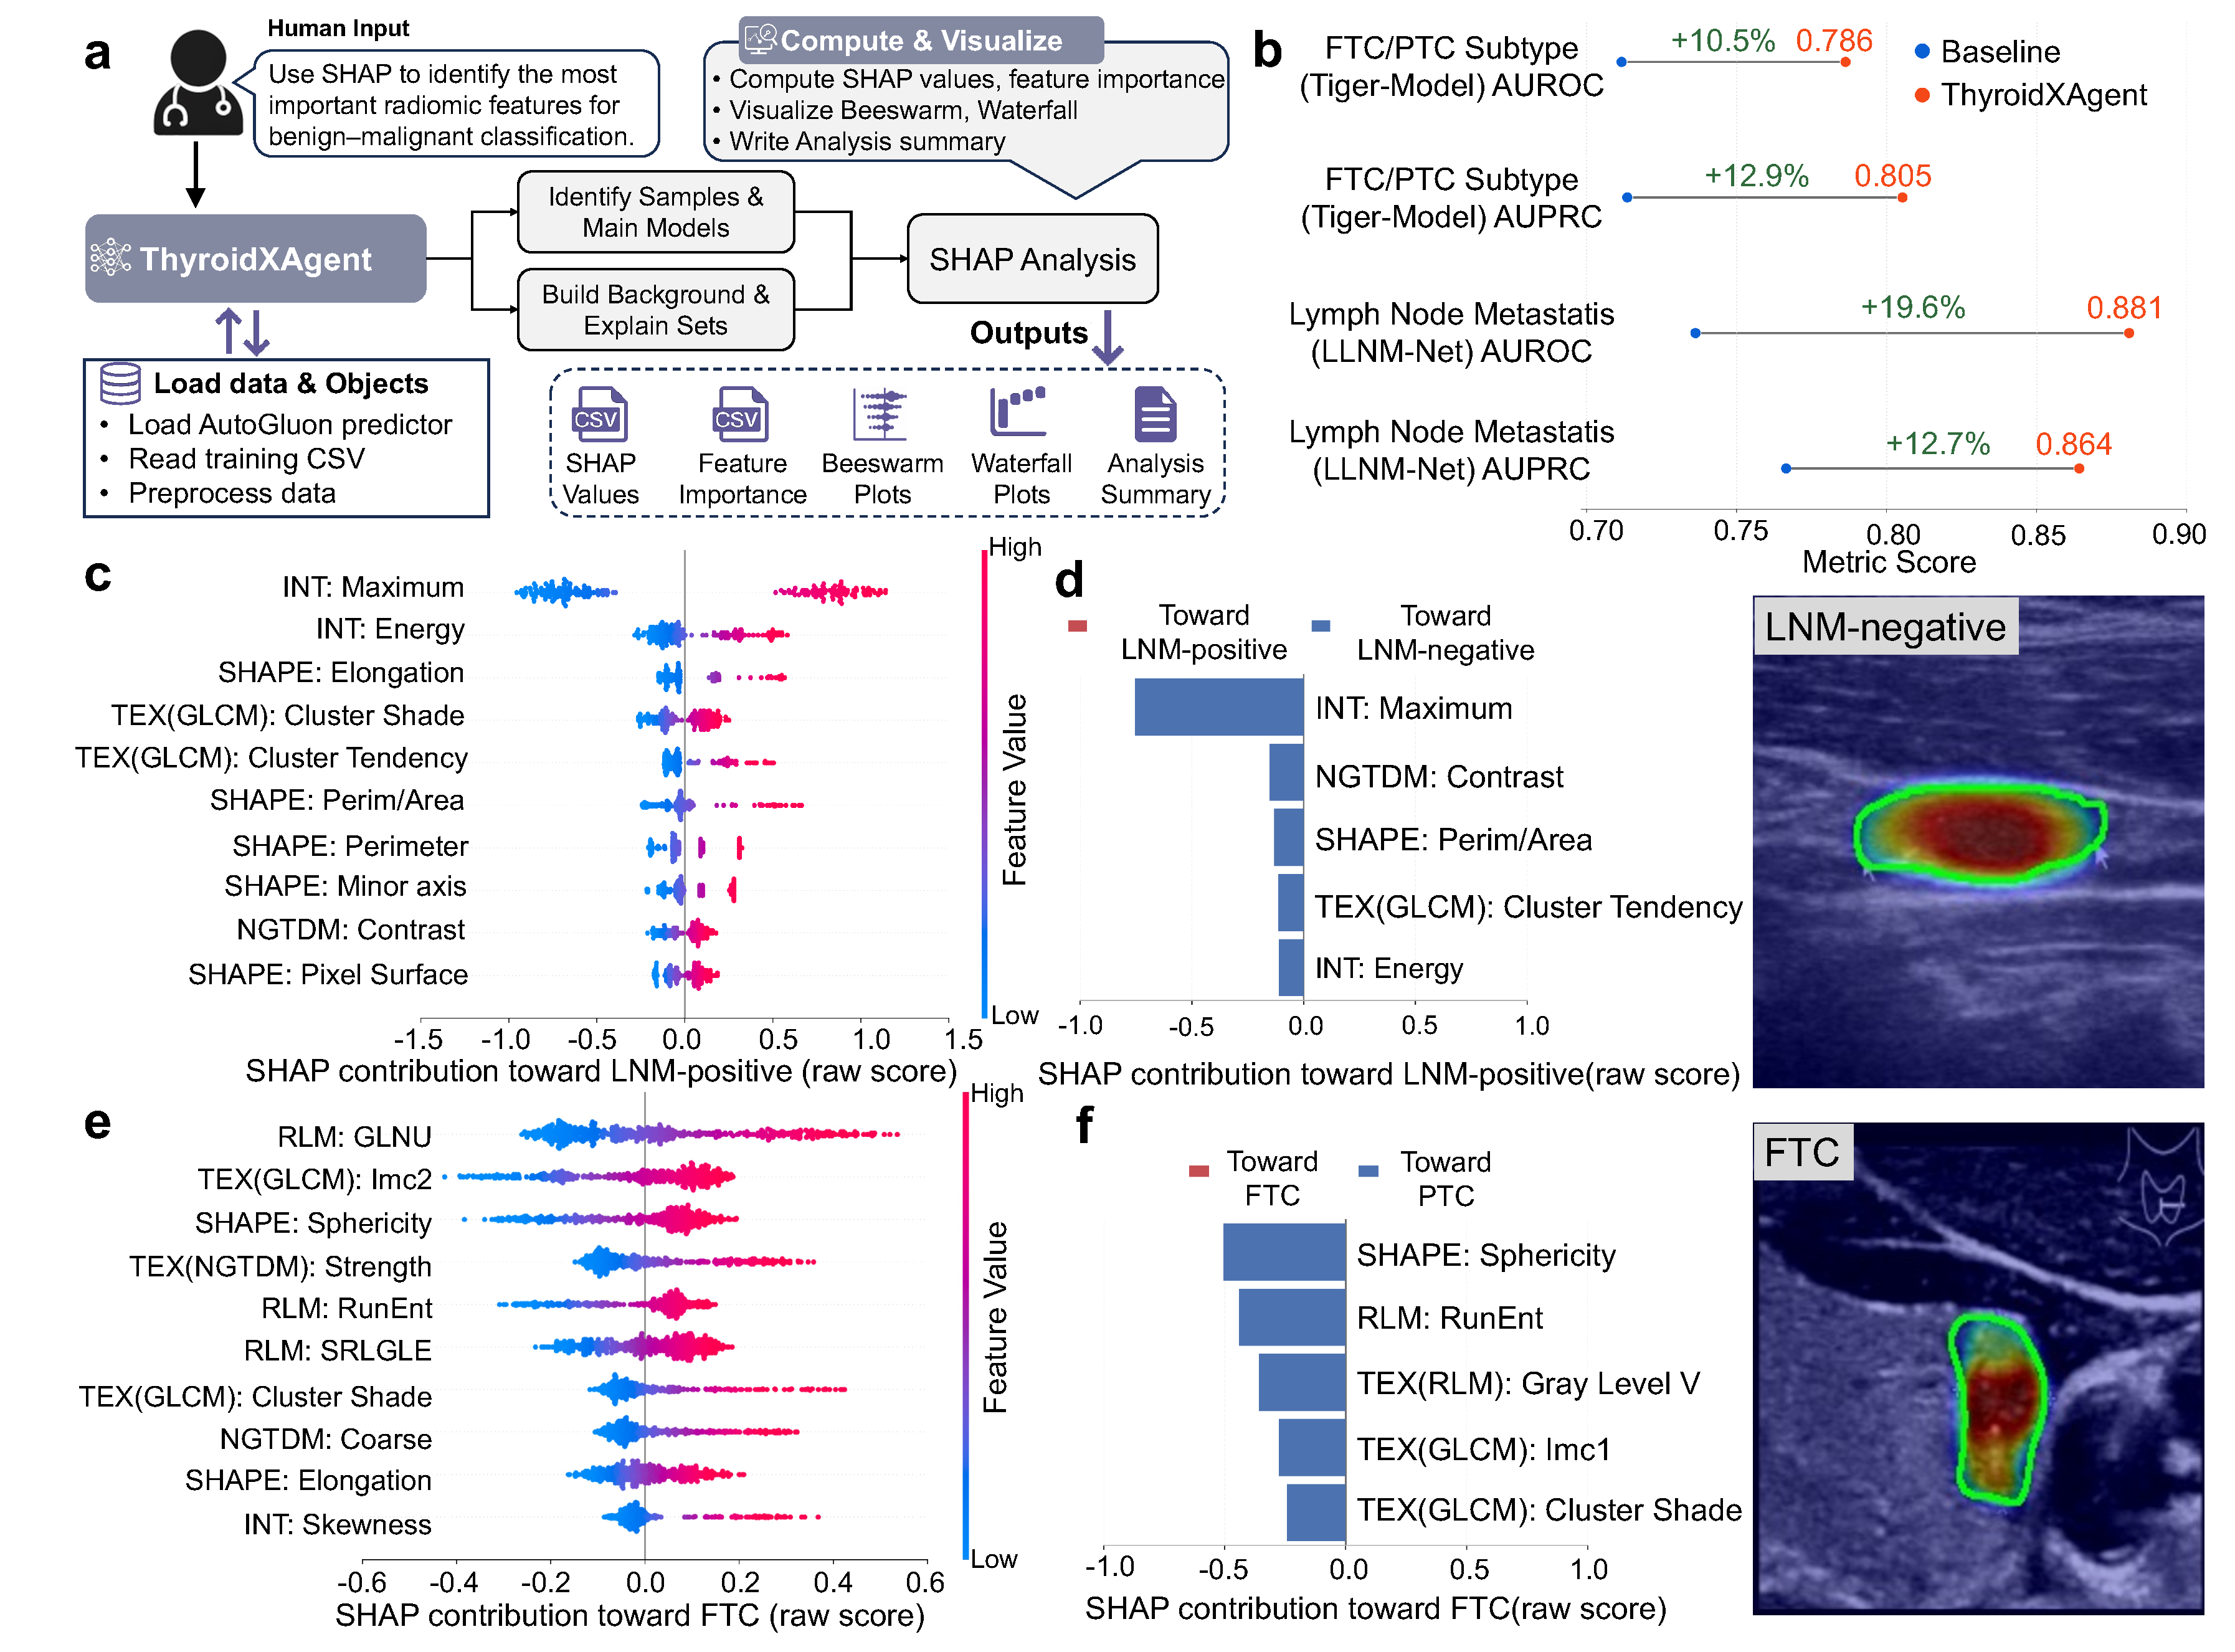
\includegraphics[width=\textwidth]{imgs/Malignant_Image_tasks.pdf}
    \caption{Shared ThyroidXAgent tools support malignant-lesion stratification with task-specific radiomic attributions. \textbf{a}, Workflow for SHAP-based interpretation of malignant-lesion tasks. \textbf{b}, Performance comparison between ThyroidXAgent and the corresponding specialist baselines for PTC subtype classification and central lymph-node metastasis prediction on the hold-out test set, reported as AUROC and AUPRC; percentages denote the relative improvement of ThyroidXAgent over each baseline. \textbf{c,d}, Global and representative local SHAP analyses for central lymph-node metastasis prediction. \textbf{e,f}, Global and representative local SHAP analyses for PTC subtype classification, showing stronger contributions from texture heterogeneity and shape descriptors.}

    \label{fig:ThyroidXAgent_Malignant_Image_tasks}
\end{figure}

\subsection{Shared agent tools generate task-specific evidence for malignant-lesion stratification}

We next tested whether the shared ThyroidXAgent tools could be redirected to clinically distinct malignant-lesion stratification tasks after the primary thyroid nodule assessment. Central lymph-node metastasis (LNM) prediction informs surgical planning, whereas distinguishing classic from follicular-variant papillary thyroid carcinoma (PTC) informs treatment strategy and follow-up. In a conventional development pipeline, each task would require a separate workflow for preprocessing, feature extraction, prediction, interpretation and reporting. In ThyroidXAgent, the segmentation, radiomics extraction, tabular classification and routing logic were reused, with task-specific classifier fine-tuning and task instructions changed.

This reuse enabled rapid adaptation to new clinical questions while preserving the same evidence structure. On the patient-level hold-out test set (130 patients), ThyroidXAgent achieved AUROC of 0.856 for LNM prediction and 0.783 for PTC subtype classification (Fig.~\ref{fig:ThyroidXAgent_Malignant_Image_tasks}b and Supplementary Table~\ref{tab:Malignant_images_tasks_performance}), outperforming the specialist baselines LLNM-Net~\cite{Shen2025NatCommunLLNM} (0.812) for LNM and Tiger-Model~\cite{Dai2025NatCommunThyroidSubtype} (0.754) for PTC subtype. Five-fold cross-validation on the development set gave AUROCs of 0.880 and 0.809, respectively.

The attribution profiles changed with the clinical task (Fig.~\ref{fig:ThyroidXAgent_Malignant_Image_tasks}a,c-f). LNM prediction relied more on lesion position and size features, including distance to the thyroid capsule and lesion area. PTC subtype classification relied more on texture heterogeneity and shape descriptors. These task-dependent attribution patterns indicate that ThyroidXAgent generated radiomic evidence according to the requested clinical question, rather than simply reusing the benign-malignant decision rule.
\begin{figure}[htbp]
    \centering
    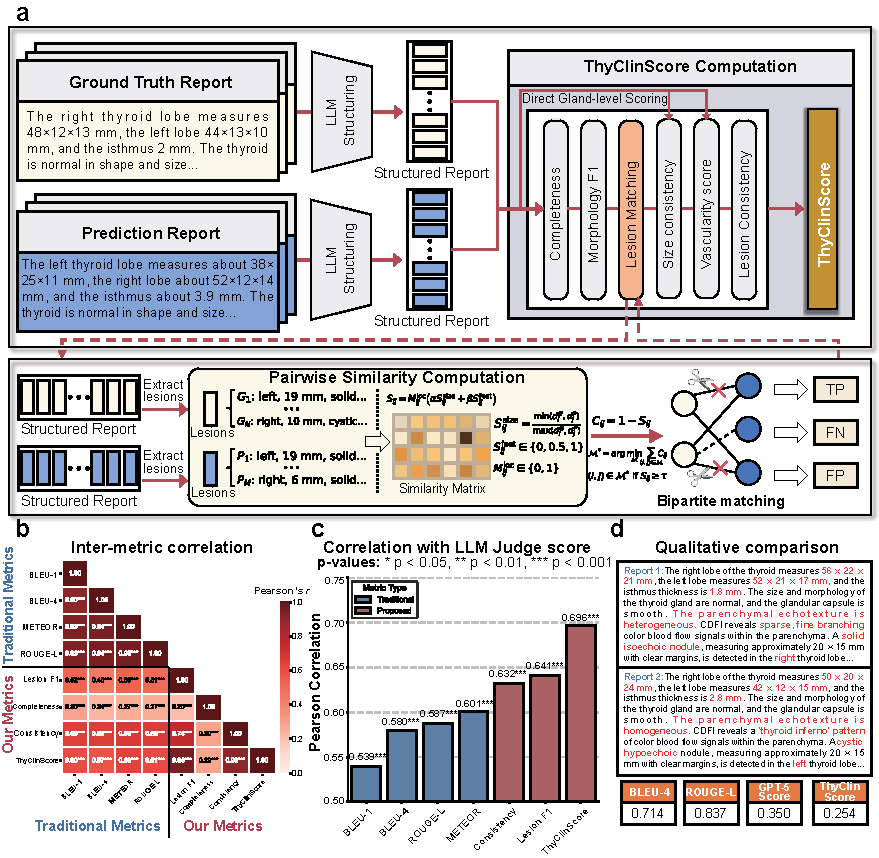
\includegraphics[width=\textwidth]{imgs/ThyClinScore2.pdf}
    \caption{ThyClinScore for clinical semantic evaluation of thyroid ultrasound reports. \textbf{a}, ThyClinScore first structures the ground-truth and predicted reports into lesion-level entries, matches corresponding lesions, and scores clinically relevant attributes, including size, vascularity, morphology, lesion-level F1 and completeness. \textbf{b}, Pearson correlation matrix comparing conventional natural-language generation metrics with clinical semantic metrics. Overlap-based metrics were highly correlated with one another, whereas the clinical semantic metrics captured complementary report-quality dimensions. \textbf{c}, Pearson correlations between each metric and a location-aware LLM judge. ThyClinScore showed the strongest correlation among the evaluated metrics; asterisks denote statistical significance (* \(p<0.05\), ** \(p<0.01\), *** \(p<0.001\)). \textbf{d}, Qualitative comparison showing that reports with similar wording overlap can differ in clinically important lesion attributes, which is reflected by ThyClinScore.}
    \label{fig:thyclinscore}
\end{figure}

\begin{figure}[htbp]
    \centering
    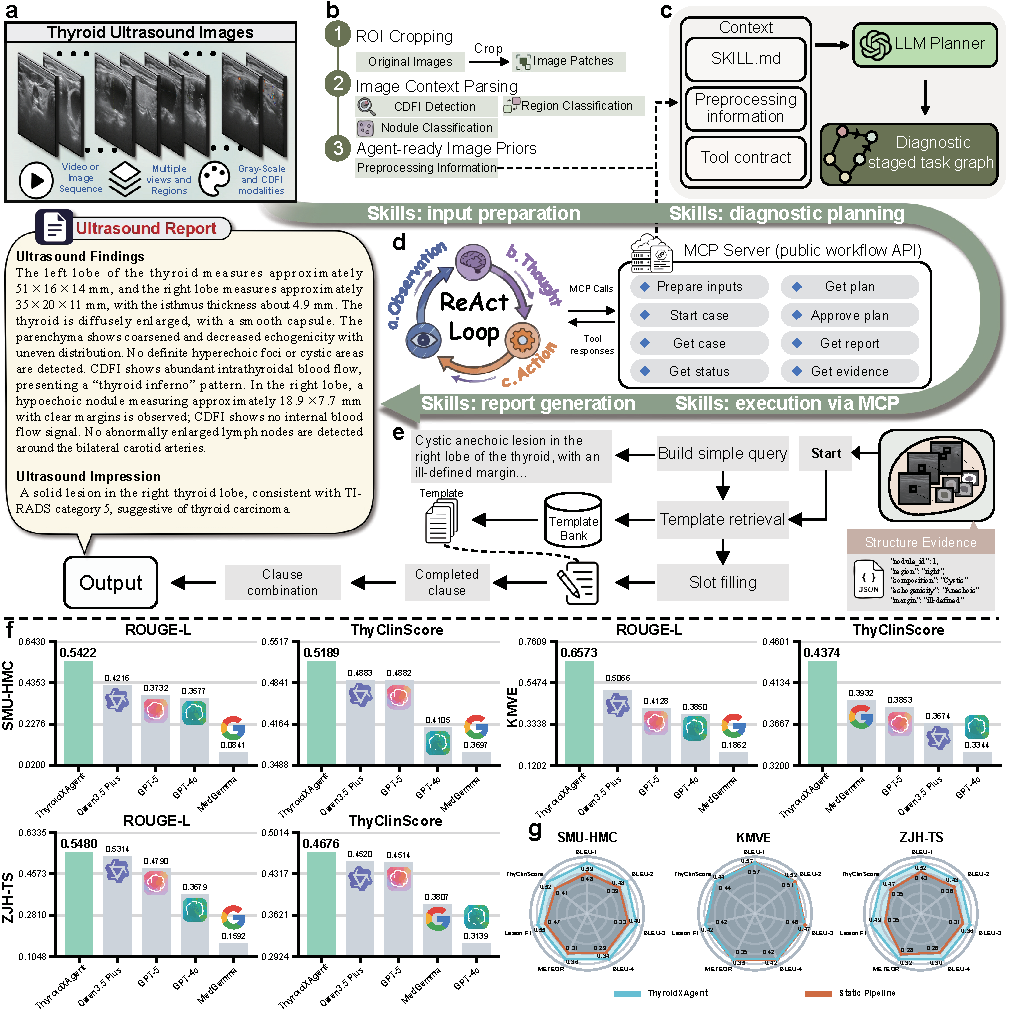
\includegraphics[width=\textwidth]{imgs/ReportGen3.pdf}
    \caption[Evidence-grounded report assembly in ThyroidXAgent]{
    Evidence-grounded report assembly in ThyroidXAgent. \textbf{a}, Case-level thyroid ultrasound input, including video or image sequences, multiple views and anatomical regions, and greyscale and CDFI modalities. \textbf{b}, Input-preparation skills crop regions of interest, parse image context, detect CDFI information, classify nodules and anatomical regions, and convert the resulting preprocessing outputs into agent-ready image priors. \textbf{c}, Diagnostic planning combines the skill instructions, preprocessing information and tool contract with an LLM planner to generate a staged diagnostic task graph. \textbf{d}, A ReAct-style execution loop observes intermediate evidence, reasons over the next step and calls tools through an MCP server that exposes the public workflow API, including case initialization, plan approval, status checking, evidence retrieval and report generation. \textbf{e}, Structured evidence is transformed into report text through query construction, template retrieval, slot filling and clause combination, so that report clauses remain linked to measurements, lesion descriptors, risk estimates and other case-level evidence. \textbf{f}, Report-generation performance comparison on SMU-HMC, KMVE and ZJH-TS. \textbf{g}, Radar plots comparing ThyroidXAgent with the static pipeline across lexical and clinical semantic metrics.
    }
    \label{fig:thyroidxagent_report_generation}
\end{figure}

\subsection{ThyClinScore captures lesion-level report errors missed by overlap metrics}

We then addressed the evaluation of thyroid ultrasound reports. Conventional natural-language generation metrics, such as BLEU~\cite{papineni_bleu:_2001}, ROUGE~\cite{lin_rouge_2004}, and METEOR~\cite{lavie_meteor:_2007}, primarily reward surface overlap and can miss clinically important disagreements in lesion location, size, vascularity, morphology or impression. We therefore developed ThyClinScore, a clinical semantic metric that structures ground-truth and generated reports, matches lesion entries and scores clinically relevant attributes (Fig.~\ref{fig:thyclinscore}a).

ThyClinScore captured report-quality dimensions that were complementary to wording overlap. Overlap-based metrics were strongly correlated with one another, whereas the clinical semantic metrics captured distinct lesion-level and feature-level information (Fig.~\ref{fig:thyclinscore}b). Using a Pearson correlation-based evaluation approach similar to that of Li \textit{et al.}~\cite{li_towards_2025}, ThyClinScore showed the strongest correlation with a location-aware LLM judge among the evaluated metrics (Pearson's \(r=0.696\), \(p<0.001\); Fig.~\ref{fig:thyclinscore}c). Qualitative examples further show that reports with similar wording overlap can differ in clinically important attributes, which is reflected by the ThyClinScore components (Fig.~\ref{fig:thyclinscore}d).

We further validated ThyClinScore against blinded clinician ratings. Two clinicians independently rated 270 reports of 90 cases (30 cases per test set; the ThyroidXAgent report and two baseline reports per case) against the reference report on clinical accuracy, factual consistency, completeness, readability and clinical usability, blinded to the system. ThyClinScore correlated with the clinical-accuracy rating on all three test sets (Spearman's \(\rho=0.437\), 0.560 and 0.464 on SMU-HMC, KMVE and ZJH-TS, respectively; all 95\% CIs excluded zero). Inter-rater agreement (ICC(2,1)) was between 0.54 and 0.79 for clinical accuracy, factual consistency and clinical usability, and lower for completeness (0.33 to 0.57) and readability (0.08 to 0.25; Supplementary Table~\ref{tab:thyclinscore_clinician}). Across 120 configurations of the weights and thresholds of ThyClinScore, ThyroidXAgent had the highest mean ThyClinScore in all 120 configurations on SMU-HMC, in 110 on KMVE and in 117 on ZJH-TS.


\subsection{Evidence-grounded report assembly improves reporting consistency and efficiency}

For report generation, ThyroidXAgent converted the case-level evidence record into structured report text. The agent first used multi-view and multimodal thyroid ultrasound inputs to construct image priors, invoked diagnostic tools through planning and execution, and then assembled report clauses from structured facts using BM25 template retrieval, slot filling and clause combination (Fig.~\ref{fig:thyroidxagent_report_generation}a-g). This design links report statements to intermediate evidence, including gland measurements, nodule location, lesion size, sonographic descriptors, vascularity, lymph-node findings and diagnostic impressions, rather than generating unconstrained free text. The report-generation workflow was packaged as a reusable skill and exposed to external agents through a Workflow MCP server. This interface provided high-level case operations, including input preparation, case initiation, plan review, approval, report retrieval and evidence retrieval, while low-level model calls remained internal to the workflow. Auxiliary tool performance is summarized in Supplementary Table~\ref{tab:auxiliary_tools}. Clinicians can review the structured evidence, edit generated statements and return corrected report content to the case-level evidence store. We also audited the failure modes of the planner-executor workflow in 450 runs (150 cases from the three test sets, each run three times; 2,347 tool calls). Four tool calls (0.17\%) were invalid, three planned tasks (0.13\%) lacked support in the case images, no tool was called repeatedly apart from one retry after a malformed tool name, and all runs were completed. The main failure modes were ordering errors and omitted steps: in 40 of 320 fusion calls, nodule fusion preceded pixel-spacing estimation, which left five nodule descriptions without a size in four SMU-HMC and ZJH-TS runs, and in one run a segmented nodule was not reported because fusion was missing from the plan.

On conventional natural-language generation metrics, ThyroidXAgent achieved the strongest overall performance across SMU-HMC, KMVE~\cite{li_ultrasound_2024} and ZJH-TS (Fig.~\ref{fig:thyroidxagent_report_generation}f and Supplementary Table~\ref{tab:report_generation_nlg_ci}). The comparison methods generated reports directly from a subset of the case images (in KMVE, all methods received the same two images per case), whereas ThyroidXAgent derived structured evidence from all images with specialized tools and assembled the report from templates (Methods); these comparisons therefore evaluate evidence-grounded report assembly as a whole rather than language-generation ability. On SMU-HMC, ThyroidXAgent ranked first on all reported overlap metrics, with BLEU-1, BLEU-4 and ROUGE$_L$ of 0.5924, 0.3381 and 0.5422, respectively. On KMVE, ThyroidXAgent ranked first on all reported overlap metrics, with BLEU-1 of 0.5675, BLEU-4 of 0.4183, METEOR of 0.3505 and ROUGE$_L$ of 0.6573. On ZJH-TS, ThyroidXAgent achieved the highest BLEU-4 and ROUGE$_L$ values, reaching 0.3018 and 0.5480, respectively, whereas Qwen3.5 Plus had the highest BLEU-1, BLEU-2 and METEOR (0.5379, 0.4297 and 0.3456 versus 0.5233, 0.4296 and 0.3191).

We further compared the adaptive tool-routing workflow with a fixed rule-based tool-calling pipeline (Fig.~\ref{fig:thyroidxagent_report_generation}g and Supplementary Table~\ref{tab:static_rule_controller_radar_metrics}). On SMU-HMC and ZJH-TS, ThyroidXAgent produced larger multi-metric profiles than the static pipeline, and ThyClinScore increased from 0.4129 to 0.5189 and from 0.3528 to 0.4676, respectively. On KMVE, the two had the same ThyClinScore (0.4374), because KMVE reports focus on qualitative descriptions of the gland and nodules with measurements masked, so that a few tools suffice to generate them (Supplementary Table~\ref{tab:report_generation_tool_ablation}).

Clinical semantic evaluation showed that the reports retained clinically relevant information beyond wording similarity (Fig.~\ref{fig:thyclinscore} and Supplementary Table~\ref{tab:report_generation_clinical_ci}). ThyroidXAgent achieved the highest ThyClinScore on SMU-HMC (0.5189), KMVE (0.4374) and ZJH-TS (0.4676). It also achieved the highest lesion-level F1 and report completeness on SMU-HMC and ZJH-TS. Notably, other baselines led on some submetrics. In the blinded clinician rating, ThyroidXAgent reports scored higher than the baseline reports of the same case in factual consistency (2.94 versus 2.46), readability (4.52 versus 4.08) and clinical usability (2.88 versus 2.41) on a scale of 1 to 5. By test set, the differences were clear on SMU-HMC and ZJH-TS, mainly because in cases without nodules in the reference report, the baseline reports often described nodules that were not in the reference, whereas the ThyroidXAgent reports rarely did. On KMVE, the differences were small (0.09 to 0.22). Together with the metric-correlation analysis (Fig.~\ref{fig:thyclinscore}b,c), these results indicate that clinical semantic scoring captures report-quality information not represented by conventional overlap metrics.

We next assessed human-AI cooperation in a cross-over reader study. Two physicians wrote reports for 145 thyroid ultrasound videos under manual and AI-assisted workflows, with each case evaluated in both workflows by different physicians to reduce memory bias (Fig.~\ref{fig:reader_study}a). In the 145 cases with annotation-derived case labels, the annotation consistency of the reports increased with AI assistance from 70.3\% to 86.2\%, with increases in both the benign and the malignant subsets (Fig.~\ref{fig:reader_study}c); by physician, it increased from 72.6\% to 84.7\% and from 68.1\% to 87.7\%. The paired difference over the 145 cases was 15.9 percentage points (95\% CI 9.7 to 22.1; McNemar's test, \(p<0.001\)), and the same difference was estimated with the physician as a covariate. AI assistance reduced mean reporting time from 2.5 to 1.8 min per case, a 26.0\% reduction; the reduction was 13.0\% for one reader and 36.8\% for the other (Fig.~\ref{fig:reader_study}d,e). A representative malignant case shows that the structured evidence supported statements on gland morphology, nodule location, measurements, sonographic features and diagnostic impression, while leaving partially correct or incorrect statements available for clinician review (Fig.~\ref{fig:reader_study}b and Supplementary Fig.~\ref{fig:RG_CaseReview}).

Finally, we conducted an additional reader study with safety rules that mark the sentences of an AI draft requiring physician review (Supplementary Table~\ref{tab:safety_rules}), in which two other physicians each reviewed and completed the drafts of 35 of these videos. Against the physician-confirmed findings, 106 of the 108 errors in the drafts, including 16 missed nodules and 63 regions with overstated risk, were in sentences that the rules had marked for mandatory review or a focused check. Every draft contained a sentence requiring mandatory review and was reviewed by a physician, with a median review time of 149 s per case. Annotation consistency was 42.9\% (30 of 70) for the drafts and 74.3\% (52 of 70) for the final reports (difference 31.4 percentage points; 95\% CI 15.7 to 47.1). The physicians corrected most overstatements of malignancy but may also have introduced understatements, indicating that AI drafts should support, rather than replace, physician review.



\begin{figure}[p]
    \centering
    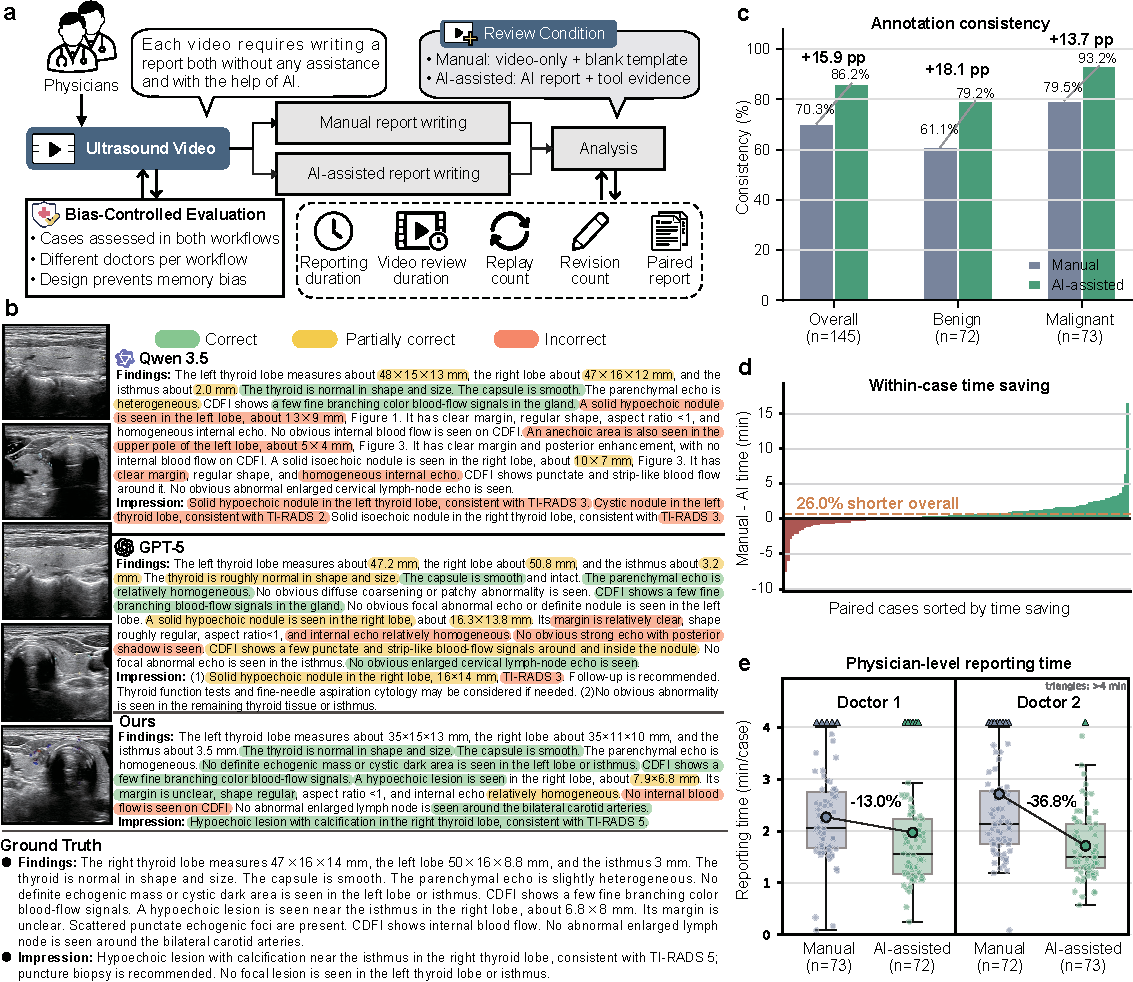
\includegraphics[width=\textwidth]{imgs/ReaderStudy2.pdf}
    \caption{Reader study of AI-assisted thyroid ultrasound reporting. \textbf{a}, Cross-over reader-study design. Each ultrasound video was interpreted under both manual and AI-assisted conditions by different physicians, reducing recall bias while enabling paired case-level comparisons. \textbf{b}, Representative malignant thyroid nodule case comparing reports generated by Qwen 3.5, GPT-5 and ThyroidXAgent with the reference report. Text spans are annotated as correct, partially correct or incorrect according to medical-semantic concordance; ThyroidXAgent shows closer agreement with the reference in this example. \textbf{c}, Annotation consistency of manual and AI-assisted reports, shown overall and stratified by benign and malignant cases. \textbf{d}, Case-level reporting-time reduction, defined as manual minus AI-assisted reporting time and ranked across paired cases. \textbf{e}, Physician-level reporting time under the manual and AI-assisted conditions.}
    \label{fig:reader_study}
\end{figure}



\section{Discussion}

This study reframes thyroid ultrasound AI as an auditable case-level evidence workflow rather than a collection of isolated prediction tasks. The principal contribution of ThyroidXAgent is not a new standalone segmentation, classification or report-generation model, but a shared evidence architecture in which lesion masks, measurements, probabilities, radiomic descriptors, uncertainty signals and report clauses remain visible, editable and reusable across the diagnostic process. Across heterogeneous datasets, this formulation improved nodule segmentation and benign-malignant classification, supported adaptation to additional malignant-lesion tasks, enhanced evidence-grounded reporting and reduced clinician workload. Auditability is therefore embedded in the workflow itself rather than appended retrospectively to a final prediction.

ThyroidXAgent also defines a constrained and clinically practical role for agentic AI. Rather than asking a general-purpose vision-language model to interpret ultrasound images directly, the agent plans case-specific analyses, routes inputs to specialized tools, maintains case state and exposes intermediate results for review. Image interpretation and quantitative measurement remain assigned to task-specific models, whereas the agent provides coordination and evidence management across them. This division of labour extends emerging medical-agent frameworks centred on planning, tool use and coordinated clinical workflows~\cite{Qiu2024NatMachIntellAgenticSystems,Zou2025LancetAgenticTeammates,Moritz2025NatBMECoordinatedAgents}. Its value lies less in unrestricted autonomy than in making heterogeneous model outputs coherent, traceable and correctable.

The shared evidence record further distinguishes ThyroidXAgent from a conventional fixed pipeline. A corrected lesion mask can be propagated to measurement, radiomics, classification and reporting, while anatomical context, malignancy estimates and lesion descriptors can be reused when constructing the diagnostic impression. The same evidence-producing tools could consequently be redirected towards lymph-node metastasis prediction and thyroid carcinoma subtype classification without rebuilding the complete workflow. Report generation provides a particularly stringent demonstration of this design: rather than producing unconstrained free text, ThyroidXAgent assembles report statements from structured clinical evidence. ThyClinScore complements this approach by evaluating lesion matching, clinically relevant attributes and report completeness, thereby capturing errors in location, size or morphology that may be missed by conventional lexical-overlap metrics.

The reader studies indicate that this evidence-centred formulation can support human-AI cooperation without requiring clinicians to accept an opaque recommendation. AI assistance reduced segmentation and reporting time while preserving meaningful points of clinical control, including lesion-boundary correction, evidence inspection and report editing. These findings should not be interpreted as evidence for replacing clinical judgement. Instead, they suggest that agentic systems can reduce repetitive work while keeping consequential intermediate outputs available for verification and correction. The effectiveness of such systems will ultimately depend not only on predictive accuracy, but also on whether clinicians can identify errors, understand their downstream consequences and efficiently intervene.

Several limitations remain. The evaluations were retrospective, and prospective multicentre studies are needed under real acquisition conditions, changing scanner settings and institution-specific reporting practices. The reader studies included a limited number of physicians and primarily assessed workflow feasibility and efficiency rather than patient-level clinical benefit; in the report-writing study, the AI-assisted cases were read before the manual cases, so the difference between the conditions may include a period effect. ThyroidXAgent also remains dependent on the validity and calibration of its component tools: routing cannot compensate for systematically biased segmentation, incomplete metadata or poorly generalized classifiers, although visible intermediate evidence may make these failures easier to detect~\cite{Wiens2019NatMedDoNoHarm,Obermeyer2019ScienceBias}. More generalizable tool design may further improve cross-domain robustness~\cite{gong2025domain,gong2026intermediate}. ZJH-8K and TN3K were both acquired at Zhujiang Hospital, Southern Medical University; ZJH-8K is therefore treated as a same-centre institutional hold-out test set rather than as an independent external-centre cohort. The public TN3K release lacks patient-linkage metadata needed for a systematic patient-level independence audit against ZJH-8K, and several public cohorts provide only official image-level train/validation/test splits. We mitigated cross-source image overlap by perceptual-hash near-duplicate screening of public training partitions against ZJH-8K and excluded exact matches from reported ZJH metrics (Methods); residual patient-level overlap cannot be excluded where patient identifiers are unavailable. Finally, the template-based reporting strategy may require local adaptation, and learning from clinician corrections will require governance for data quality, privacy, provenance, model versioning and distribution shift. Future work should therefore determine whether evidence-level corrections improve downstream clinical decisions prospectively and whether the shared evidence architecture can support additional imaging tasks without sacrificing reliability or interpretability.


\section{Methods}

\subsection{Datasets and task definitions}
For image segmentation and benign-malignant classification, OpenThyroidDB integrates seven public and institutional ultrasound sources comprising 37{,}713 images (18{,}277 training, 850 validation, 18{,}586 test; Supplementary Table~\ref{tab:dataset_summary}). TN3K~\cite{gong2021multi}, TN5K~\cite{zhang2025tn5000}, ThyroidXL~\cite{duong2025thyroidxl} and PKTN~\cite{sun2025clip} served as internal cohorts for nodule segmentation training; TN3K, TN5K and ThyroidXL additionally provided benign-malignant classification labels. DDTI~\cite{pedraza2015open} and RJH-7K~\cite{shusharina2021segmentation} served as independent external test sets, and ZJH-8K (collected at Zhujiang Hospital, Southern Medical University, which also contributed TN3K) as a same-centre institutional hold-out test set of 6{,}807 images (1{,}068 patients) after excluding ZJH images with exact perceptual-hash matches to TN3K training data, with acquisitions between 2016 and 2023: DDTI and ZJH-8K for both tasks, RJH-7K for segmentation only. The full ZJH-8K pool comprised 7,958 images from 1,149 patients before this exclusion. To construct the expert pool, we merged training portions across datasets into stacked training sets, with the largest containing 18,277 images. The included cohorts differed markedly in sample size, class balance and lesion characteristics (Supplementary Fig.~\ref{fig:SegCls_statistics}). For the public cohorts, reference segmentation masks, benign-malignant labels and train/validation/test splits followed the original releases. Cohorts without patient identifiers used the official image-level splits; where patient identifiers were available (ThyroidXL and ZJH-8K), all images of a patient were kept in the same split. Masks and labels were not imputed: images without a valid reference mask or label were excluded from the corresponding task, so that classification on DDTI used its 349 labelled images. Before inference, uniform black margins at the image borders were detected by intensity thresholding and cropped with the same rule for all cohorts. Benign-malignant labels for ZJH-8K were based on postoperative histopathology, supplemented by fine-needle aspiration cytology where applicable, and referred to the target nodule in each image. Reference segmentation masks outlining the target nodule were delineated by ultrasound or radiology physicians of the hospital, and disagreements were resolved by senior review.

For malignant-lesion stratification, two additional tasks were evaluated on the malignant primary-lesion images of ZJH-8K: central lymph-node metastasis (LNM) prediction and classification of classic versus follicular-variant papillary thyroid carcinoma (PTC). The LNM label was the case-level postoperative pathological status of the central compartment (CN0, absent; CN1, present). The subtype label was classic versus follicular-variant PTC on postoperative histology of the index lesion; oncocytic and clear-cell variants, each found in fewer than ten patients, were excluded. Only primary-lesion images were used as inputs; dedicated lymph-node ultrasound images were not used. Among 647 malignant patients, 4,028 primary-lesion images had both central LNM and PTC-subtype labels (after the perceptual-hash exclusion described above) and were split by patient into a development set (3,227 images, 517 patients) and a hold-out test set (801 images, 130 patients; random 20\% of patients, seed 42) shared by both tasks, so that no patient appeared in both sets. At the patient level, LNM was CN0/CN1 in 377/140 (development) and 95/35 (hold-out); PTC subtype was classic/follicular-variant in 466/51 and 117/13. Five additional malignant images lacked both labels and were excluded from these tasks. Models were evaluated with patient-stratified five-fold cross-validation on the development set, then trained once on the full development set and evaluated on the hold-out set. The task-specific DINOv3 classifiers were not initialized from the benign-malignant experts and used the same training augmentation as the other classification experts (synchronized random horizontal and vertical flips). For each patient, image-level probabilities were averaged to give a patient-level score, and AUROC and AUPRC were computed at the patient level, with 95\% confidence intervals from 1,000 patient-level bootstrap resamples.

NHC-MISD-TUS external evaluation used a private, multicentre, test-only thyroid ultrasound subset authorized from the National Health Commission Medical Imaging Standard Database (NHCMISD); it was not used to train the stacked OpenThyroidDB segmentation or classification experts. The release provides 35 anonymized contributing site identifiers and image-level external-test counts of 8{,}721 gland-segmentation test images, with 6{,}384 nodule-segmentation and 4{,}999 benign--malignant classification images where labels were available (per-centre evaluable counts in Supplementary Tables~\ref{tab:gland_dice}--\ref{tab:binary_auprc}; between-centre heterogeneity in Supplementary Table~\ref{tab:nhc_heterogeneity}). Hospital names, patient-level totals, nodule-level totals and scanner inventories were not disclosed under the governing de-identification and data-use conditions; participating units contribute de-identified cases through a standardized intake and quality-control workflow on the database platform.

\subsection{Agent workflow controller and evidence store}
ThyroidXAgent decomposes each case into tool calls and structured intermediate outputs. The workflow contains an expert pool for image segmentation and classification, a radiomics branch, a tabular prediction branch, post hoc explanation modules, anatomical-context parsers, measurement tools and report-generation modules. The LLM router operates on structured summaries rather than raw ultrasound images. During inference, it receives candidate masks, class probabilities, confidence estimates, radiomic descriptors and metadata such as image resolution, device and data source. It emits a strict JSON decision that records the selected output, supporting evidence and uncertainty signals. These outputs are normalized into a case-level evidence store containing masks, measurements, class probabilities, radiomic descriptors, explanation objects, warnings and report clauses. The evidence store is used for final prediction, report assembly and clinician review, and clinician corrections can be written back to the same record for subsequent use.

\subsection{Segmentation, classification and radiomics}
ThyroidXAgent coordinates a heterogeneous expert pool, an LLM router and a radiomics branch for image segmentation and classification: the expert pool generates candidate masks and class probabilities, the router selects the most reliable candidate based on quality metrics and case-level metadata, and the radiomics branch provides an independent classification signal. For image segmentation and classification, the expert pool is designed as a heterogeneous ensemble rather than a single model to reduce sensitivity to dataset bias~\cite{torralba2011unbiased,liu2024decade} (Supplementary Fig.~\ref{fig:ThyroidXAgent_for_seg_and_cls}). Each expert typically uses a DINOv3-based backbone~\cite{simeoni2025dinov3} with a task-specific lightweight head, though task-specific external models can also be assembled for specialized classification targets. To encourage complementary generalization profiles, these experts were trained under varying configurations along three dimensions: stacked-training composition, input resolution (128, 224 and 448 pixels), and whether DINOv3 pretrained weights were loaded or the backbone was trained from scratch. For the segmentation branch, backbone dilation rates were additionally varied to produce experts with different receptive-field profiles. This heterogeneity exposes individual experts to progressively broader data distributions, so that the router can select the most reliable candidate for each case rather than relying on a single model's bias. The effect of these stacked-training configurations on cross-dataset performance is reported in Supplementary Table~\ref{tab:stacked_performance}.

Within this pool, the segmentation branch uses a U-Net-style decoder with skip fusion to preserve fine boundary detail, and is optimized with a combined loss that balances pixel-level supervision with region-level overlap:
\[
\mathcal{L}_{\text{seg}} = \mathcal{L}_{\text{wBCE}}(m, \hat{m}) + \mathcal{L}_{\text{IoU}}(m, \hat{m}),
\]
where $m$ denotes the ground-truth mask, $\hat{m}$ the prediction, $\mathcal{L}_{\text{wBCE}}$ the class-weighted binary cross-entropy and $\mathcal{L}_{\text{IoU}}$ the intersection-over-union loss. The classification branch pools backbone features using global average and max pooling, followed by a compact attention head. To mitigate class imbalance, generalized logit adjustment (GLA)~\cite{menon2020long} is applied to the classification logits:
\[
\tilde{z}_c = z_c + \tau\log(\pi_c),
\]
where $z_c$ is the logit for class $c$, $\pi_c$ is the empirical class prior estimated from the training set, and $\tau$ is adaptively set based on the class imbalance ratio. Binary classification tasks use BCE on the adjusted logits, whereas multi-class tasks use cross-entropy on the adjusted logits. Each expert produces a class probability $p_i$; the per-expert confidence $c_i$ is taken as the maximum softmax output of the classification head for expert $i$.

Once these per-expert outputs are available, task-specific quality metrics are computed across them to inform the selection: morphological plausibility such as area, circularity and compactness, and inter-model agreement measured by pairwise IoU and HD95, for segmentation; and prediction uncertainty such as entropy and margin, and class consensus, for classification. The LLM router then selects the best mask and classification result by reasoning over these quality metrics, per-expert confidence estimates and case-level metadata, rather than by simple confidence maximization or majority voting. Depending on the configured ensemble size, the router selects either the single best expert or a subset of experts for weighted ensemble fusion. This routing design allows the system to adapt its selection to the acquisition conditions of each case, rather than relying on a fixed model ranking.

To provide a classification signal independent of the image-based experts, the radiomics branch processes the selected mask. The mask is first refined via connected-component analysis to remove isolated noisy regions when multiple disconnected components are present. Two-dimensional PyRadiomics descriptors~\cite{van2017computational}, including shape, intensity and texture features, are then extracted from the refined mask-image pair, yielding the radiomic descriptor vector. These descriptors are passed to AutoGluon-tabular classifiers~\cite{erickson2020autogluon}, which ensemble multiple tabular models under automated hyperparameter optimization. The resulting tabular class prediction is stored alongside the router's selection in the case-level evidence store, providing a complementary interpretive signal for clinician review. After selection, SHAP analysis~\cite{lundberg2017unified} is applied to the tabular classifier to estimate global and local feature contributions, while Grad-CAM~\cite{selvaraju2017gradcam} is applied to the selected segmentation model to visualize the image regions driving its mask prediction. These post hoc explanations are stored in the evidence store for clinician inspection. Importantly, the same segmentation, radiomics, tabular classification and explanation workflow is reused across benign-malignant classification and additional malignant-lesion stratification tasks, including central LNM prediction and PTC subtype classification; only task-specific classifier fine-tuning, the task description supplied to the router, and, where applicable, external model assembly are changed. This reuse allows the agent workflow to be redirected to new clinical questions without rebuilding the diagnostic pipeline.

\subsection{ThyClinScore}
ThyClinScore evaluates thyroid ultrasound reports as a structured clinical semantic agreement task. It measures both report completeness and semantic consistency with the reference report. Semantic consistency is assessed at two levels: gland-level agreement for thyroid measurements, parenchymal morphology and gland-level vascularity; and lesion-level agreement for lesion detection, lesion size, lesion descriptors and lesion-level vascularity. Size and vascularity can therefore be scored at either level when the corresponding fields are available, whereas morphology mainly captures concept-level agreement in gland and parenchymal descriptions.

For each case, the reference report \(R^{\mathrm{gt}}\) and generated report \(R^{\mathrm{pred}}\) were converted into a shared schema containing thyroid measurements, parenchymal findings, lesion attributes, lymph-node findings and diagnostic impressions. Measurements were standardized in millimetres, categorical fields were restricted to predefined thyroid ultrasound descriptors, and absent information was represented as null. The schema retained clinically relevant information, including lesion location, size, composition, echogenicity, margin, shape, echogenic foci, vascularity and TI-RADS category. These fields supported subsequent lesion-level matching and semantic scoring.

At the lesion level, reference and predicted lesions were first matched before lesion detection and attribute agreement were evaluated. Let \(G=\{g_i\}_{i=1}^{m}\) denote reference lesions and \(P=\{p_j\}_{j=1}^{n}\) denote predicted lesions. For each candidate pair, we computed
\[
S_{ij}=M^{\mathrm{loc}}_{ij}
\left(\alpha_sS^{\mathrm{size}}_{ij}+\beta_fS^{\mathrm{feat}}_{ij}\right),
\qquad
S^{\mathrm{size}}_{ij}=\frac{\min(d_i,d_j)}{\max(d_i,d_j)},
\]
where \(d_i\) and \(d_j\) are maximum lesion diameters, \(M^{\mathrm{loc}}_{ij}\in\{0,1\}\) is a hard anatomical-location gate, and \(S^{\mathrm{feat}}_{ij}\in\{0,0.5,1\}\) scores lesion-composition agreement. Explicit left-right mismatches were assigned \(M^{\mathrm{loc}}_{ij}=0\). We solved the bipartite assignment using \(c_{ij}=1-S_{ij}\) and retained pairs above a predefined threshold. Matched pairs were treated as true positives, unmatched reference lesions as false negatives and unmatched predicted lesions as false positives, from which lesion-level precision, recall, F1 and false discovery rate were calculated.

Numerical measurements were scored using mean relative error (MRE), applied to thyroid lobe and isthmus measurements at the gland level and lesion dimensions at the lesion level. For paired dimensions \(K\),
\[
\mathrm{MRE}_{K}=\frac{1}{|K|}\sum_{k\in K}
\frac{|p_k-g_k|}{\max(|g_k|,\epsilon)},\qquad
s_{\mathrm{size}}(\mathrm{MRE}_{K};\tau)=2^{-(\mathrm{MRE}_{K}/\tau)^2},
\]
where \(\epsilon\) provides numerical stability and \(\tau\) controls tolerance to size error. Vascularity was evaluated at either level when available. It was discretized into four grades, from absent flow to markedly increased flow, and scored as
\[
s_{\mathrm{vasc}}=\max\left(0,1-\frac{|v^{\mathrm{gt}}-v^{\mathrm{pred}}|}{3}\right).
\]
Morphological consistency was computed at the concept level for gland and parenchymal descriptions. A thyroid-specific lexicon mapped report phrases to concepts covering echogenicity, texture, margin, shape, calcification, posterior acoustic features and composition. For concept sets \(C^{\mathrm{gt}}\) and \(C^{\mathrm{pred}}\), morphology agreement was scored by concept F1. For matched lesions, categorical descriptors were scored by mean accuracy over reference-present fields, including composition, echogenicity, margin, shape and echogenic foci.

Gland-level and lesion-level assessments were combined into a clinical consistency score \(C\), which aggregates thyroid-size agreement, lesion-size agreement, vascularity agreement, lesion-detection F1, lesion-feature accuracy and morphology agreement. Components not applicable to either report were excluded from the denominator, whereas reference-present fields missing from the generated report contributed zero:
\[
C=\frac{\sum_{q\in\mathcal{Q}}w_qs_q}{\sum_{q\in\mathcal{Q}}w_q},
\]
where \(s_q\) denotes a valid component score and \(w_q\) its predefined weight. Report completeness \(B\) was defined as the weighted fraction of required information present in the generated structured report:
\[
B=\frac{\sum_{r\in\mathcal{R}}u_rb_r}{\sum_{r\in\mathcal{R}}u_r}.
\]
The completeness groups were thyroid measurements, parenchyma, lesions, impression and lymph-node description; \(b_r\) indicates presence of group \(r\), and \(u_r\) denotes its predefined weight. The final ThyClinScore was
\[
\mathrm{ThyClinScore}=
\left[\lambda B+(1-\lambda)C\right]
\left[\eta+(1-\eta)F_L\right],
\]
for cases with reference lesions, where \(\lambda\) balances completeness and clinical consistency, and \(\eta\) controls the minimum lesion-detection gate. For reports without reference lesions, the gate was omitted. This design rewards complete and semantically consistent reports while penalizing missed or hallucinated lesions.

The default parameters of ThyClinScore (\(\lambda=0.3\), \(\eta=0.5\), a lesion-matching threshold of 0.5, \(\alpha_s=0.7\), size tolerances \(\tau\) of 0.2 and 0.3 for gland and lesion measurements, consistency weights \(w_q\) of 0.2, 0.15, 0.15, 0.15, 0.2 and 0.15 for thyroid size, lesion size, vascularity, lesion detection, lesion features and morphology, and completeness weights \(u_r\) of 0.25, 0.25, 0.35, 0.1 and 0.05 for thyroid measurements, parenchyma, lesions, impression and lymph nodes) were set heuristically and were not optimized on any dataset. We assessed their influence by recomputing ThyClinScore for all models under 120 configurations, in which each parameter was varied singly and in three joint grids (\(\lambda\) from 0.1 to 0.5, \(\eta\) and the matching threshold from 0.3 to 0.7, \(\alpha_s\) from 0.5 to 0.9, \(\tau\) by \(\pm\)50\% and each weight from 0.5 to 1.5 times its default), and compared the ranking of the models.

For clinician validation, two clinicians independently rated 270 reports of 90 cases (30 cases per test set, stratified by the number of reference lesions; the ThyroidXAgent report and two baseline reports per case) against the reference report on clinical accuracy, factual consistency, completeness, readability and clinical usability on a scale of 1 to 5, blinded to the system; a report's rating was the mean of the available ratings. Correlations with the ratings were estimated with Spearman's \(\rho\) and case-bootstrap 95\% CIs (10,000 resamples), and inter-rater agreement with ICC(2,1). In addition, we selected \(\lambda\) and \(\eta\) on the SMU-HMC ratings among the 25 combinations of the sensitivity analysis. The best combination (\(\lambda=0.4\), \(\eta=0.7\)) correlated only slightly more strongly with the clinical-accuracy rating than the default values (0.459 versus 0.437; Supplementary Table~\ref{tab:thyclinscore_clinician}) and, with these values fixed, ThyroidXAgent still had the highest mean ThyClinScore on all three test sets. We therefore report results with the default parameters, which had been set before any clinician ratings were collected.



\subsection{Report generation}
For the reporting branch, thyroid ultrasound reporting was formulated as a case-level evidence-to-report task rather than as single-image captioning. Given an image set \(\mathcal{I}=\{I_j\}_{j=1}^{N}\), which could include video frames, static images, multiple anatomical views, greyscale ultrasound and colour Doppler images, the workflow generated a structured report \(R\) and an accompanying evidence trace. The report covered thyroid gland morphology, nodule-level findings, lymph-node findings when present and the diagnostic impression. The trace recorded the intermediate observations supporting each report component.

Input preparation converted heterogeneous case files into image priors for subsequent planning (Supplementary Fig.~\ref{fig:report_generation_multimodal_interface}). Images were standardized and processed by auxiliary modules for region-of-interest cropping, anatomical-context parsing, colour Doppler identification, nodule-presence triage and pixel-spacing estimation when required. The resulting priors encoded region, view, modality, Doppler status and nodule likelihood. They were used to guide downstream analysis, rather than inserted directly into report text.

The reporting workflow was packaged as a single reusable skill. The skill defined the reporting objective, evidence schema, staged diagnostic process and constraints for evidence-grounded writing. External agents invoked this skill through a Workflow Model Context Protocol (MCP) server, which exposed high-level case operations for input preparation, case initiation, plan review and approval, and report and evidence retrieval. Low-level operations, including segmentation, classification, measurement and captioning, remained internal to the workflow. This separated a stable public interface from the image-processing and model-execution details needed to construct reliable evidence. It also made the resulting report traceable for clinician review.

After input preparation, ThyroidXAgent used a planner-executor design~\cite{wang_plan-and-solve_2023}. The planner received the skill instructions, tool contract and image priors, and generated a case-specific staged task graph covering gland assessment, nodule analysis, lymph-node assessment, evidence fusion and report generation. This graph provided global diagnostic constraints, while allowing case-specific execution. In the deployable workflow, the plan could be inspected and approved before model execution. The executor then followed the approved graph and used ReAct-style local decision-making~\cite{yao_react:_2022} to select images and internal tools according to intermediate observations. For example, cases without nodule priors could bypass nodule-feature classification, whereas lateral-neck images could trigger lymph-node screening before report assembly.

Selected model operations were executed by the internal diagnostic runtime. In deployment, the Workflow MCP process remained lightweight and delegated GPU inference to a separate tool service. The runtime could call preprocessing modules, gland captioning, spacing prediction, thyroid and nodule measurement, nodule segmentation, nodule-feature classification, malignancy classification, cervical lymph-node screening and nodule-level fusion. Their outputs were normalized into a shared evidence object before language generation. Gland-level evidence included thyroid lobe and isthmus measurements, parenchymal morphology and vascularity. Nodule-level evidence included anatomical location, size, composition, echogenicity, margin, shape, echogenic foci, vascularity, segmentation-derived measurements and risk-related predictions. Lymph-node evidence summarized cervical-region screening results. When multiple views described the same lesion, the fusion stage consolidated compatible findings into case-level nodule entries and retained warnings for incomplete or conflicting outputs.

Report text was generated by controlled data-to-text assembly~\cite{rebuff_data2text_2020}. To reduce factual hallucination risk~\cite{farquhar2024detecting}, ThyroidXAgent used training-free BM25 template retrieval, slot filling and clause assembly rather than unconstrained free-text decoding. Corresponding template libraries were constructed from the SMU-HMC and KMVE datasets. The SMU-HMC was derived from 7,147 quality-controlled reports after excluding all reports from the 400 patients reserved for internal testing. The KMVE library was constructed from the 1,313 reports of its training partition that remained after excluding 406 reports that were near-duplicates of test reports. During template construction, whole reports were decomposed into five clinically defined clause categories: thyroid measurement, gland morphology, nodule findings, lymph-node findings and ultrasound impression. Case-specific content was replaced by slot placeholders, identical templates were merged, infrequent templates were removed by fixed frequency thresholds, and manual review removed 57 gland and measurement templates that are not typical of complete routine reports, such as those from postoperative, emergency or bedside examinations. During inference, the evidence object assembled through tool execution was partitioned into corresponding evidence blocks and converted into category-specific BM25 queries. Retrieved templates served as linguistic frames; slot filling inserted case-specific measurements, descriptors, TI-RADS-relevant information, risk categories and other tool-derived evidence, and clause assembly combined the completed findings and impression clauses into the final report.

Notably, KMVE contains only the ultrasound findings section and does not provide original measurement values. The KMVE library was therefore built with the same procedure but kept the structure and linguistic style of the KMVE findings: nodule sizes were masked as in the KMVE reports, gland sentences were selected according to the gland size, parenchymal echo and parenchymal vascularity reported by the gland-captioning tool, and the library was used in accordance with the original findings-only evaluation protocol. Because tool execution was decoupled from report realization, the retrieval libraries could be exchanged in a plug-and-play manner to align generated reports with centre- or corpus-specific writing conventions, without retraining the upstream image-analysis tools or modifying the underlying evidence schema. The same procedure can be used to construct updated retrieval libraries from new report sources (Supplementary Fig.~\ref{fig:report_generation_template_bank}). To assess centre-specific template effects, we exchanged the clause templates between the SMU-HMC and KMVE libraries while keeping the tool outputs and the report format of each test set. The lexical metrics decreased substantially (ROUGE-L by 0.10 to 0.29 and BLEU-4 by 0.14 to 0.28), whereas ThyClinScore decreased much less (by 0.05 in SMU-HMC and KMVE and by 0.01 in ZJH-TS; Supplementary Table~\ref{tab:template_exchange}), indicating that exchanging the templates mainly changed how the findings were worded and organized, while most of the clinically relevant content was retained.

For comparison, five general-purpose multimodal models (GPT-4o~\cite{openai_gpt4_2024}, GPT-5~\cite{openai2025gpt5systemcard}, Gemini 2.5 Pro~\cite{comanici_gemini_2025}, Qwen3.5 Plus~\cite{yang_qwen3_2025} and Claude Sonnet 4.6, accessed through an API) and MedGemma~\cite{sellergren2025medgemma} received a prompt specifying the report structure with three example reports in the reporting format of the dataset (few-shot prompting), together with up to five images sampled at random from each case in SMU-HMC and ZJH-TS (seed 42) or the two images of each case in KMVE. LLaVA-Med~\cite{li_llavamed_2023} received two images and an English version of the prompt, and its output was translated into Chinese with GPT-4o-mini. The KMVE model~\cite{li_ultrasound_2024}, which was trained on the KMVE dataset, was applied to two images per case on SMU-HMC and ZJH-TS.

The final artefact consisted of the report text and its supporting evidence trace. Clinicians or external agents could inspect the diagnostic plan, verify the evidence used for each statement, review warnings and edit the generated report. Corrected reports could then be returned to the case-level evidence store for subsequent review and model updating. This design kept report generation constrained by structured clinical evidence while preserving a reviewable path from image inputs to final report statements.


\subsection{Reader studies and statistical analysis}
For segmentation review, clinicians corrected AI-generated masks, and correction time and paired Dice scores were compared with manual segmentation. For report writing, two physicians evaluated 145 thyroid ultrasound videos with annotation-derived case labels in a cross-over design. Each case was interpreted under both manual and AI-assisted conditions, but by different physicians, to reduce memory and recall bias. The allocation of each case to the two conditions and the reading order were randomized, and each physician read the AI-assisted cases in one block and the manual cases in a second block 8 to 12 days later. In the manual condition, physicians reviewed the ultrasound video and completed a blank structured-report template. In the AI-assisted condition, they reviewed an AI-generated draft together with the supporting tool-derived evidence and revised the report as required. We recorded reporting time, video-review time and the final submitted report for each assessment. Reporting efficiency was assessed at both the case and physician levels, with case-level time saving defined as the manual minus AI-assisted reporting time.

For the analysis of annotation consistency, frame-level benign and malignant bounding-box annotations were aggregated into case-level labels. Cases containing any malignant annotation were classified as malignant or suspicious, whereas cases containing only benign annotations were classified as benign. This yielded 145 labelled cases, comprising 72 benign and 73 malignant or suspicious cases. A prespecified rule-based procedure assigned each submitted report to a benign or low-risk, malignant or suspicious, or ambiguous direction using TI-RADS categories and diagnostic terms. Annotation consistency was defined as agreement between the diagnostic direction of the report and the annotation-derived case label, with ambiguous reports counted as disagreements, and was summarized overall and within the benign and malignant or suspicious strata. The difference between conditions was estimated over the 145 cases paired by case, with a case-bootstrap 95\% CI (10,000 resamples) and an exact McNemar test, and in a linear probability model with the condition and the physician as covariates. For statistical analysis, performance was summarized using the primary metric for each task: Dice and HD95 for segmentation, AUROC and AUPRC for classification, conventional natural-language generation metrics for report wording, and ThyClinScore and its submetrics for report semantics. Confidence intervals in the supplementary tables were estimated by nonparametric bootstrap resampling of the test set; for image segmentation and classification, resampling was clustered by patient where patient identifiers were available, with 1{,}000 resamples. Cross-cohort means were unweighted averages of the cohort-level estimates. Correlations between report metrics and the location-aware LLM judge were evaluated using two-sided Pearson correlation tests.
The reports compared with the baselines were drafts generated directly by ThyroidXAgent without physician review. We consider that an AI-generated report must be reviewed and finalized by a physician, and we therefore developed safety rules that facilitate this review (Supplementary Table~\ref{tab:safety_rules} and Supplementary Fig.~\ref{fig:report_generation_planning_execution_review}c). The rules have two layers: the first withholds statements that the tool evidence does not support and states them as not assessed, and the second marks each sentence of the draft for the reviewing physician as red for mandatory review, yellow for a focused check, grey for items to be completed by the physician or green when no safety rule is triggered. We evaluated the rules in an additional study in which two physicians each reviewed and completed the drafts of 35 videos drawn at random from the 145, and recorded the number of nodules and the benign or malignant tendency of each nodule in each lobe and the isthmus, which served as the reference for the errors of the drafts.


\section{Data availability}
%The public datasets used in this study are available from their original sources, as cited in the Methods and Supplementary Table~\ref{tab:dataset_summary}. Institutional ultrasound images and reports contain clinical data and are not publicly released in raw form because of privacy and institutional governance restrictions. De-identified derived data, dataset splits and evaluation outputs can be made available from the corresponding authors upon reasonable request and subject to institutional approval. 
%The NHCMISD dataset was collected from real world clinical ultrasound cases provided by the National Health Commission Medical Imaging Standard Database, for which the  co-author, Prof. Dexing Kong, has authorized access. All data usage complied with relevant institutional and regulatory requirements.
The public datasets used in this study are available from their original sources, as cited in the Methods and Supplementary Table~\ref{tab:dataset_summary}. The publicly released data associated with this study are available through ThyroidOpenDB at \url{https://huggingface.co/datasets/MedXAgent/ThyroidOpenDB}.
The study was approved by the Medical Ethics Committee of Zhujiang Hospital, Southern Medical University (approval no. 2026-KY-081-01).

Institutional ultrasound images and reports, and the NHC-MISD-TUS subset from the National Health Commission Medical Imaging Standard Database, are not publicly released because of privacy and data-governance restrictions. NHC-MISD-TUS access is governed by a cooperation and data-compliance agreement with the database programme. De-identified derived data, dataset splits and evaluation outputs not included in ThyroidOpenDB may be available from the corresponding authors upon reasonable request and subject to institutional approval.


\section{Code availability}
%The source code, trained model checkpoints and report-generation templates will be released after institutional review. Until public release, code required to reproduce the reported analyses is available from the corresponding authors upon reasonable request.
The source code for ThyroidXAgent is publicly available on GitHub at \url{https://github.com/MedXAgent/ThyroidXAgent}. The website will be made available after acceptance. The trained model weights are available on Hugging Face at \url{https://huggingface.co/MedXAgent/ThyroidXAgent}. The repositories contain the resources required to reproduce the reported computational analyses.

\section{Acknowledgements}
This work was supported in part by the National Natural Science Foundation of China (Grant No. 62322608), the Zhejiang Provincial Natural Science Foundation of China (Grant No. LQN26F020029), and the Natural Science Foundation of Guangdong Province (Grant No. 2024A1515010255).


\section{Author contributions}

\begin{itemize}
    \item \textbf{Conceptualization:} H.G. and G.L.
    \item \textbf{System development:} S.C., B.W. and X.X.
    \item \textbf{Computational evaluation:} S.C., B.W. and S.W.
    \item \textbf{Visualization:} S.C., B.W. and H.G.

    \item \textbf{Reader study:} H.W., Q.L. and F.C.
    \item \textbf{Data curation and organization:} H.G., S.C., B.W., Y.W., G.Y., H.W., M.M., D.K., Q.L., W.L. and F.C.
    \item \textbf{Writing--original draft:} H.G., Y.W., S.C. and B.W.
    \item \textbf{Writing--review and editing:} All authors.
    \item \textbf{Supervision:} Q.L., W.L., F.C. and G.L.
\end{itemize}

\section{Competing interests}
The authors have no conflicts of interest.

\clearpage
\begin{appendices}

\renewcommand{\thefigure}{S\arabic{figure}}
\renewcommand{\thetable}{S\arabic{table}}
\setcounter{figure}{0}
\setcounter{table}{0}

\section*{Supplementary information}
\phantomsection
\addcontentsline{toc}{section}{Supplementary information}

\newcommand{\suppcontentsline}[3]{%
  \noindent\hyperref[#1]{\textbf{#2}}\enspace #3\dotfill\pageref{#1}\par
}

\subsubsection*{Supplementary figures}
% Requires \usepackage{hyperref} in the main document preamble.

% Framework and data structure
\suppcontentsline{fig:ThyroidXAgent_for_seg_and_cls}{\hyperref[fig:ThyroidXAgent_for_seg_and_cls]{Figure S1.}}{\hyperref[fig:ThyroidXAgent_for_seg_and_cls]{ThyroidXAgent architecture for thyroid nodule segmentation and classification}}
\suppcontentsline{fig:SegCls_statistics}{\hyperref[fig:SegCls_statistics]{Figure S2.}}{\hyperref[fig:SegCls_statistics]{Dataset composition and lesion distributions across thyroid ultrasound cohorts}}

% Segmentation and classification
\suppcontentsline{fig:BM_cases}{\hyperref[fig:BM_cases]{Figure S3.}}{\hyperref[fig:BM_cases]{Case-level explanations for thyroid nodule classification}}

% Report generation
\suppcontentsline{fig:report_generation_multimodal_interface}{\hyperref[fig:report_generation_multimodal_interface]{Figure S4.}}{\hyperref[fig:report_generation_multimodal_interface]{Multimodal input processing and case interaction in ThyroidXAgent}}
\suppcontentsline{fig:report_generation_planning_execution_review}{\hyperref[fig:report_generation_planning_execution_review]{Figure S5.}}{\hyperref[fig:report_generation_planning_execution_review]{Planning, tool execution and clinician review in the report-generation workflow}}
\suppcontentsline{fig:report_generation_template_bank}{\hyperref[fig:report_generation_template_bank]{Figure S6.}}{\hyperref[fig:report_generation_template_bank]{Template-bank construction for centre-specific report generation}}
\suppcontentsline{fig:RG_CaseReview}{\hyperref[fig:RG_CaseReview]{Figure S7.}}{\hyperref[fig:RG_CaseReview]{Qualitative comparison of thyroid ultrasound report generation}}

\subsubsection*{Supplementary tables}

% Framework and data structure
\suppcontentsline{tab:dataset_summary}{\hyperref[tab:dataset_summary]{Table S1.}}{\hyperref[tab:dataset_summary]{Composition and data splits of the multicentre thyroid ultrasound benchmark}}
\suppcontentsline{tab:dataset_comparison}{\hyperref[tab:dataset_comparison]{Table S2.}}{\hyperref[tab:dataset_comparison]{Characteristics of public and institutional thyroid ultrasound datasets}}

% Segmentation and classification
\suppcontentsline{tab:seg_performance}{\hyperref[tab:seg_performance]{Table S3.}}{\hyperref[tab:seg_performance]{Cross-dataset generalization for thyroid nodule segmentation}}
\suppcontentsline{tab:cls_performance}{\hyperref[tab:cls_performance]{Table S4.}}{\hyperref[tab:cls_performance]{Cross-dataset generalization for benign-malignant thyroid nodule classification}}
\suppcontentsline{tab:Malignant_images_tasks_performance}{\hyperref[tab:Malignant_images_tasks_performance]{Table S5.}}{\hyperref[tab:Malignant_images_tasks_performance]{Performance on malignant thyroid lesion stratification}}
\suppcontentsline{tab:stacked_performance}{\hyperref[tab:stacked_performance]{Table S6.}}{\hyperref[tab:stacked_performance]{Effects of cumulative training-data integration on segmentation and classification}}
\suppcontentsline{tab:gland_dice}{\hyperref[tab:gland_dice]{Table S7.}}{\hyperref[tab:gland_dice]{Centre-specific Dice for thyroid gland segmentation in NHC-MISD-TUS}}
\suppcontentsline{tab:gland_hd95}{\hyperref[tab:gland_hd95]{Table S8.}}{\hyperref[tab:gland_hd95]{Centre-specific HD95 for thyroid gland segmentation in NHC-MISD-TUS}}
\suppcontentsline{tab:nodule_dice}{\hyperref[tab:nodule_dice]{Table S9.}}{\hyperref[tab:nodule_dice]{Centre-specific Dice for thyroid nodule segmentation in NHC-MISD-TUS}}
\suppcontentsline{tab:nodule_hd95}{\hyperref[tab:nodule_hd95]{Table S10.}}{\hyperref[tab:nodule_hd95]{Centre-specific HD95 for thyroid nodule segmentation in NHC-MISD-TUS}}
\suppcontentsline{tab:binary_auroc}{\hyperref[tab:binary_auroc]{Table S11.}}{\hyperref[tab:binary_auroc]{Centre-specific AUROC for benign-malignant classification in NHC-MISD-TUS}}
\suppcontentsline{tab:binary_auprc}{\hyperref[tab:binary_auprc]{Table S12.}}{\hyperref[tab:binary_auprc]{Centre-specific AUPRC for benign-malignant classification in NHC-MISD-TUS}}

% Report generation
\suppcontentsline{tab:auxiliary_tools}{\hyperref[tab:auxiliary_tools]{Table S13.}}{\hyperref[tab:auxiliary_tools]{Performance of preprocessing and executor tools in ThyroidXAgent}}
\suppcontentsline{tab:report_generation_nlg_ci}{\hyperref[tab:report_generation_nlg_ci]{Table S14.}}{\hyperref[tab:report_generation_nlg_ci]{Lexical performance of thyroid ultrasound report generation across datasets}}
\suppcontentsline{tab:report_generation_clinical_ci}{\hyperref[tab:report_generation_clinical_ci]{Table S15.}}{\hyperref[tab:report_generation_clinical_ci]{Clinical semantic performance of thyroid ultrasound report generation across datasets}}
\suppcontentsline{tab:static_rule_controller_radar_metrics}{\hyperref[tab:static_rule_controller_radar_metrics]{Table S16.}}{\hyperref[tab:static_rule_controller_radar_metrics]{Static-pipeline metrics used for report-generation radar plots}}
\suppcontentsline{tab:report_generation_tool_ablation}{\hyperref[tab:report_generation_tool_ablation]{Table S17.}}{\hyperref[tab:report_generation_tool_ablation]{Ablation of tool integration for thyroid ultrasound report generation}}
\suppcontentsline{tab:thyclinscore_clinician}{\hyperref[tab:thyclinscore_clinician]{Table \ref*{tab:thyclinscore_clinician}.}}{\hyperref[tab:thyclinscore_clinician]{Validation of ThyClinScore against clinician ratings}}
\suppcontentsline{tab:template_exchange}{\hyperref[tab:template_exchange]{Table \ref*{tab:template_exchange}.}}{\hyperref[tab:template_exchange]{Effect of exchanging clause templates between report libraries on report-generation performance}}
\suppcontentsline{tab:safety_rules}{\hyperref[tab:safety_rules]{Table \ref*{tab:safety_rules}.}}{\hyperref[tab:safety_rules]{Safety rules for physician review of AI-generated report drafts}}
\suppcontentsline{tab:patient_level}{\hyperref[tab:patient_level]{Table \ref*{tab:patient_level}.}}{\hyperref[tab:patient_level]{Patient-level performance of ThyroidXAgent on ZJH-8K and ThyroidXL}}
\suppcontentsline{tab:nhc_heterogeneity}{\hyperref[tab:nhc_heterogeneity]{Table \ref*{tab:nhc_heterogeneity}.}}{\hyperref[tab:nhc_heterogeneity]{Between-centre heterogeneity in NHC-MISD-TUS}}

% ================================================================
% Supplementary Figures: one figure per page
% ================================================================
\clearpage
% Framework and data structure
\begin{figure}[p]
    \centering
    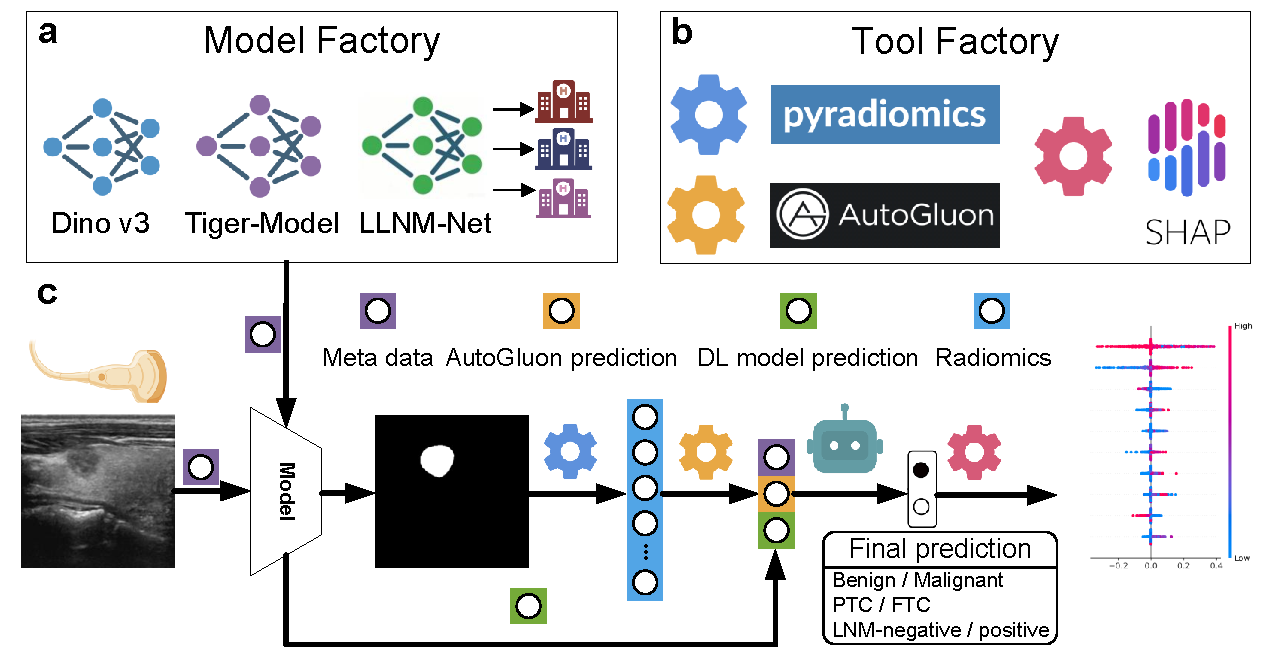
\includegraphics[width=\textwidth,height=0.72\textheight,keepaspectratio]{imgs/ThyroidXAgent_for_seg_and_cls.pdf}
    \caption{ThyroidXAgent architecture for thyroid nodule segmentation and classification. DINOv3-based experts generate candidate segmentation masks and malignancy probabilities. The radiomics branch extracts PyRadiomics features from the selected lesion mask, applies an AutoGluon classifier and computes SHAP attributions. The LLM router integrates the candidate outputs with image metadata, including resolution, device and data source, to select the final prediction and its supporting evidence.}
    \label{fig:ThyroidXAgent_for_seg_and_cls}
\end{figure}
\clearpage

\begin{figure}[p]
    \centering
    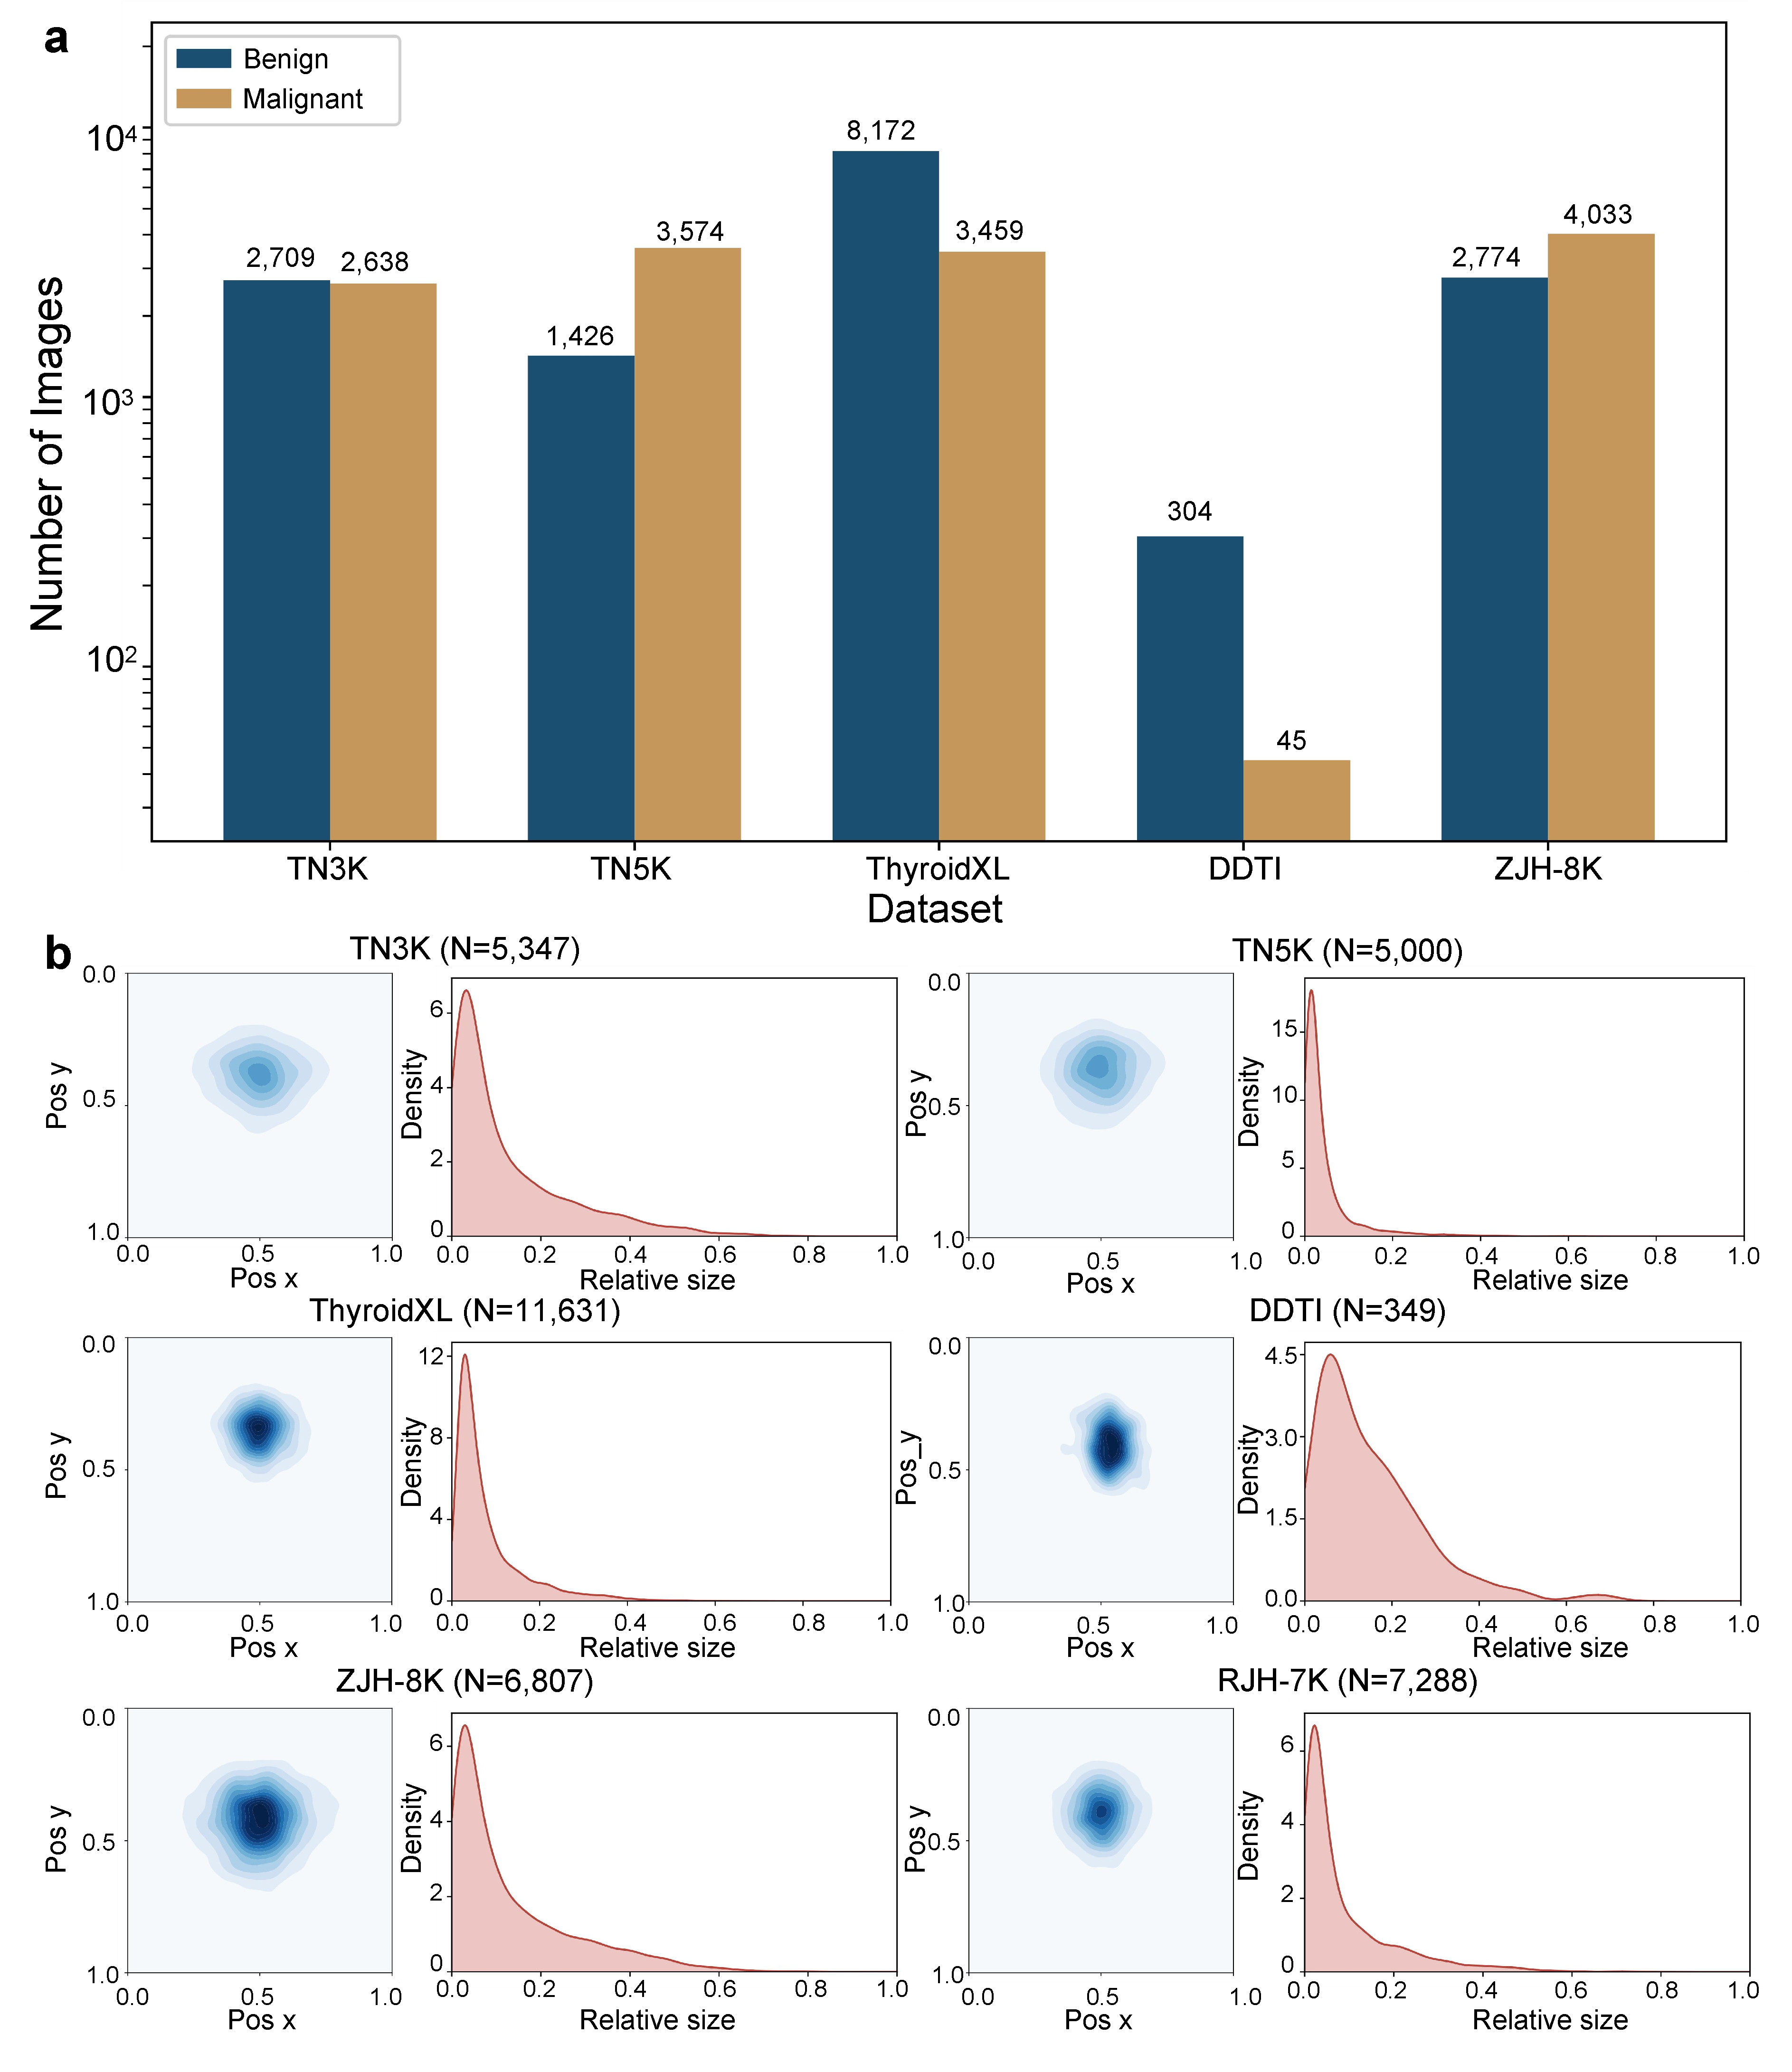
\includegraphics[width=\textwidth,height=0.72\textheight,keepaspectratio]{imgs_sup/SegCls_statistics.pdf}
    \caption{Dataset composition and lesion distributions across thyroid ultrasound cohorts. Top, grouped bar chart comparing the numbers of benign and malignant images in TN3K, TN5K, ThyroidXL, DDTI and ZJH-8K on a logarithmic y axis, highlighting marked variation in cohort size and class balance across cohorts. Bottom, for each of the five datasets, two-dimensional kernel density estimates of normalized lesion-mask centroid positions (left) and relative lesion size distributions, defined as mask area divided by image area (right). All size distributions share a common x-axis range, and all spatial maps use a common density scale, enabling direct cross-dataset comparison of where lesions appear within the ultrasound frame and how large they tend to be.}
    \label{fig:SegCls_statistics}
\end{figure}
\clearpage

% Segmentation and classification
\begin{figure}[p]
    \centering
    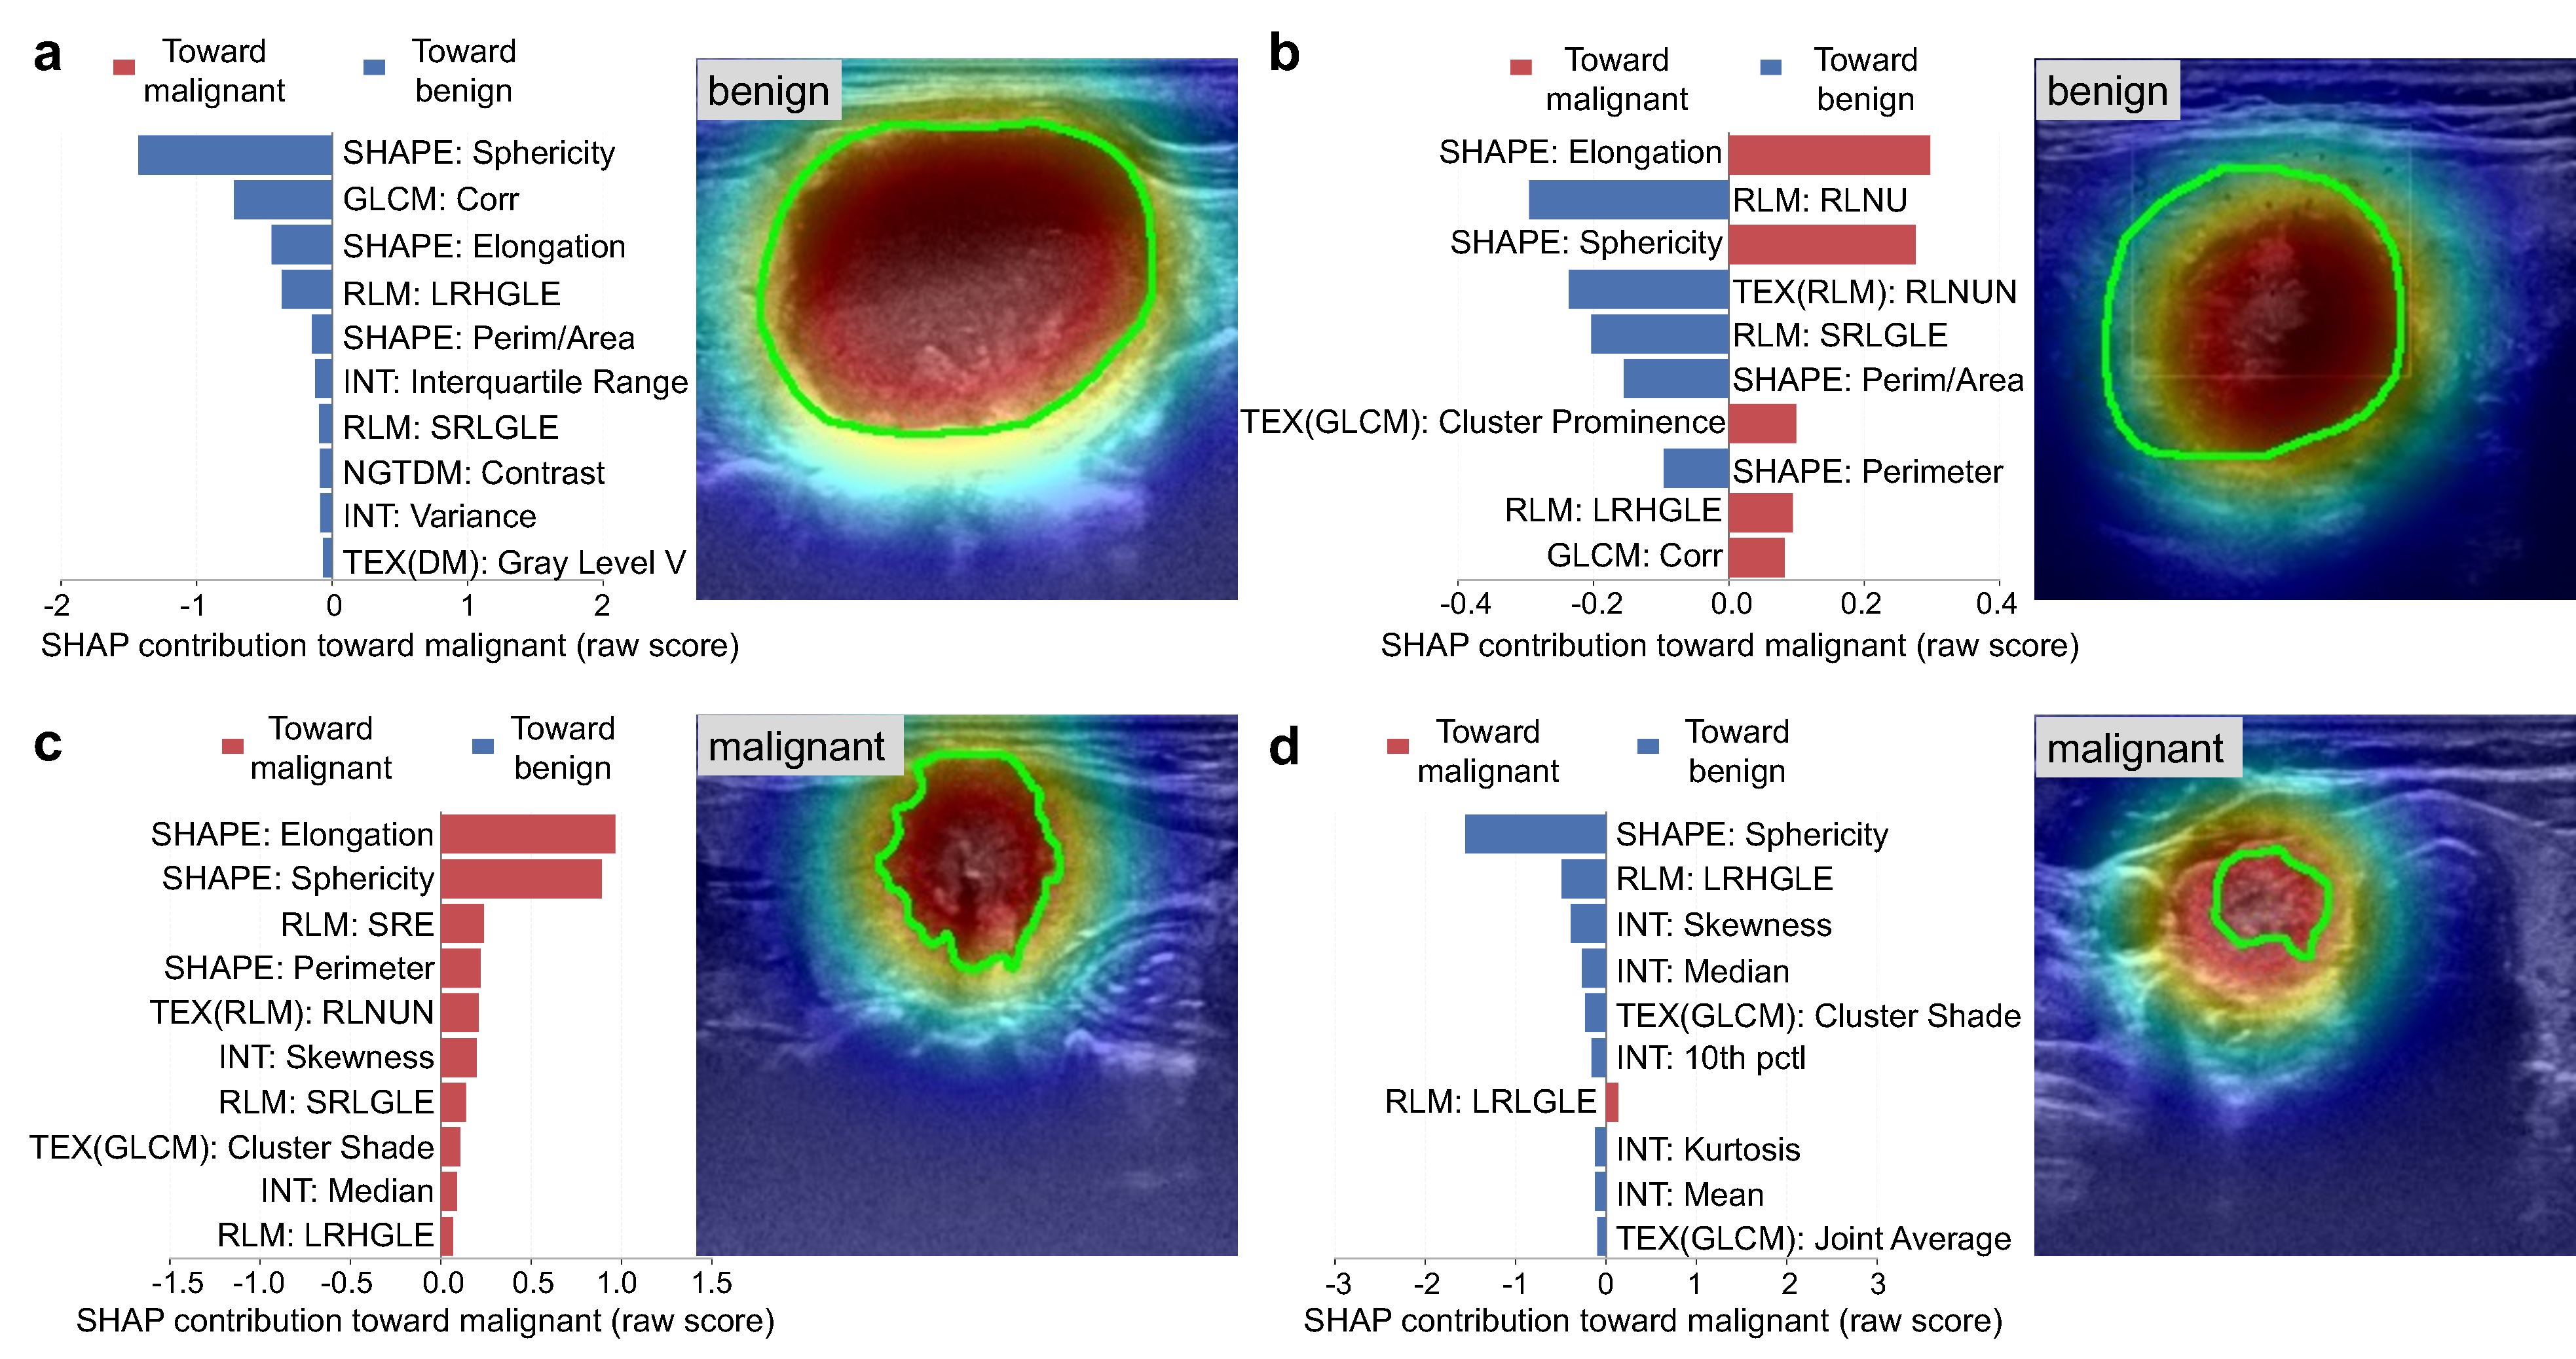
\includegraphics[width=\textwidth,height=0.72\textheight,keepaspectratio]{imgs_sup/BM_cases.pdf}
    \caption{Case-level explanations for thyroid nodule classification. Left, SHAP values for the most influential radiomic features; red and blue indicate contributions towards malignant and benign predictions, respectively. Right, ultrasound images with segmentation contours and Grad-CAM maps from the selected segmentation model. Representative benign and malignant cases with accurate and inaccurate segmentation are shown.}
    \label{fig:BM_cases}
\end{figure}
\clearpage

% Report generation
\begin{figure}[p]
    \centering
    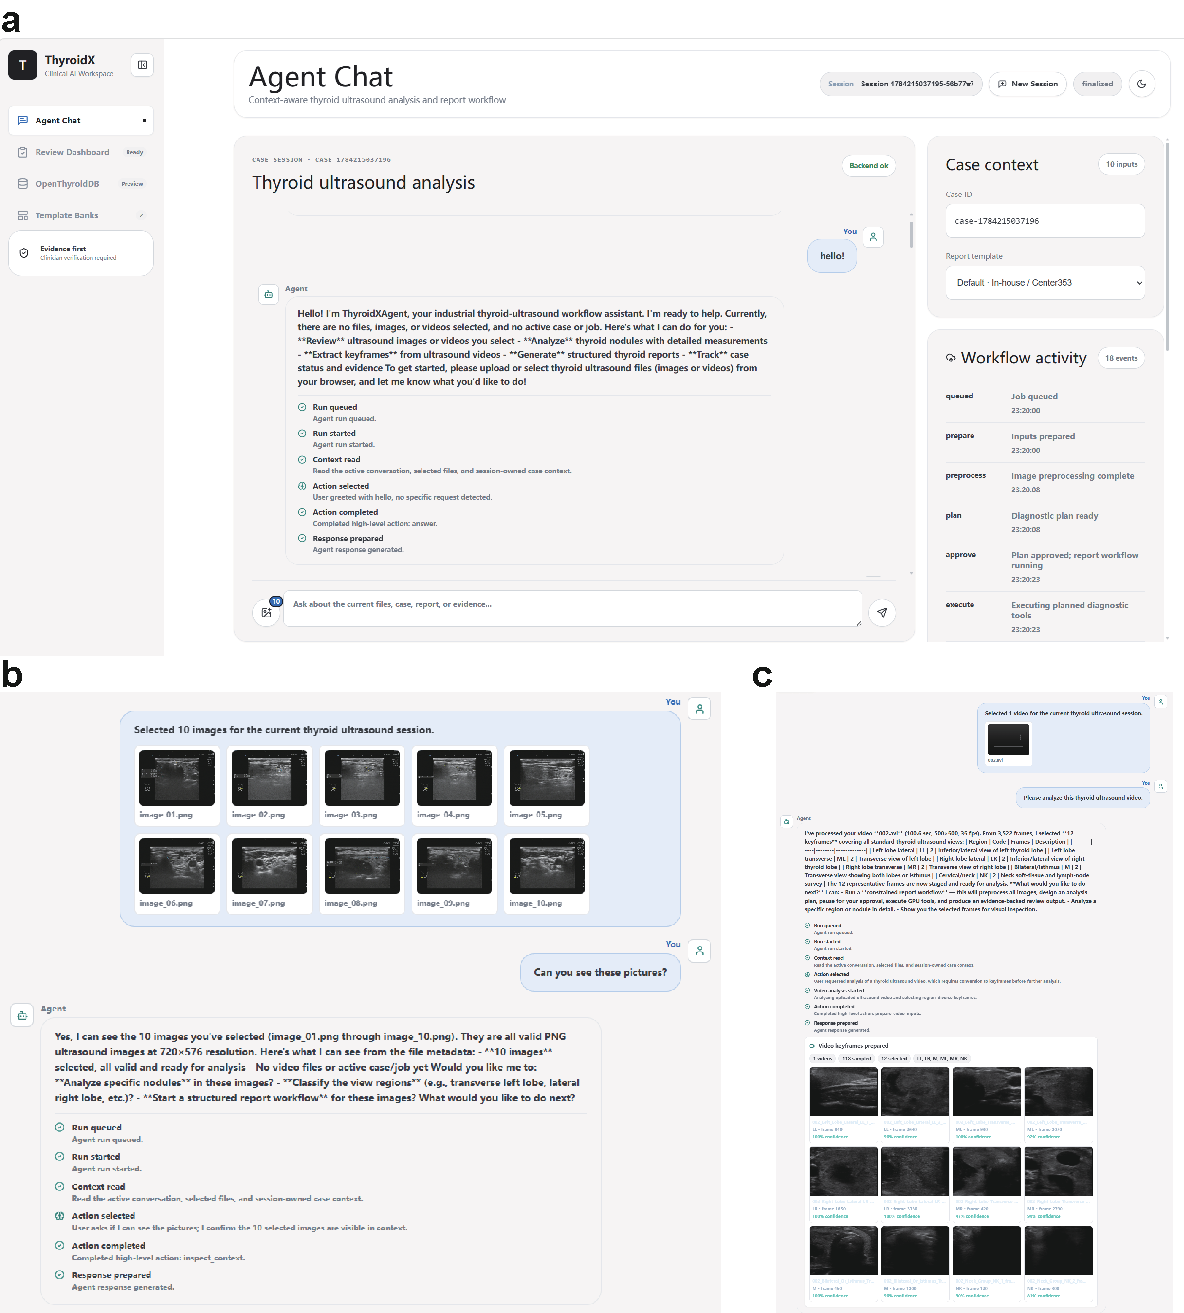
\includegraphics[width=\textwidth,height=0.72\textheight,keepaspectratio]{imgs_sup/ReportGenAgent1.pdf}
    \caption{Multimodal input processing and case interaction in ThyroidXAgent. \textbf{a}, Agent Chat interface for initiating and monitoring case-level thyroid ultrasound analysis, with the case context and workflow activity displayed alongside the conversation. \textbf{b}, Visual perception of case-level, multiview thyroid ultrasound inputs, including image selection, anatomical-region recognition and organization of image-context priors. \textbf{c}, Video-input processing, in which an ultrasound video is sampled into representative frames and organized with anatomical-region predictions and image-context priors for downstream analysis.}
    \label{fig:report_generation_multimodal_interface}
\end{figure}
\clearpage

\begin{figure}[p]
    \centering
    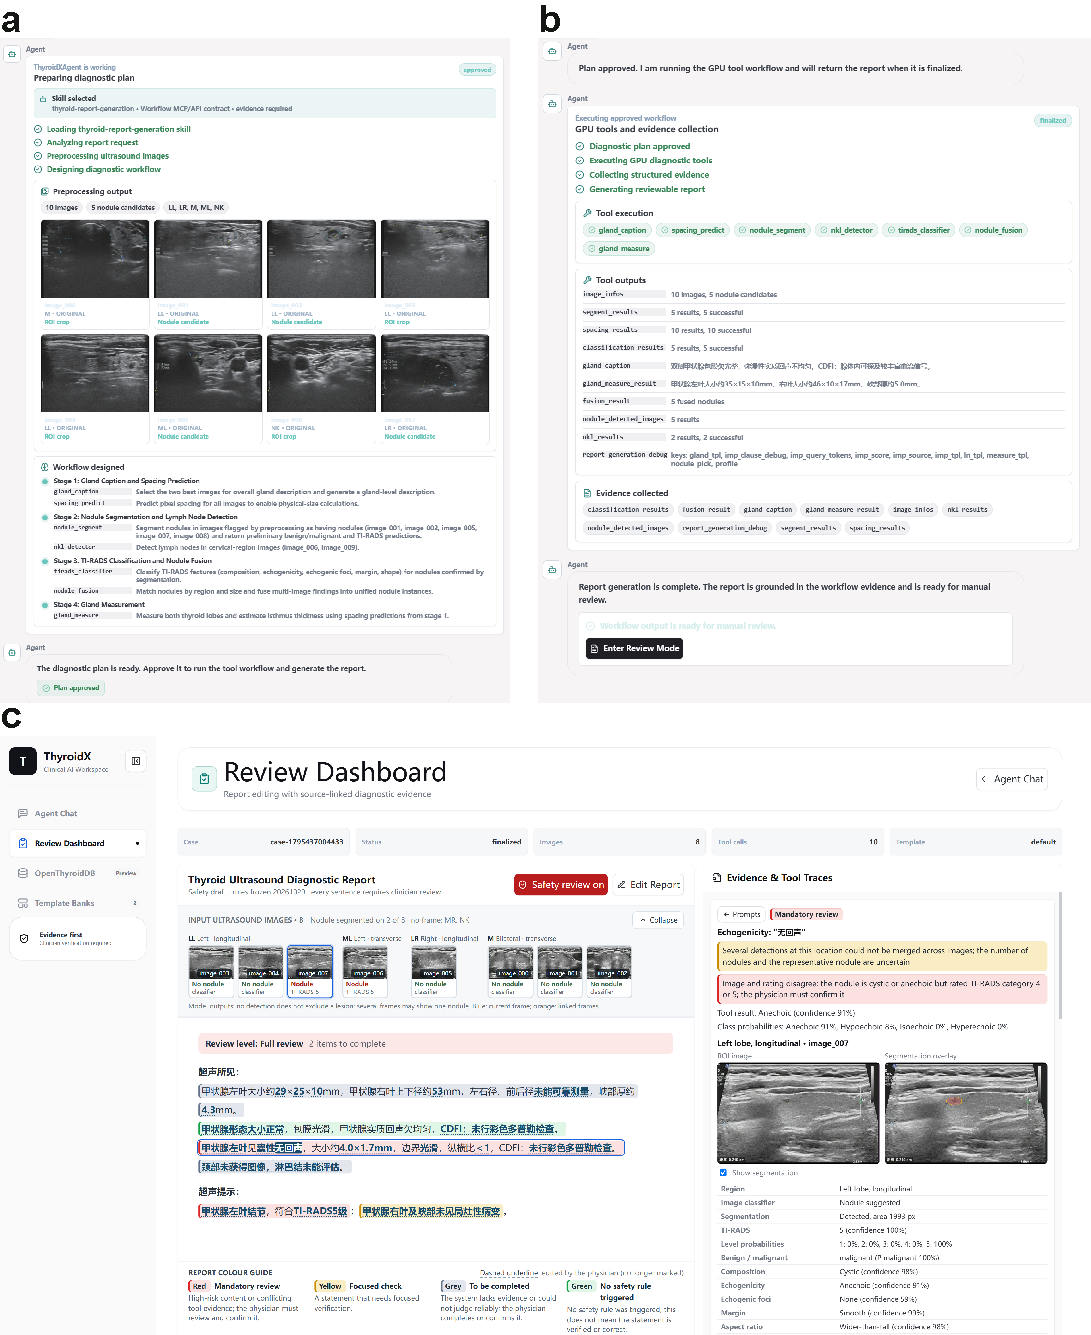
\includegraphics[width=\textwidth,height=0.72\textheight,keepaspectratio]{imgs_sup/ReportGenAgent2.pdf}
    \caption{Planning, tool execution and clinician review in the report-generation workflow. \textbf{a}, Case-specific planning, in which preprocessing outputs, workflow instructions and diagnostic objectives are converted into a staged plan for review and approval. \textbf{b}, Execution after plan approval, showing internal tool calls, intermediate outputs, evidence collection and progression from the approved plan to a reviewable report. \textbf{c}, Report Review Dashboard displaying the generated report alongside source images, structured evidence and tool traces for clinician inspection and editing.}
    \label{fig:report_generation_planning_execution_review}
\end{figure}
\clearpage

\begin{figure}[p]
    \centering
    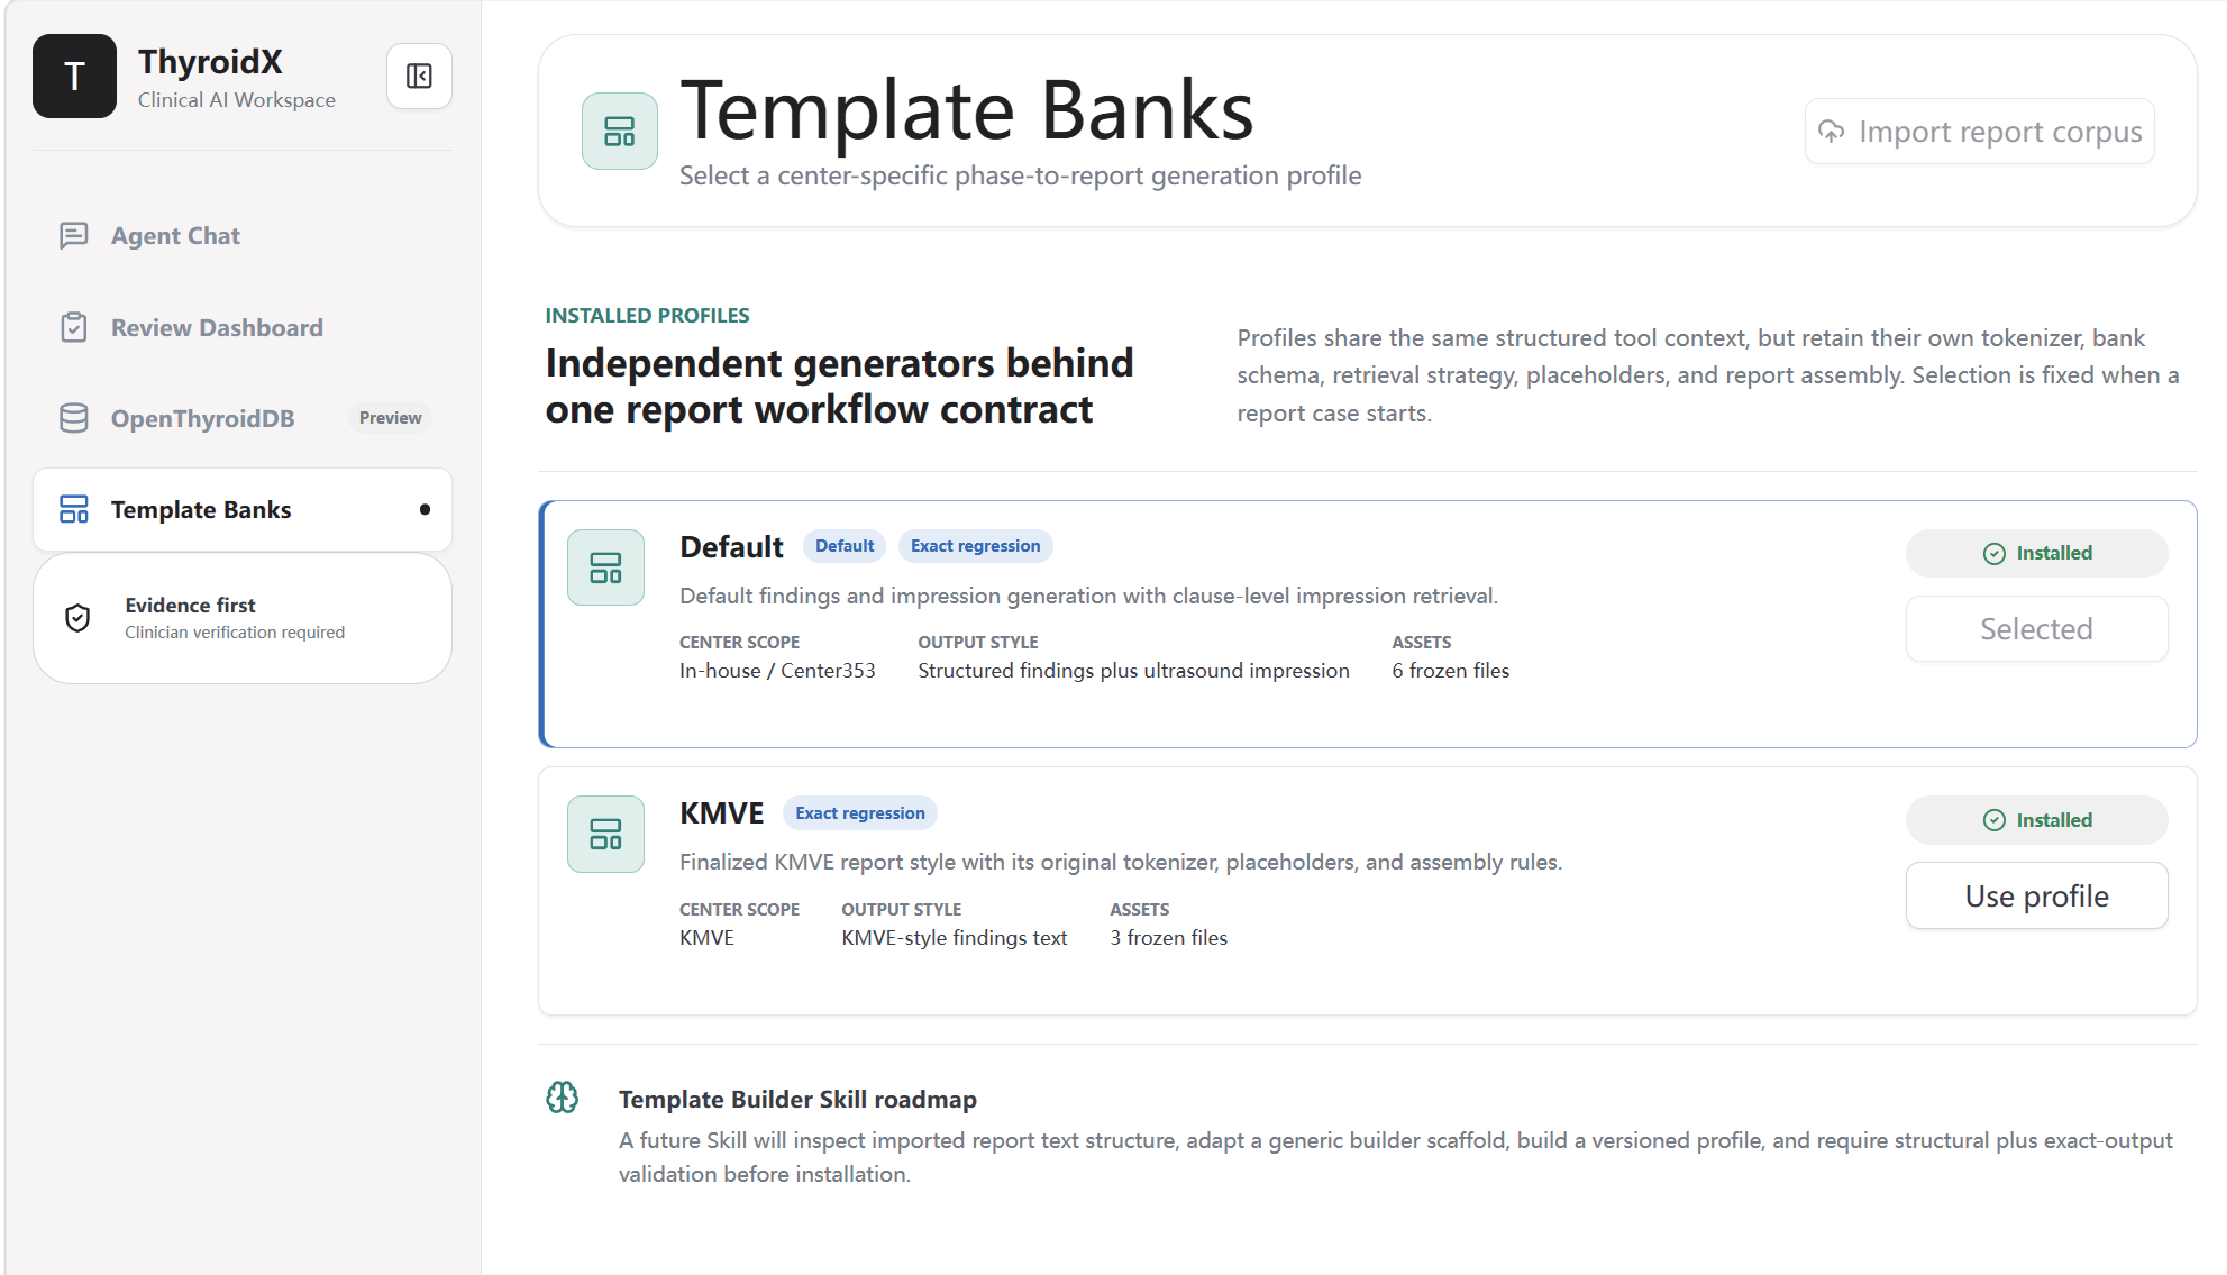
\includegraphics[width=\textwidth,height=0.72\textheight,keepaspectratio]{imgs_sup/ReportGenAgent3.pdf}
    \caption{Template-bank construction for centre-specific report generation. The interface enables users to select an existing centre-specific report-generation profile or import a new report corpus. Generic template-construction scripts derive dataset-specific template banks to support adaptation to additional reporting data.}
    \label{fig:report_generation_template_bank}
\end{figure}
\clearpage

\begin{figure}[p]
    \centering
    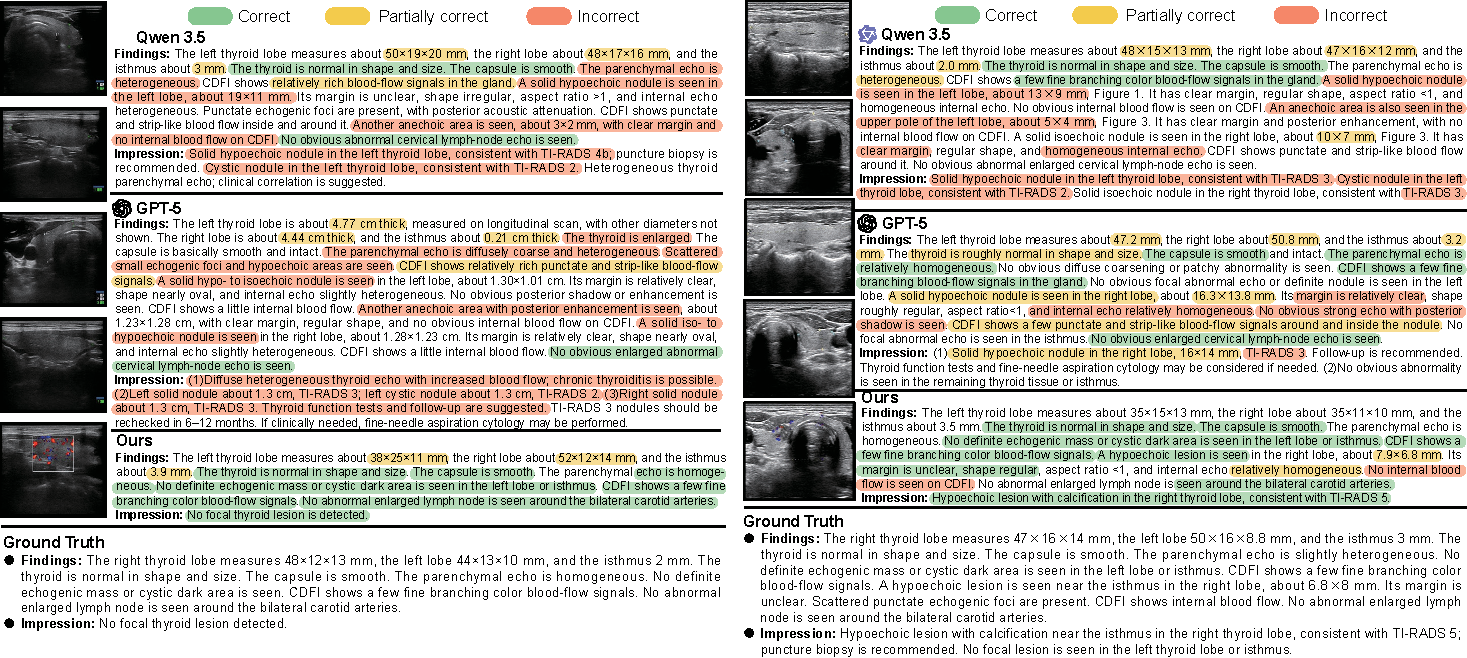
\includegraphics[width=\textwidth,height=0.72\textheight,keepaspectratio]{imgs_sup/RG_CaseReview.pdf}
    \caption{Qualitative comparison of thyroid ultrasound report generation. Representative benign and malignant cases compare reports generated by Qwen 3.5, GPT-5 and ThyroidXAgent with the reference reports. Text spans are annotated as clinically correct, partially correct or incorrect. The malignant example corresponds to Fig.~\ref{fig:reader_study}b; the benign example provides an additional complementary case.}
    \label{fig:RG_CaseReview}
\end{figure}
\clearpage

% ================================================================
% Supplementary Tables: one table per page
% ================================================================
% Framework and data structure
% Supplementary table \label{tab:dataset_summary}
\begin{table}[p]
\centering
\caption{Composition and data splits of the multicentre thyroid ultrasound benchmark. Numbers and percentages show the images contributed by each dataset to the full benchmark (n=37{,}713) and to the training (n=18{,}277), validation (n=850) and test (n=18{,}586) cohorts. DDTI and RJH-7K are independent external test cohorts, and ZJH-8K is a same-centre institutional hold-out test cohort of 6{,}807 images (1{,}068 patients) collected at the hospital that contributed TN3K. DDTI comprises 637 images, of which 349 carry benign-malignant classification labels. ZJH-8K serves as a test set for segmentation and classification; its malignant primary-lesion images additionally provide the development and hold-out sets for malignant-lesion stratification (4{,}028 images, 647 patients; Supplementary Table~\ref{tab:Malignant_images_tasks_performance}).}
\label{tab:dataset_summary}
\renewcommand{\arraystretch}{1.2}
\setlength{\tabcolsep}{4pt}
\footnotesize
\resizebox{\textwidth}{!}{%
\begin{tabular}{llllcccc}
\toprule
\textbf{Dataset} &
\textbf{Task} &
\textbf{Center} &
\textbf{Ultrasound device} &
\textbf{Total} &
\makecell[c]{\textbf{Train}} &
\makecell[c]{\textbf{Valid}} &
\makecell[c]{\textbf{Test}} \\
\midrule
TN3K~\cite{gong2021multi} & \makecell[c]{Segmentation,\\Classification} & \makecell[l]{Zhujiang Hospital,\\Southern Medical\\University, Guangzhou,\\China} & \makecell[l]{GE Logiq E9,\\ARIETTA 850,\\RESONA 70B} & 5{,}347 (14.18\%) & 4{,}633 (25.35\%) & 100 (11.76\%) & 614 (3.30\%) \\
TN5K~\cite{zhang2025tn5000} & \makecell[c]{Segmentation,\\Classification} & \makecell[l]{Cancer Hospital,\\Chinese Academy of\\Medical Sciences,\\Beijing, China} & \makecell[l]{GE Logiq E9,\\GE S7 (5-12 MHz\\or 8-15 MHz)} & 5{,}000 (13.26\%) & 3{,}500 (19.15\%) & 500 (58.82\%) & 1{,}000 (5.38\%) \\
ThyroidXL~\cite{duong2025thyroidxl} & \makecell[c]{Segmentation,\\Classification} & \makecell[l]{Vietnam National\\Hospital of\\Endocrinology,\\Hanoi, Vietnam} & Hitachi Aloka Arietta V70 & 11{,}631 (30.87\%) & 9{,}441 (51.66\%) & 100 (11.76\%) & 2{,}090 (11.25\%) \\
PKTN~\cite{sun2025clip} & Segmentation & \makecell[l]{Peking University\\First Hospital,\\Beijing, China} & -- & 1{,}003 (2.66\%) & 703 (3.85\%) & 150 (17.65\%) & 150 (0.81\%) \\
\midrule
DDTI~\cite{pedraza2015open} & \makecell[c]{Segmentation,\\Classification} & \makecell[l]{IDIME,\\Bogot\'{a}, Colombia} & \makecell[l]{TOSHIBA Nemio 30,\\TOSHIBA Nemio MX\\(12 MHz probe)} & 637 (1.69\%) & -- & -- & \makecell[c]{637 (3.43\%) seg\\349 cls} \\
RJH-7K~\cite{shusharina2021segmentation} & Segmentation & \makecell[l]{Ruijin Hospital,\\Shanghai Jiao Tong\\University School of\\Medicine, Shanghai,\\China} & \makecell[l]{Different machines,\\not specified} & 7{,}288 (19.33\%) & -- & -- & 7{,}288 (39.21\%) \\
ZJH-8K & \makecell[c]{Segmentation,\\Classification} & \makecell[l]{Zhujiang Hospital,\\Southern Medical\\University, Guangzhou,\\China} & -- & 6{,}807 (18.05\%) & -- & -- & 6{,}807 (36.62\%) \\
\bottomrule
\end{tabular}%
}
\end{table}
\clearpage

\clearpage

% Supplementary table \label{tab:dataset_comparison}
\begin{table}[p]
\centering
\caption{Characteristics of public and institutional thyroid ultrasound datasets. Dataset size, data split, file format, task, geographical source and ultrasound scanner information are summarized for the included resources.}
\label{tab:dataset_comparison}
\resizebox{\textwidth}{!}{%
\begin{tabular}{@{}llllllll@{}}
\toprule
\textbf{Dataset} &
\textbf{Dataset Size} &
\textbf{Development/Validation} &
\textbf{Evaluation} &
\textbf{File Format} &
\textbf{Task} &
\textbf{Location} &
\textbf{Ultrasonic Imaging Device} \\
\midrule

TGVideo~\cite{wunderling2017comparison} &
15,186 (16 cases) &
15,186 &
N/A &
\begin{tabular}[c]{@{}l@{}}
Image: DICOM\\
Mask: DICOM
\end{tabular} &
\begin{tabular}[c]{@{}l@{}}
Segmentation\\
Component Development
\end{tabular} &
Germany &
GE Logiq E9 \\

\midrule
DDTI~\cite{pedraza2015open} &
637 &
N/A &
637 &
\begin{tabular}[c]{@{}l@{}}
Image: PNG\\
Mask: PNG\\
Label: CSV
\end{tabular} &
\begin{tabular}[c]{@{}l@{}}
Segmentation\\
Classification
\end{tabular} &
Colombia &
\begin{tabular}[c]{@{}l@{}}
TOSHIBA Nemio 30\\
TOSHIBA Nemio MX
\end{tabular} \\

\midrule
TN3K~\cite{gong2021multi,gong2022less,gong2023thyroid} &
5,347 &
4,733 &
614 &
\begin{tabular}[c]{@{}l@{}}
Image: JPG\\
Mask: JPG\\
Label: CSV
\end{tabular} &
\begin{tabular}[c]{@{}l@{}}
Segmentation\\
Classification\\
Component Development
\end{tabular} &
Guangzhou, China &
\begin{tabular}[c]{@{}l@{}}
GE Logiq E9\\
ARIETTA 850\\
RESONA 70B
\end{tabular} \\

\midrule
TN5K~\cite{zhang2025tn5000} &
5,000 &
4,000 &
1,000 &
\begin{tabular}[c]{@{}l@{}}
Image: JPG\\
Label: XML
\end{tabular} &
\begin{tabular}[c]{@{}l@{}}
Detection\\
Classification
\end{tabular} &
Beijing, China &
\begin{tabular}[c]{@{}l@{}}
GE Logiq E9\\
GE S7
\end{tabular} \\

\midrule
ThyUS2Path~\cite{hou2024ultrasonography} &
8,508 &
5,457 &
3,051 &
\begin{tabular}[c]{@{}l@{}}
Image: JPG\\
Label: CSV
\end{tabular} &
Classification &
Zhejiang, China &
Esaote MyLab (Portable) \\

\midrule
Cine-clip~\cite{stanford2024thyroid} &
\begin{tabular}[c]{@{}l@{}}
17,412 frames\\
192 cases\\
avg. 90 frames/case
\end{tabular} &
N/A &
N/A &
\begin{tabular}[c]{@{}l@{}}
Image: HDF5\\
Label: CSV
\end{tabular} &
\begin{tabular}[c]{@{}l@{}}
Segmentation\\
Classification
\end{tabular} &
California, USA &
N/A \\

\midrule
AHU~\cite{yang2025annotated} &
\begin{tabular}[c]{@{}l@{}}
1,833 cases\\
125,896 images
\end{tabular} &
N/A &
N/A &
\begin{tabular}[c]{@{}l@{}}
Image: JPG\\
Label: Folder-level
\end{tabular} &
Classification &
China (web scraping) &
Heterogeneous \\

\midrule
ThyroidXL~\cite{duong2025thyroidxl} &
11,631 &
9,541 &
2,090 &
\begin{tabular}[c]{@{}l@{}}
Image: PNG\\
Mask: PNG\\
Label: TXT
\end{tabular} &
\begin{tabular}[c]{@{}l@{}}
Segmentation\\
Classification\\
Detection
\end{tabular} &
Vietnam &
Hitachi Aloka Arietta V70 \\

\midrule
PKTN~\cite{sun2025clip} &
1,003 &
N/A &
N/A &
\begin{tabular}[c]{@{}l@{}}
Image: JPG\\
Mask: JPG
\end{tabular} &
Segmentation &
Beijing, China &
N/A \\

\midrule
KMVE~\cite{li_ultrasound_2024} &
\begin{tabular}[c]{@{}l@{}}
2,457 cases\\
4,914 image assignments
\end{tabular} &
\begin{tabular}[c]{@{}l@{}}
1,719 training cases\\
246 validation cases
\end{tabular} &
492 test cases &
\begin{tabular}[c]{@{}l@{}}
Image: JPEG\\
Report: JSON
\end{tabular} &
\begin{tabular}[c]{@{}l@{}}
Report Generation\\
Component Development
\end{tabular} &
Beijing, China &
N/A \\

\midrule
SMU-HMC &
\begin{tabular}[c]{@{}l@{}}
23,955 reports\\
248,194 images
\end{tabular} &
\begin{tabular}[c]{@{}l@{}}
23,555 reports\\
242,210 images
\end{tabular} &
\begin{tabular}[c]{@{}l@{}}
400 reports\\
5,984 images
\end{tabular} &
\begin{tabular}[c]{@{}l@{}}
Image: PNG\\
Report: JSON
\end{tabular} &
\begin{tabular}[c]{@{}l@{}}
Report Generation\\
Component Development
\end{tabular} &
Guangzhou, China &
Heterogeneous \\

\midrule
ZJH-TS &
\begin{tabular}[c]{@{}l@{}}
353 reports\\
4,471 images
\end{tabular} &
N/A &
\begin{tabular}[c]{@{}l@{}}
150 reports\\
2,034 images
\end{tabular} &
\begin{tabular}[c]{@{}l@{}}
Image: PNG\\
Report: JSON
\end{tabular} &
\begin{tabular}[c]{@{}l@{}}
Report Generation\\
External Validation
\end{tabular} &
Guangzhou, China &
Heterogeneous \\

\midrule
TNVideo &
151 cases &
N/A &
145 labelled cases &
Video: AVI &
\begin{tabular}[c]{@{}l@{}}
Segmentation\\
Reader Study
\end{tabular} &
Guangzhou, China &
N/A \\

\bottomrule
\end{tabular}%
}
\end{table}
\clearpage

\clearpage



% Segmentation and classification
% Supplementary table \label{tab:seg_performance}
\begin{table*}[p]
\centering
\begin{threeparttable}

\caption{Cross-dataset generalization for thyroid nodule segmentation. Dice coefficient and 95th-percentile Hausdorff distance (HD95) are reported as point estimates $\pm$ half-widths of 95\% confidence intervals from a cluster bootstrap over patients (1{,}000 resamples; each image formed its own cluster in cohorts without patient identifiers). ZJH-8K: 6{,}807 images (1{,}068 patients).}
\label{tab:seg_performance}

\footnotesize
\setlength{\tabcolsep}{5.5pt}
\renewcommand{\arraystretch}{1.08}

\begin{tabular}{lccccccc}
\toprule
\textbf{Model}
& \textbf{TN3K}
& \textbf{ThyroidXL}
& \textbf{PKTN}
& \textbf{TN5K}
& \textbf{DDTI}
& \textbf{ZJH-8K}
& \textbf{RJH-7K} \\
\midrule
\multicolumn{8}{l}{\textit{Dice (\%) $\uparrow$}} \\
\midrule
TransUnet~\cite{chen2024transunet}
& $81.84 \pm 1.62$
& $85.75 \pm 0.57$
& $76.89 \pm 3.56$
& $78.54 \pm 1.51$
& $76.58 \pm 1.67$
& $76.53 \pm 0.86$
& $84.83 \pm 0.37$ \\
MedSegX~\cite{zhang2025generalist}
& $83.93 \pm 0.79$
& $79.98 \pm 0.36$
& $80.63 \pm 0.42$
& $83.10 \pm 0.48$
& $75.12 \pm 1.68$
& $69.21 \pm 1.00$
& $85.40 \pm 0.18$ \\
MedSAM2~\cite{ma2025medsam2}
& $84.47 \pm 1.02$
& $86.94 \pm 0.36$
& $83.46 \pm 2.60$
& $83.03 \pm 1.29$
& $84.72 \pm 1.26$
& $82.57 \pm 0.82$
& $90.72 \pm 0.21$ \\
UltraFedFM~\cite{jiang2025pretraining}
& $81.18 \pm 1.46$
& $84.70 \pm 0.53$
& $75.31 \pm 1.12$
& $77.13 \pm 1.38$
& $75.57 \pm 1.67$
& $77.56 \pm 0.78$
& $83.10 \pm 0.33$ \\
\rowcolor{lightgray}
\textbf{ThyroidXAgent}
& \textbf{85.69 $\pm$ 1.17}
& \textbf{88.53 $\pm$ 0.42}
& \textbf{85.18 $\pm$ 2.03}
& \textbf{83.88 $\pm$ 1.28}
& \textbf{85.73 $\pm$ 1.10}
& \textbf{88.30 $\pm$ 0.34}
& \textbf{91.77 $\pm$ 0.28} \\

\midrule
\multicolumn{8}{l}{\textit{HD95 (mm) $\downarrow$}} \\
\midrule
TransUnet~\cite{chen2024transunet}
& $27.27 \pm 5.52$
& $22.42 \pm 1.34$
& $26.88 \pm 9.66$
& $22.32 \pm 3.43$
& $17.12 \pm 1.55$
& $16.24 \pm 0.77$
& $18.81 \pm 0.74$ \\
MedSegX~\cite{zhang2025generalist}
& $10.95 \pm 0.64$
& $11.07 \pm 0.32$
& $10.83 \pm 0.70$
& $11.76 \pm 0.76$
& $18.39 \pm 1.65$
& $23.48 \pm 1.04$
& $9.37 \pm 0.18$ \\
MedSAM2~\cite{ma2025medsam2}
& $11.51 \pm 1.53$
& $5.46 \pm 0.44$
& $10.56 \pm 3.64$
& $10.94 \pm 1.12$
& $10.06 \pm 1.21$
& $13.51 \pm 0.83$
& $2.92 \pm 0.17$ \\
UltraFedFM~\cite{jiang2025pretraining}
& $14.98 \pm 2.10$
& $8.10 \pm 0.58$
& $16.08 \pm 1.67$
& $14.96 \pm 1.65$
& $18.12 \pm 1.47$
& $18.57 \pm 0.83$
& $9.06 \pm 0.38$ \\
\rowcolor{lightgray}
\textbf{ThyroidXAgent}
& \textbf{9.42 $\pm$ 1.45}
& \textbf{5.16 $\pm$ 0.53}
& \textbf{9.15 $\pm$ 3.28}
& \textbf{7.14 $\pm$ 1.23}
& \textbf{9.24 $\pm$ 1.06}
& \textbf{10.25 $\pm$ 0.39}
& \textbf{1.88 $\pm$ 0.09} \\

\bottomrule
\end{tabular}
\end{threeparttable}
\end{table*}

\clearpage

% Supplementary table \label{tab:cls_performance}
\begin{table*}[p]
\centering
\begin{threeparttable}

\caption{Cross-dataset generalization for benign-malignant thyroid nodule classification. Area under the receiver operating characteristic curve (AUROC) and area under the precision-recall curve (AUPRC) are reported as point estimates $\pm$ half-widths of 95\% confidence intervals from a cluster bootstrap over patients (1{,}000 resamples; each image formed its own cluster in cohorts without patient identifiers). ZJH-8K: 6{,}807 images (1{,}068 patients).}
\label{tab:cls_performance}

\footnotesize
\setlength{\tabcolsep}{5.5pt}
\renewcommand{\arraystretch}{1.08}

\begin{tabular}{lccccc}
\toprule
\textbf{Method}
& \textbf{TN3K}
& \textbf{ThyroidXL}
& \textbf{TN5K}
& \textbf{DDTI}
& \textbf{ZJH-8K} \\
\midrule
\multicolumn{6}{l}{\textit{AUROC $\uparrow$}} \\
\midrule
ResNet-50~\cite{he2016deep}
& $0.7674 \pm 0.0394$
& $0.9044 \pm 0.0118$
& $0.9322 \pm 0.0168$
& $0.6704 \pm 0.0842$
& $0.8988 \pm 0.0161$ \\
RepViT~\cite{wang2023repvit}
& $0.5556 \pm 0.0463$
& $0.7774 \pm 0.0188$
& $0.6603 \pm 0.0375$
& $0.6162 \pm 0.0804$
& $0.8246 \pm 0.0217$ \\
LSNet~\cite{wang2025lsnet}
& $0.8095 \pm 0.0333$
& $0.9178 \pm 0.0114$
& $0.9091 \pm 0.0201$
& $0.7581 \pm 0.0658$
& $0.8377 \pm 0.0195$ \\
UltraFedFM~\cite{jiang2025pretraining}
& $0.8461 \pm 0.0697$
& $0.9239 \pm 0.0104$
& $0.9298 \pm 0.0175$
& $0.7518 \pm 0.1712$
& $0.8621 \pm 0.0205$ \\
MedGemma~\cite{sellergren2025medgemma}
& $0.8492 \pm 0.0305$
& $0.9371 \pm 0.0095$
& $0.9442 \pm 0.0156$
& \textbf{0.8255 $\pm$ 0.0650}
& $0.9011 \pm 0.0365$ \\
Qwen3-VL-8B-Instruct~\cite{bai2025qwen3}
& $0.8237 \pm 0.0328$
& $0.9050 \pm 0.0115$
& $0.9214 \pm 0.0187$
& $0.7361 \pm 0.0692$
& $0.8397 \pm 0.0338$ \\
GPT-5~\cite{openai2025gpt5systemcard}
& $0.6924 \pm 0.0421$
& $0.7059 \pm 0.0469$
& $0.7737 \pm 0.0996$
& $0.6346 \pm 0.0914$
& $0.6317 \pm 0.0732$ \\
Gemini-2.5-Pro~\cite{comanici_gemini_2025}
& $0.6587 \pm 0.0455$
& $0.6246 \pm 0.0640$
& $0.6873 \pm 0.0691$
& $0.6156 \pm 0.1308$
& $0.6602 \pm 0.0626$ \\
\rowcolor{lightgray}
\textbf{ThyroidXAgent}
& \textbf{0.8714 $\pm$ 0.0299}
& \textbf{0.9680 $\pm$ 0.0066}
& \textbf{0.9584 $\pm$ 0.0152}
& $0.8032 \pm 0.0641$
& \textbf{0.9275 $\pm$ 0.0167} \\
\midrule
\multicolumn{6}{l}{\textit{AUPRC $\uparrow$}} \\
\midrule
ResNet-50~\cite{he2016deep}
& $0.6882 \pm 0.0632$
& $0.8882 \pm 0.0174$
& $0.9674 \pm 0.0268$
& $0.3755 \pm 0.1176$
& $0.9025 \pm 0.0212$ \\
RepViT~\cite{wang2023repvit}
& $0.4275 \pm 0.0528$
& $0.7161 \pm 0.0276$
& $0.8364 \pm 0.0411$
& $0.3924 \pm 0.0933$
& $0.8703 \pm 0.0239$ \\
LSNet~\cite{wang2025lsnet}
& $0.7581 \pm 0.0452$
& $0.9040 \pm 0.0142$
& $0.9551 \pm 0.0134$
& $0.4180 \pm 0.1410$
& $0.8657 \pm 0.0243$ \\
UltraFedFM~\cite{jiang2025pretraining}
& $0.8531 \pm 0.0284$
& $0.9354 \pm 0.0114$
& $0.8422 \pm 0.0421$
& $0.4487 \pm 0.1452$
& $0.9027 \pm 0.0203$ \\
MedGemma~\cite{sellergren2025medgemma}
& $0.8047 \pm 0.0430$
& $0.9201 \pm 0.0139$
& $0.9747 \pm 0.0084$
& $0.5537 \pm 0.1663$
& $0.9079 \pm 0.0114$ \\
Qwen3-VL-8B-Instruct~\cite{bai2025qwen3}
& $0.7617 \pm 0.0511$
& $0.8787 \pm 0.0379$
& $0.9636 \pm 0.0106$
& $0.4112 \pm 0.1415$
& $0.8811 \pm 0.0241$ \\
GPT-5~\cite{openai2025gpt5systemcard}
& $0.6627 \pm 0.0633$
& $0.6237 \pm 0.0666$
& $0.8920 \pm 0.0316$
& $0.3578 \pm 0.1089$
& $0.8120 \pm 0.0541$ \\
Gemini-2.5-Pro~\cite{comanici_gemini_2025}
& $0.6205 \pm 0.0587$
& $0.4914 \pm 0.0841$
& $0.8462 \pm 0.0446$
& $0.3924 \pm 0.1527$
& $0.8197 \pm 0.0613$ \\
\rowcolor{lightgray}
\textbf{ThyroidXAgent}
& \textbf{0.8544 $\pm$ 0.0415}
& \textbf{0.9432 $\pm$ 0.0268}
& \textbf{0.9763 $\pm$ 0.0079}
& \textbf{0.7463 $\pm$ 0.1080}
& \textbf{0.9411 $\pm$ 0.0006} \\
\bottomrule
\end{tabular}
\end{threeparttable}
\end{table*}

\clearpage

% Supplementary table \label{tab:Malignant_images_tasks_performance}
\begin{table*}[p]
\centering
\begin{threeparttable}

\caption{Performance on malignant thyroid lesion stratification. AUROC and AUPRC are reported for central lymph-node metastasis prediction and classification of classic versus follicular-variant papillary thyroid carcinoma (PTC subtype) on the malignant primary-lesion images of ZJH-8K, computed at the patient level. Values are point estimates $\pm$ half-widths of 95\% confidence intervals from 1{,}000 patient-level bootstrap resamples. Top, hold-out test set (801 images, 130 patients); bottom, five-fold cross-validation on the development set (3{,}227 images, 517 patients). Vision-language models were evaluated on the hold-out set only. Em dashes indicate tasks that were not evaluated.}
\label{tab:Malignant_images_tasks_performance}

\footnotesize
\setlength{\tabcolsep}{5.5pt}
\renewcommand{\arraystretch}{1.08}

\begin{tabular}{lcccc}
\toprule
\multirow{2}{*}{\textbf{Method}}
& \multicolumn{2}{c}{\textbf{Lymph Node Metastasis}}
& \multicolumn{2}{c}{\textbf{PTC subtype}} \\
& AUROC $\uparrow$ & AUPRC $\uparrow$ & AUROC $\uparrow$ & AUPRC $\uparrow$ \\
\midrule
\multicolumn{5}{l}{\textit{Hold-out test set (801 images, 130 patients)}} \\
\midrule
RepViT~\cite{wang2023repvit}
& $0.7805 \pm 0.0732$
& $0.7929 \pm 0.0845$
& $0.6638 \pm 0.0821$
& $0.6456 \pm 0.1051$\\
LSNet~\cite{wang2025lsnet}
& $0.6396 \pm 0.0838$
& $0.6585 \pm 0.1113$
& $0.6220 \pm 0.0901$
& $0.6100 \pm 0.1043$\\
UltraFedFM~\cite{jiang2025pretraining}
& $0.8187 \pm 0.0726$
& $0.8252 \pm 0.0972$
& $0.7129 \pm 0.0786$
& $0.7201 \pm 0.0912$\\
MedGemma~\cite{sellergren2025medgemma}
& $0.8388 \pm 0.0562$
& $0.8526 \pm 0.0631$
& $0.7568 \pm 0.0844$
& $0.7239 \pm 0.1102$\\
Qwen3-VL-8B-Instruct~\cite{bai2025qwen3}
& $0.8097 \pm 0.0654$
& $0.8142 \pm 0.0786$
& $0.7071 \pm 0.0821$
& $0.6999 \pm 0.0998$\\
GPT-5~\cite{openai2025gpt5systemcard}
& $0.7911 \pm 0.0653$
& $0.8029 \pm 0.0570$
& $0.3711 \pm 0.1706$
& $0.4638 \pm 0.1347$\\
Gemini-2.5-Pro~\cite{comanici_gemini_2025}
& $0.6063 \pm 0.0955$
& $0.6144 \pm 0.0931$
& $0.4242 \pm 0.1173$
& $0.4586 \pm 0.0893$\\
LLNM-Net~\cite{Shen2025NatCommunLLNM}
& $0.8121 \pm 0.0820$
& $0.8399 \pm 0.0911$
& --
& --\\
Tiger-Model~\cite{Dai2025NatCommunThyroidSubtype}
& --
& --
& $0.7535 \pm 0.1061$
& $0.7741 \pm 0.0989$\\
\rowcolor{lightgray}
\textbf{ThyroidXAgent}
& \textbf{0.8556 $\pm$ 0.0791}
& \textbf{0.8623 $\pm$ 0.0787}
& \textbf{0.7831 $\pm$ 0.0782}
& \textbf{0.7998 $\pm$ 0.0893}\\
\midrule
\multicolumn{5}{l}{\textit{Development set, five-fold cross-validation (3{,}227 images, 517 patients)}} \\
\midrule
RepViT~\cite{wang2023repvit}
& $0.8334 \pm 0.0302$
& $0.8305 \pm 0.0347$
& $0.7005 \pm 0.0471$
& $0.6973 \pm 0.0590$\\
LSNet~\cite{wang2025lsnet}
& $0.7090 \pm 0.0736$
& $0.7083 \pm 0.0925$
& $0.6484 \pm 0.0470$
& $0.6773 \pm 0.0619$\\
UltraFedFM~\cite{jiang2025pretraining}
& $0.8568 \pm 0.0402$
& \textbf{0.8627 $\pm$ 0.0390}
& $0.7812 \pm 0.0393$
& $0.7620 \pm 0.0535$\\
LLNM-Net~\cite{Shen2025NatCommunLLNM}
& $0.8458 \pm 0.0726$
& $0.8369 \pm 0.0875$
& --
& --\\
Tiger-Model~\cite{Dai2025NatCommunThyroidSubtype}
& --
& --
& $0.7877 \pm 0.0466$
& $0.7044 \pm 0.0581$\\
\rowcolor{lightgray}
\textbf{ThyroidXAgent}
& \textbf{0.8797 $\pm$ 0.0285}
& $0.8493 \pm 0.0375$
& \textbf{0.8089 $\pm$ 0.0270}
& \textbf{0.8271 $\pm$ 0.0358}\\
\bottomrule
\end{tabular}
\end{threeparttable}
\end{table*}

\clearpage

\clearpage

% Supplementary table \label{tab:stacked_performance}
\begin{table*}[p]
\centering

\caption{Effects of cumulative training-data integration on segmentation and classification. Models were trained on progressively expanded configurations and evaluated on independent test sets. Segmentation performance is reported as Dice coefficient (\%, $\uparrow$ higher is better) and HD95 (mm, $\downarrow$ lower is better); classification performance as AUROC and AUPRC ($\uparrow$ higher is better). Values are means $\pm$ 95\% confidence intervals across five independent runs. Dashes indicate that the test set was not applicable for the given task. Segmentation training configurations: dataset1 (TN3K), dataset2 (TN3K + ThyroidXL), dataset3 (TN3K + ThyroidXL + PKTN), dataset4 (TN3K + ThyroidXL + PKTN + TN5K). Classification training configurations: dataset1 (TN3K), dataset2 (TN3K + ThyroidXL), dataset3 (TN3K + ThyroidXL + TN5K).}
\label{tab:stacked_performance}

\footnotesize
\setlength{\tabcolsep}{5pt}
\renewcommand{\arraystretch}{1.08}

\resizebox{\textwidth}{!}{%
\begin{tabular}{lccccccc}
\toprule
\diagbox{\textbf{Train}}{\textbf{Test}}
& \textbf{TN3K}
& \textbf{ThyroidXL}
& \textbf{PKTN}
& \textbf{TN5K}
& \textbf{DDTI}
& \textbf{ZJH-8K}
& \textbf{RJH-7K} \\
\midrule
\multicolumn{8}{l}{\textit{Segmentation -- Dice (\%) $\uparrow$}} \\
\midrule
dataset1
& \textbf{82.76 $\pm$ 3.54}
& 81.97 $\pm$ 2.63
& 79.21 $\pm$ 2.71
& 72.18 $\pm$ 5.08
& 78.08 $\pm$ 3.09
& 94.57 $\pm$ 0.43
& 80.77 $\pm$ 0.44 \\
dataset2
& 81.63 $\pm$ 3.81
& 86.84 $\pm$ 1.90
& 81.73 $\pm$ 2.26
& 71.07 $\pm$ 5.35
& 76.72 $\pm$ 3.39
& \textbf{94.85 $\pm$ 0.40}
& 82.38 $\pm$ 0.42 \\
dataset3
& 80.81 $\pm$ 3.82
& 86.00 $\pm$ 2.31
& 81.91 $\pm$ 2.26
& 72.82 $\pm$ 4.91
& 84.81 $\pm$ 2.43
& 94.82 $\pm$ 0.39
& 91.44 $\pm$ 0.15 \\
dataset4
& 81.86 $\pm$ 3.70
& \textbf{86.97 $\pm$ 2.19}
& \textbf{83.28 $\pm$ 2.19}
& \textbf{82.57 $\pm$ 3.46}
& \textbf{84.86 $\pm$ 2.38}
& 94.77 $\pm$ 0.39
& \textbf{91.46 $\pm$ 0.15} \\
\midrule
\multicolumn{8}{l}{\textit{Segmentation -- HD95 (mm) $\downarrow$}} \\
\midrule
dataset1
& \textbf{13.49 $\pm$ 3.83}
& 8.34 $\pm$ 2.34
& 11.73 $\pm$ 3.07
& 11.37 $\pm$ 3.49
& 16.93 $\pm$ 3.12
& 2.30 $\pm$ 0.47
& 11.46 $\pm$ 0.50 \\
dataset2
& 15.92 $\pm$ 4.58
& 4.99 $\pm$ 1.58
& 9.72 $\pm$ 2.71
& 13.64 $\pm$ 4.28
& 18.54 $\pm$ 3.17
& 1.98 $\pm$ 0.41
& 9.65 $\pm$ 0.44 \\
dataset3
& 15.94 $\pm$ 4.34
& 5.46 $\pm$ 1.62
& 10.92 $\pm$ 3.52
& 11.07 $\pm$ 3.28
& 11.97 $\pm$ 3.98
& \textbf{1.93 $\pm$ 0.38}
& \textbf{1.87 $\pm$ 0.07} \\
dataset4
& 17.00 $\pm$ 5.34
& \textbf{4.74 $\pm$ 1.42}
& \textbf{8.89 $\pm$ 2.93}
& \textbf{4.64 $\pm$ 1.43}
& \textbf{9.91 $\pm$ 2.18}
& 2.07 $\pm$ 0.40
& 1.88 $\pm$ 0.07 \\
\midrule
\multicolumn{8}{l}{\textit{Classification -- AUROC $\uparrow$}} \\
\midrule
dataset1
& 0.7666 $\pm$ 0.03
& 0.8713 $\pm$ 0.01
& --
& 0.8272 $\pm$ 0.02
& 0.7244 $\pm$ 0.07
& 0.9924 $\pm$ 0.01
& -- \\
dataset2
& 0.7724 $\pm$ 0.04
& 0.9254 $\pm$ 0.01
& --
& 0.8151 $\pm$ 0.02
& 0.5762 $\pm$ 0.10
& 0.9932 $\pm$ 0.01
& -- \\
dataset3
& \textbf{0.7906 $\pm$ 0.03}
& \textbf{0.9288 $\pm$ 0.01}
& --
& \textbf{0.9515 $\pm$ 0.01}
& \textbf{0.7623 $\pm$ 0.07}
& \textbf{0.9937 $\pm$ 0.01}
& -- \\
\midrule
\multicolumn{8}{l}{\textit{Classification -- AUPRC $\uparrow$}} \\
\midrule
dataset1
& 0.6806 $\pm$ 0.06
& 0.8147 $\pm$ 0.03
& --
& 0.9151 $\pm$ 0.02
& 0.3578 $\pm$ 0.13
& 0.9951 $\pm$ 0.01
& -- \\
dataset2
& \textbf{0.7237 $\pm$ 0.05}
& 0.9140 $\pm$ 0.01
& --
& 0.9074 $\pm$ 0.01
& 0.3190 $\pm$ 0.14
& \textbf{0.9968 $\pm$ 0.01}
& -- \\
dataset3
& 0.7188 $\pm$ 0.05
& \textbf{0.9144 $\pm$ 0.01}
& --
& \textbf{0.9803 $\pm$ 0.01}
& \textbf{0.4029 $\pm$ 0.14}
& 0.9967 $\pm$ 0.01
& -- \\
\bottomrule
\end{tabular}%
}
\end{table*}

\clearpage

% Per-centre segmentation and classification performance on NHC-MISD-TUS
% NHC-MISD-TUS per-centre table \label{tab:gland_dice}
\begin{table}[p]
\centering
\caption{Per-centre Dice similarity coefficient (\%) for thyroid gland segmentation on the NHC-MISD-TUS external test set. Values are reported as point estimates with 95\% confidence intervals. Bold indicates the best result in each row.}
\label{tab:gland_dice}
\footnotesize
\setlength{\tabcolsep}{4pt}
\begin{tabular}{llrrrrr}
\toprule
\multirow{2}{*}{Center} & \multirow{2}{*}{$N$} & \multicolumn{1}{c}{ThyroidXAgent} & \multicolumn{1}{c}{MedSAM2} & \multicolumn{1}{c}{MedSegX} & \multicolumn{1}{c}{TransUNet} & \multicolumn{1}{c}{UltraFedFM} \\
\cmidrule(lr){3-3} \cmidrule(lr){4-4} \cmidrule(lr){5-5} \cmidrule(lr){6-6} \cmidrule(lr){7-7}
 & & Dice (\%) $\uparrow$ & Dice (\%) $\uparrow$ & Dice (\%) $\uparrow$ & Dice (\%) $\uparrow$ & Dice (\%) $\uparrow$ \\
\midrule
\textit{Overall} & 8,721 & 59.28\textsubscript{(58.70, 59.86)} & 56.80\textsubscript{(56.35, 57.24)} & 54.98\textsubscript{(54.57, 55.39)} & 53.56\textsubscript{(53.06, 54.12)} & 33.30\textsubscript{(32.73, 33.88)} \\
\midrule
THYB\_S\_ZJ24 & 1,174 & \textbf{80.64}\textsubscript{(79.84, 81.40)} & 52.96\textsubscript{(51.96, 54.03)} & 50.32\textsubscript{(49.25, 51.42)} & 72.91\textsubscript{(72.03, 73.79)} & 8.49\textsubscript{(7.59, 9.42)} \\
THYB\_S\_EN04 & 949 & \textbf{65.30}\textsubscript{(63.82, 66.78)} & 51.05\textsubscript{(49.46, 52.51)} & 59.83\textsubscript{(58.66, 60.96)} & 59.65\textsubscript{(58.11, 61.15)} & 35.33\textsubscript{(33.81, 36.91)} \\
THYB\_S\_BJ01 & 876 & 61.05\textsubscript{(59.14, 62.88)} & \textbf{61.22}\textsubscript{(59.93, 62.48)} & 51.36\textsubscript{(49.83, 52.83)} & 56.68\textsubscript{(54.95, 58.35)} & 27.42\textsubscript{(25.73, 29.23)} \\
THYB\_S\_SH01 & 832 & 43.33\textsubscript{(41.36, 45.33)} & \textbf{64.88}\textsubscript{(63.37, 66.28)} & 55.60\textsubscript{(54.14, 56.95)} & 42.72\textsubscript{(40.94, 44.52)} & 49.82\textsubscript{(48.11, 51.48)} \\
THYB\_S\_ZJ05 & 694 & \textbf{55.25}\textsubscript{(53.12, 57.40)} & 54.83\textsubscript{(53.19, 56.51)} & 53.77\textsubscript{(52.33, 55.13)} & 50.71\textsubscript{(48.70, 52.55)} & 30.49\textsubscript{(28.66, 32.35)} \\
THYB\_S\_SH05 & 669 & \textbf{61.58}\textsubscript{(59.74, 63.48)} & 59.92\textsubscript{(58.52, 61.38)} & 56.63\textsubscript{(55.27, 57.98)} & 50.26\textsubscript{(48.46, 52.13)} & 34.59\textsubscript{(32.66, 36.40)} \\
THYB\_S\_NX01 & 582 & 52.69\textsubscript{(50.28, 54.89)} & 45.59\textsubscript{(44.00, 47.18)} & 52.80\textsubscript{(51.32, 54.40)} & \textbf{54.11}\textsubscript{(51.83, 56.22)} & 32.64\textsubscript{(30.64, 34.63)} \\
THYB\_S\_ZJ06 & 460 & 48.58\textsubscript{(46.12, 50.98)} & \textbf{62.74}\textsubscript{(60.83, 64.42)} & 55.20\textsubscript{(53.35, 56.97)} & 42.03\textsubscript{(39.70, 44.34)} & 35.19\textsubscript{(32.95, 37.35)} \\
THYB\_S\_QX07 & 289 & \textbf{66.05}\textsubscript{(63.24, 68.91)} & 50.61\textsubscript{(48.09, 53.10)} & 59.57\textsubscript{(57.62, 61.64)} & 62.24\textsubscript{(59.24, 65.06)} & 46.38\textsubscript{(43.64, 49.40)} \\
THYB\_S\_AN01 & 243 & 36.90\textsubscript{(33.32, 40.25)} & \textbf{74.15}\textsubscript{(71.96, 76.34)} & 56.14\textsubscript{(53.14, 59.07)} & 36.30\textsubscript{(33.35, 39.72)} & 60.76\textsubscript{(57.91, 63.56)} \\
THYB\_S\_CQ03 & 238 & \textbf{63.69}\textsubscript{(60.50, 66.62)} & 55.01\textsubscript{(52.63, 57.49)} & 58.52\textsubscript{(56.01, 60.89)} & 46.06\textsubscript{(42.68, 49.56)} & 33.93\textsubscript{(30.82, 37.30)} \\
THYB\_S\_GZ02 & 233 & 59.92\textsubscript{(56.20, 63.38)} & \textbf{62.23}\textsubscript{(60.11, 64.35)} & 55.84\textsubscript{(53.35, 58.40)} & 54.40\textsubscript{(51.00, 58.00)} & 37.71\textsubscript{(34.20, 41.27)} \\
THYB\_S\_JX06 & 215 & 54.16\textsubscript{(50.51, 58.01)} & \textbf{63.46}\textsubscript{(60.77, 65.99)} & 55.71\textsubscript{(52.48, 58.52)} & 45.96\textsubscript{(42.07, 49.54)} & 46.71\textsubscript{(43.30, 50.23)} \\
THYB\_S\_JS02 & 190 & 36.44\textsubscript{(32.39, 40.43)} & \textbf{64.41}\textsubscript{(61.96, 66.78)} & 56.60\textsubscript{(54.36, 58.91)} & 34.57\textsubscript{(31.09, 38.09)} & 50.48\textsubscript{(46.08, 54.64)} \\
THYB\_S\_YN05 & 137 & 55.44\textsubscript{(50.24, 60.32)} & 52.03\textsubscript{(48.59, 55.63)} & \textbf{63.75}\textsubscript{(60.52, 66.75)} & 63.10\textsubscript{(58.34, 67.44)} & 14.28\textsubscript{(10.73, 18.14)} \\
THYB\_S\_EN02 & 120 & \textbf{55.75}\textsubscript{(50.96, 60.59)} & 39.06\textsubscript{(36.22, 42.01)} & 51.87\textsubscript{(48.88, 54.83)} & 38.76\textsubscript{(33.77, 43.55)} & 40.34\textsubscript{(35.64, 44.90)} \\
THYB\_S\_AH04 & 101 & \textbf{65.76}\textsubscript{(59.94, 70.88)} & 52.92\textsubscript{(49.38, 56.65)} & 61.94\textsubscript{(58.10, 65.51)} & 56.38\textsubscript{(50.58, 61.47)} & 47.68\textsubscript{(41.39, 54.39)} \\
THYB\_S\_GS03 & 94 & 50.96\textsubscript{(45.22, 56.84)} & \textbf{59.17}\textsubscript{(54.56, 63.60)} & 51.74\textsubscript{(47.42, 55.76)} & 48.24\textsubscript{(42.53, 53.76)} & 40.09\textsubscript{(34.46, 45.45)} \\
THYB\_S\_FJ03 & 85 & \textbf{66.63}\textsubscript{(60.76, 72.05)} & 46.90\textsubscript{(43.13, 50.64)} & 54.13\textsubscript{(50.57, 57.52)} & 50.83\textsubscript{(44.94, 56.45)} & 36.40\textsubscript{(30.87, 41.92)} \\
THYB\_S\_SD12 & 75 & \textbf{69.59}\textsubscript{(64.15, 74.62)} & 64.10\textsubscript{(60.34, 67.84)} & 59.41\textsubscript{(55.70, 63.10)} & 58.28\textsubscript{(52.76, 63.56)} & 33.57\textsubscript{(27.12, 39.83)} \\
THYB\_S\_JS01 & 72 & \textbf{56.33}\textsubscript{(49.82, 62.97)} & 49.38\textsubscript{(45.18, 53.56)} & 54.34\textsubscript{(50.59, 58.03)} & 49.09\textsubscript{(42.61, 55.51)} & 28.27\textsubscript{(23.18, 33.88)} \\
THYB\_S\_NM02 & 66 & \textbf{57.71}\textsubscript{(52.20, 63.08)} & 52.72\textsubscript{(47.87, 57.77)} & 52.81\textsubscript{(47.81, 57.29)} & 46.24\textsubscript{(40.41, 52.18)} & 36.74\textsubscript{(30.84, 42.37)} \\
THYB\_S\_JL04 & 54 & 43.92\textsubscript{(34.91, 52.81)} & \textbf{56.22}\textsubscript{(50.23, 62.17)} & 55.83\textsubscript{(50.74, 61.29)} & 40.85\textsubscript{(32.13, 49.16)} & 42.49\textsubscript{(34.52, 50.97)} \\
THYB\_S\_SH06 & 43 & 49.75\textsubscript{(41.79, 57.64)} & \textbf{51.33}\textsubscript{(45.78, 56.54)} & 45.09\textsubscript{(37.42, 51.92)} & 46.30\textsubscript{(37.76, 54.02)} & 22.32\textsubscript{(15.88, 29.32)} \\
THYB\_S\_BJ09 & 41 & 54.80\textsubscript{(46.03, 63.29)} & \textbf{55.54}\textsubscript{(49.59, 61.66)} & 55.00\textsubscript{(50.40, 59.85)} & 39.65\textsubscript{(31.89, 47.97)} & 52.67\textsubscript{(44.89, 60.73)} \\
THYB\_S\_SX04 & 41 & \textbf{61.37}\textsubscript{(55.03, 67.56)} & 56.50\textsubscript{(50.56, 62.42)} & 48.79\textsubscript{(42.56, 54.12)} & 44.04\textsubscript{(34.60, 52.15)} & 42.36\textsubscript{(33.90, 51.28)} \\
THYB\_S\_SC06 & 29 & 38.63\textsubscript{(29.91, 48.19)} & \textbf{69.92}\textsubscript{(62.86, 76.12)} & 58.20\textsubscript{(49.69, 65.60)} & 32.00\textsubscript{(25.56, 38.77)} & 59.45\textsubscript{(50.88, 67.48)} \\
THYB\_S\_XJ01 & 25 & \textbf{68.57}\textsubscript{(58.62, 77.48)} & 55.07\textsubscript{(48.48, 61.59)} & 57.03\textsubscript{(50.98, 62.37)} & 60.51\textsubscript{(51.17, 68.75)} & 14.00\textsubscript{(7.83, 21.61)} \\
THYB\_S\_YN01 & 25 & 55.83\textsubscript{(43.67, 66.82)} & \textbf{58.55}\textsubscript{(51.86, 65.06)} & 56.48\textsubscript{(48.32, 64.21)} & 46.59\textsubscript{(35.73, 57.93)} & 29.32\textsubscript{(19.14, 40.82)} \\
THYB\_S\_SD13 & 22 & 69.21\textsubscript{(57.84, 80.57)} & \textbf{72.83}\textsubscript{(63.53, 80.86)} & 63.22\textsubscript{(55.37, 71.01)} & 41.87\textsubscript{(31.62, 52.02)} & 46.04\textsubscript{(34.90, 56.40)} \\
THYB\_S\_GX01 & 19 & \textbf{64.80}\textsubscript{(52.35, 75.87)} & 53.73\textsubscript{(46.83, 61.09)} & 60.04\textsubscript{(51.68, 67.03)} & 61.17\textsubscript{(48.99, 71.80)} & 24.77\textsubscript{(12.11, 38.80)} \\
THYB\_S\_ZJ29 & 16 & \textbf{85.21}\textsubscript{(82.65, 87.63)} & 52.40\textsubscript{(43.77, 61.90)} & 67.08\textsubscript{(59.58, 74.31)} & 47.06\textsubscript{(32.00, 61.91)} & 3.30\textsubscript{(0.48, 7.60)} \\
THYB\_S\_HB07 & 8 & 31.68\textsubscript{(9.84, 58.05)} & \textbf{69.62}\textsubscript{(56.11, 82.55)} & 52.10\textsubscript{(37.92, 62.81)} & 19.55\textsubscript{(0.08, 43.94)} & 29.09\textsubscript{(16.83, 41.56)} \\
THYB\_S\_FJ01 & 2 & \textbf{67.14}\textsubscript{(64.04, 70.23)} & 44.00\textsubscript{(38.25, 49.75)} & 49.95\textsubscript{(43.08, 56.82)} & 45.18\textsubscript{(32.48, 57.89)} & 39.20\textsubscript{(29.38, 49.01)} \\
THYB\_S\_SD14 & 2 & 3.13\textsubscript{(2.55, 3.71)} & 46.73\textsubscript{(36.29, 57.18)} & \textbf{58.38}\textsubscript{(54.22, 62.54)} & 44.78\textsubscript{(31.59, 57.97)} & 37.57\textsubscript{(31.23, 43.91)} \\
\bottomrule
\end{tabular}
\end{table}
\clearpage

\clearpage

% NHC-MISD-TUS per-centre table \label{tab:gland_hd95}
\begin{table}[p]
\centering
\caption{Per-centre 95\% Hausdorff distance (HD95, mm) for thyroid gland segmentation on the NHC-MISD-TUS external test set. Values are reported as point estimates with 95\% confidence intervals. Bold indicates the best result in each row.}
\label{tab:gland_hd95}
\footnotesize
\setlength{\tabcolsep}{4pt}
\begin{tabular}{llrrrrr}
\toprule
\multirow{2}{*}{Center} & \multirow{2}{*}{$N$} & \multicolumn{1}{c}{ThyroidXAgent} & \multicolumn{1}{c}{MedSAM2} & \multicolumn{1}{c}{MedSegX} & \multicolumn{1}{c}{TransUNet} & \multicolumn{1}{c}{UltraFedFM} \\
\cmidrule(lr){3-3} \cmidrule(lr){4-4} \cmidrule(lr){5-5} \cmidrule(lr){6-6} \cmidrule(lr){7-7}
 & & HD95 (mm) $\downarrow$ & HD95 (mm) $\downarrow$ & HD95 (mm) $\downarrow$ & HD95 (mm) $\downarrow$ & HD95 (mm) $\downarrow$ \\
\midrule
\textit{Overall} & 8,721 & 35.83\textsubscript{(35.14, 36.49)} & 65.71\textsubscript{(65.07, 66.38)} & 45.87\textsubscript{(45.36, 46.37)} & 40.65\textsubscript{(39.95, 41.35)} & 58.17\textsubscript{(57.35, 58.99)} \\
\midrule
THYB\_S\_ZJ24 & 1,174 & \textbf{14.74}\textsubscript{(13.90, 15.63)} & 75.31\textsubscript{(73.88, 76.74)} & 64.28\textsubscript{(62.83, 65.85)} & 22.39\textsubscript{(21.43, 23.43)} & 53.71\textsubscript{(50.40, 56.90)} \\
THYB\_S\_EN04 & 949 & \textbf{30.01}\textsubscript{(28.39, 31.72)} & 73.59\textsubscript{(71.54, 75.87)} & 42.31\textsubscript{(40.95, 43.81)} & 34.27\textsubscript{(32.43, 36.13)} & 63.80\textsubscript{(61.88, 65.55)} \\
THYB\_S\_BJ01 & 876 & \textbf{36.67}\textsubscript{(34.70, 38.76)} & 55.12\textsubscript{(53.38, 56.96)} & 41.33\textsubscript{(40.11, 42.83)} & 40.85\textsubscript{(38.94, 43.05)} & 60.27\textsubscript{(57.54, 63.41)} \\
THYB\_S\_SH01 & 832 & 50.89\textsubscript{(48.25, 53.54)} & 55.08\textsubscript{(52.59, 57.51)} & \textbf{39.63}\textsubscript{(38.18, 41.11)} & 51.90\textsubscript{(49.43, 54.61)} & 51.25\textsubscript{(49.37, 53.41)} \\
THYB\_S\_ZJ05 & 694 & \textbf{37.22}\textsubscript{(34.87, 39.57)} & 70.81\textsubscript{(68.16, 73.22)} & 49.93\textsubscript{(48.19, 51.64)} & 40.86\textsubscript{(38.46, 43.25)} & 64.30\textsubscript{(61.86, 67.00)} \\
THYB\_S\_SH05 & 669 & \textbf{36.52}\textsubscript{(34.23, 39.01)} & 58.39\textsubscript{(56.18, 60.42)} & 43.68\textsubscript{(42.20, 45.23)} & 44.98\textsubscript{(42.65, 47.48)} & 67.24\textsubscript{(64.77, 69.87)} \\
THYB\_S\_NX01 & 582 & 39.66\textsubscript{(37.22, 42.54)} & 82.07\textsubscript{(79.47, 84.56)} & 51.93\textsubscript{(49.68, 54.07)} & \textbf{39.06}\textsubscript{(36.74, 41.62)} & 57.51\textsubscript{(54.52, 60.33)} \\
THYB\_S\_ZJ06 & 460 & \textbf{43.86}\textsubscript{(40.98, 47.06)} & 53.93\textsubscript{(51.41, 56.72)} & 44.67\textsubscript{(42.75, 46.81)} & 48.71\textsubscript{(45.68, 51.91)} & 62.98\textsubscript{(60.17, 65.91)} \\
THYB\_S\_QX07 & 289 & \textbf{30.43}\textsubscript{(27.06, 33.67)} & 84.32\textsubscript{(81.13, 87.54)} & 37.11\textsubscript{(35.21, 39.31)} & 34.16\textsubscript{(30.75, 37.53)} & 58.07\textsubscript{(53.90, 61.53)} \\
THYB\_S\_AN01 & 243 & 59.89\textsubscript{(54.84, 65.27)} & 39.11\textsubscript{(35.71, 42.69)} & \textbf{36.76}\textsubscript{(34.09, 39.70)} & 57.02\textsubscript{(52.09, 61.87)} & 42.73\textsubscript{(39.24, 46.33)} \\
THYB\_S\_CQ03 & 238 & \textbf{36.80}\textsubscript{(33.17, 40.64)} & 67.69\textsubscript{(64.19, 71.21)} & 39.40\textsubscript{(36.37, 42.33)} & 49.95\textsubscript{(45.43, 54.40)} & 63.03\textsubscript{(58.68, 67.50)} \\
THYB\_S\_GZ02 & 233 & \textbf{37.00}\textsubscript{(33.22, 40.65)} & 50.49\textsubscript{(47.63, 53.64)} & 39.41\textsubscript{(37.30, 41.67)} & 40.19\textsubscript{(35.91, 44.49)} & 57.61\textsubscript{(53.08, 62.19)} \\
THYB\_S\_JX06 & 215 & 42.43\textsubscript{(38.02, 47.27)} & 54.75\textsubscript{(50.60, 59.00)} & \textbf{37.59}\textsubscript{(35.11, 40.19)} & 48.81\textsubscript{(44.42, 53.58)} & 52.03\textsubscript{(47.75, 56.31)} \\
THYB\_S\_JS02 & 190 & \textbf{49.35}\textsubscript{(44.19, 55.17)} & 52.35\textsubscript{(48.11, 56.54)} & 53.87\textsubscript{(50.49, 57.35)} & 56.88\textsubscript{(51.46, 62.82)} & 52.07\textsubscript{(47.01, 57.13)} \\
THYB\_S\_YN05 & 137 & 37.57\textsubscript{(32.03, 43.12)} & 73.49\textsubscript{(68.84, 77.86)} & \textbf{35.07}\textsubscript{(31.77, 38.50)} & 39.92\textsubscript{(34.22, 46.49)} & 50.39\textsubscript{(41.86, 58.71)} \\
THYB\_S\_EN02 & 120 & \textbf{37.62}\textsubscript{(32.53, 42.62)} & 100.8\textsubscript{(95.9, 105.8)} & 45.67\textsubscript{(42.65, 48.58)} & 44.64\textsubscript{(39.27, 50.38)} & 54.04\textsubscript{(48.46, 59.63)} \\
THYB\_S\_AH04 & 101 & \textbf{25.82}\textsubscript{(20.55, 31.83)} & 70.36\textsubscript{(64.77, 75.45)} & 33.52\textsubscript{(29.78, 37.56)} & 35.53\textsubscript{(29.34, 42.79)} & 52.02\textsubscript{(44.23, 60.59)} \\
THYB\_S\_GS03 & 94 & 44.87\textsubscript{(37.84, 51.56)} & 61.22\textsubscript{(54.74, 67.47)} & \textbf{44.51}\textsubscript{(40.21, 49.25)} & 48.16\textsubscript{(40.83, 55.61)} & 52.29\textsubscript{(45.50, 59.13)} \\
THYB\_S\_FJ03 & 85 & \textbf{27.04}\textsubscript{(21.49, 33.08)} & 83.26\textsubscript{(77.91, 88.32)} & 48.29\textsubscript{(43.55, 53.23)} & 40.21\textsubscript{(34.71, 46.20)} & 57.81\textsubscript{(51.88, 63.89)} \\
THYB\_S\_SD12 & 75 & \textbf{23.80}\textsubscript{(19.40, 28.64)} & 57.62\textsubscript{(52.08, 62.79)} & 36.03\textsubscript{(32.04, 39.97)} & 35.69\textsubscript{(30.37, 41.96)} & 51.62\textsubscript{(43.29, 59.76)} \\
THYB\_S\_JS01 & 72 & \textbf{40.00}\textsubscript{(32.29, 47.62)} & 79.39\textsubscript{(72.78, 85.69)} & 45.34\textsubscript{(40.63, 50.53)} & 40.73\textsubscript{(33.99, 47.88)} & 64.43\textsubscript{(55.62, 73.62)} \\
THYB\_S\_NM02 & 66 & 45.94\textsubscript{(38.55, 53.94)} & 63.04\textsubscript{(56.60, 69.43)} & \textbf{44.14}\textsubscript{(39.41, 49.57)} & 51.02\textsubscript{(42.31, 59.30)} & 62.80\textsubscript{(54.21, 70.52)} \\
THYB\_S\_JL04 & 54 & 53.99\textsubscript{(42.73, 65.60)} & 67.66\textsubscript{(59.00, 76.78)} & \textbf{39.38}\textsubscript{(34.57, 44.49)} & 50.55\textsubscript{(39.81, 61.07)} & 57.53\textsubscript{(46.74, 67.69)} \\
THYB\_S\_SH06 & 43 & 45.77\textsubscript{(34.95, 57.09)} & 63.35\textsubscript{(55.55, 71.99)} & 45.14\textsubscript{(38.78, 51.03)} & \textbf{41.91}\textsubscript{(30.31, 53.31)} & 63.26\textsubscript{(50.44, 76.60)} \\
THYB\_S\_BJ09 & 41 & \textbf{36.63}\textsubscript{(27.94, 47.32)} & 63.20\textsubscript{(55.22, 70.78)} & 42.93\textsubscript{(36.63, 49.75)} & 41.72\textsubscript{(31.74, 52.87)} & 44.38\textsubscript{(34.57, 53.98)} \\
THYB\_S\_SX04 & 41 & \textbf{38.80}\textsubscript{(31.32, 47.14)} & 66.23\textsubscript{(57.04, 75.13)} & 48.62\textsubscript{(44.02, 53.56)} & 53.31\textsubscript{(42.58, 66.15)} & 68.42\textsubscript{(55.93, 82.59)} \\
THYB\_S\_SC06 & 29 & 51.99\textsubscript{(36.85, 66.32)} & 45.67\textsubscript{(35.65, 56.18)} & \textbf{38.52}\textsubscript{(30.69, 46.92)} & 56.62\textsubscript{(43.06, 70.35)} & 43.15\textsubscript{(33.11, 53.56)} \\
THYB\_S\_XJ01 & 25 & \textbf{29.06}\textsubscript{(21.16, 38.25)} & 54.51\textsubscript{(46.58, 63.05)} & 44.52\textsubscript{(37.28, 52.45)} & 44.96\textsubscript{(34.41, 56.69)} & 52.44\textsubscript{(36.21, 68.45)} \\
THYB\_S\_YN01 & 25 & \textbf{35.59}\textsubscript{(22.18, 54.31)} & 62.96\textsubscript{(52.87, 73.71)} & 38.48\textsubscript{(32.35, 44.59)} & 54.30\textsubscript{(37.89, 71.41)} & 66.12\textsubscript{(49.33, 83.02)} \\
THYB\_S\_SD13 & 22 & \textbf{23.75}\textsubscript{(12.47, 36.80)} & 43.51\textsubscript{(30.68, 58.21)} & 36.56\textsubscript{(28.65, 44.41)} & 52.16\textsubscript{(38.57, 65.81)} & 66.39\textsubscript{(52.20, 84.55)} \\
THYB\_S\_GX01 & 19 & 33.19\textsubscript{(22.74, 43.33)} & 78.95\textsubscript{(67.13, 88.94)} & \textbf{29.49}\textsubscript{(22.85, 36.30)} & 38.98\textsubscript{(26.03, 54.00)} & 38.20\textsubscript{(20.84, 60.52)} \\
THYB\_S\_ZJ29 & 16 & \textbf{12.12}\textsubscript{(6.47, 20.65)} & 65.31\textsubscript{(54.30, 76.11)} & 22.34\textsubscript{(17.11, 28.07)} & 38.17\textsubscript{(22.88, 54.66)} & 45.26\textsubscript{(21.23, 69.87)} \\
THYB\_S\_HB07 & 8 & \textbf{30.47}\textsubscript{(7.26, 58.20)} & 44.74\textsubscript{(23.64, 68.97)} & 32.40\textsubscript{(23.17, 45.39)} & 39.33\textsubscript{(7.94, 74.12)} & 80.20\textsubscript{(66.41, 92.63)} \\
THYB\_S\_FJ01 & 2 & 58.89\textsubscript{(23.60, 94.19)} & 75.44\textsubscript{(66.29, 84.60)} & \textbf{33.92}\textsubscript{(27.53, 40.31)} & 47.04\textsubscript{(34.00, 60.08)} & 49.86\textsubscript{(33.24, 66.48)} \\
THYB\_S\_SD14 & 2 & 78.47\textsubscript{(78.16, 78.77)} & 98.68\textsubscript{(81.39, 115.97)} & 55.96\textsubscript{(43.32, 68.59)} & \textbf{34.84}\textsubscript{(19.69, 50.00)} & 40.44\textsubscript{(36.06, 44.82)} \\
\bottomrule
\end{tabular}
\end{table}
\clearpage

\clearpage

% NHC-MISD-TUS per-centre table \label{tab:nodule_dice}
\begin{table}[p]
\centering
\caption{Per-centre Dice similarity coefficient (\%) for thyroid nodule segmentation on the NHC-MISD-TUS external test set. Values are reported as point estimates with 95\% confidence intervals. Bold indicates the best result in each row.}
\label{tab:nodule_dice}
\footnotesize
\setlength{\tabcolsep}{4pt}
\begin{tabular}{llrrrrr}
\toprule
\multirow{2}{*}{Center} & \multirow{2}{*}{$N$} & \multicolumn{1}{c}{ThyroidXAgent} & \multicolumn{1}{c}{MedSAM2} & \multicolumn{1}{c}{MedSegX} & \multicolumn{1}{c}{TransUNet} & \multicolumn{1}{c}{UltraFedFM} \\
\cmidrule(lr){3-3} \cmidrule(lr){4-4} \cmidrule(lr){5-5} \cmidrule(lr){6-6} \cmidrule(lr){7-7}
 & & Dice (\%) $\uparrow$ & Dice (\%) $\uparrow$ & Dice (\%) $\uparrow$ & Dice (\%) $\uparrow$ & Dice (\%) $\uparrow$ \\
\midrule
\textit{Overall} & 6,384 & 82.31\textsubscript{(81.78, 82.83)} & 23.20\textsubscript{(22.58, 23.86)} & 28.82\textsubscript{(28.11, 29.53)} & 72.99\textsubscript{(72.29, 73.68)} & 58.87\textsubscript{(58.04, 59.68)} \\
\midrule
THYB\_S\_EN04 & 946 & \textbf{82.92}\textsubscript{(81.77, 84.00)} & 15.54\textsubscript{(14.29, 16.78)} & 22.25\textsubscript{(20.68, 23.66)} & 74.43\textsubscript{(72.85, 75.95)} & 56.67\textsubscript{(54.69, 58.62)} \\
THYB\_S\_SH01 & 834 & \textbf{88.78}\textsubscript{(88.01, 89.61)} & 39.13\textsubscript{(37.10, 41.01)} & 46.16\textsubscript{(44.13, 48.29)} & 84.48\textsubscript{(83.49, 85.58)} & 71.64\textsubscript{(69.99, 73.33)} \\
THYB\_S\_ZJ05 & 690 & \textbf{82.45}\textsubscript{(81.21, 83.64)} & 15.47\textsubscript{(13.92, 17.01)} & 16.32\textsubscript{(14.69, 17.96)} & 67.34\textsubscript{(65.14, 69.41)} & 55.66\textsubscript{(52.98, 58.07)} \\
THYB\_S\_SH05 & 665 & \textbf{85.53}\textsubscript{(84.17, 86.86)} & 20.11\textsubscript{(18.43, 21.73)} & 29.48\textsubscript{(27.34, 31.47)} & 75.56\textsubscript{(73.63, 77.41)} & 60.40\textsubscript{(57.93, 62.74)} \\
THYB\_S\_NX01 & 557 & \textbf{77.41}\textsubscript{(75.39, 79.40)} & 16.92\textsubscript{(15.32, 18.56)} & 23.51\textsubscript{(21.59, 25.42)} & 68.50\textsubscript{(66.26, 70.91)} & 47.56\textsubscript{(44.76, 50.35)} \\
THYB\_S\_ZJ06 & 460 & \textbf{84.52}\textsubscript{(82.82, 86.14)} & 25.61\textsubscript{(23.25, 27.95)} & 28.94\textsubscript{(26.49, 31.44)} & 75.20\textsubscript{(73.03, 77.38)} & 61.29\textsubscript{(58.63, 63.89)} \\
THYB\_S\_ZJ24 & 321 & \textbf{45.53}\textsubscript{(41.66, 48.73)} & 5.47\textsubscript{(4.61, 6.45)} & 4.17\textsubscript{(3.42, 5.08)} & 20.51\textsubscript{(17.52, 23.78)} & 14.92\textsubscript{(12.15, 17.89)} \\
THYB\_S\_QX07 & 280 & \textbf{85.51}\textsubscript{(83.52, 87.35)} & 22.27\textsubscript{(19.68, 24.88)} & 28.59\textsubscript{(25.55, 31.77)} & 77.89\textsubscript{(74.95, 80.54)} & 68.19\textsubscript{(65.16, 71.49)} \\
THYB\_S\_AN01 & 243 & \textbf{91.60}\textsubscript{(89.81, 92.94)} & 53.29\textsubscript{(49.81, 56.91)} & 61.68\textsubscript{(58.00, 65.00)} & 88.34\textsubscript{(86.28, 90.14)} & 78.19\textsubscript{(75.20, 81.15)} \\
THYB\_S\_CQ03 & 186 & \textbf{82.72}\textsubscript{(79.86, 85.39)} & 18.16\textsubscript{(15.15, 21.46)} & 27.06\textsubscript{(23.17, 31.10)} & 72.57\textsubscript{(68.81, 76.37)} & 55.25\textsubscript{(50.23, 60.01)} \\
THYB\_S\_JS02 & 184 & \textbf{87.67}\textsubscript{(85.58, 89.59)} & 34.39\textsubscript{(30.61, 38.22)} & 35.40\textsubscript{(30.90, 39.94)} & 82.96\textsubscript{(80.24, 85.39)} & 71.70\textsubscript{(67.73, 75.66)} \\
THYB\_S\_JX06 & 167 & \textbf{87.50}\textsubscript{(84.81, 89.82)} & 35.52\textsubscript{(31.67, 39.88)} & 45.33\textsubscript{(40.68, 50.25)} & 83.78\textsubscript{(80.89, 86.39)} & 73.76\textsubscript{(70.40, 77.15)} \\
THYB\_S\_BJ01 & 142 & \textbf{69.73}\textsubscript{(64.15, 74.65)} & 16.56\textsubscript{(13.36, 19.94)} & 21.83\textsubscript{(17.92, 25.72)} & 58.88\textsubscript{(53.18, 64.45)} & 46.92\textsubscript{(41.12, 52.74)} \\
THYB\_S\_EN02 & 107 & \textbf{84.38}\textsubscript{(81.60, 86.98)} & 11.99\textsubscript{(9.13, 15.33)} & 19.36\textsubscript{(15.55, 23.76)} & 73.29\textsubscript{(69.08, 77.46)} & 50.71\textsubscript{(44.52, 57.00)} \\
THYB\_S\_GZ02 & 92 & \textbf{89.21}\textsubscript{(87.74, 90.46)} & 27.23\textsubscript{(22.31, 32.19)} & 30.27\textsubscript{(24.62, 36.27)} & 84.00\textsubscript{(81.49, 86.01)} & 73.15\textsubscript{(68.35, 77.38)} \\
THYB\_S\_GS03 & 91 & \textbf{85.66}\textsubscript{(81.56, 88.93)} & 28.49\textsubscript{(22.48, 34.72)} & 35.22\textsubscript{(28.72, 41.50)} & 78.93\textsubscript{(74.06, 83.12)} & 64.75\textsubscript{(58.31, 70.89)} \\
THYB\_S\_JS01 & 66 & \textbf{85.58}\textsubscript{(81.87, 88.54)} & 13.65\textsubscript{(10.66, 16.77)} & 18.99\textsubscript{(15.28, 23.17)} & 76.18\textsubscript{(70.10, 81.21)} & 58.55\textsubscript{(50.67, 65.99)} \\
THYB\_S\_FJ03 & 64 & \textbf{79.73}\textsubscript{(74.98, 83.85)} & 10.49\textsubscript{(7.58, 13.92)} & 14.62\textsubscript{(10.01, 20.30)} & 64.17\textsubscript{(55.49, 71.69)} & 50.24\textsubscript{(41.88, 59.00)} \\
THYB\_S\_NM02 & 50 & \textbf{83.34}\textsubscript{(75.81, 89.18)} & 21.78\textsubscript{(15.16, 29.35)} & 27.11\textsubscript{(20.14, 34.56)} & 76.31\textsubscript{(67.18, 83.75)} & 61.40\textsubscript{(52.34, 69.28)} \\
THYB\_S\_SH06 & 31 & \textbf{70.85}\textsubscript{(59.24, 79.88)} & 4.60\textsubscript{(3.47, 5.86)} & 8.28\textsubscript{(5.59, 11.59)} & 55.16\textsubscript{(39.98, 68.39)} & 46.54\textsubscript{(33.59, 59.77)} \\
THYB\_S\_AH04 & 30 & \textbf{91.71}\textsubscript{(89.82, 93.31)} & 39.78\textsubscript{(30.88, 48.49)} & 48.60\textsubscript{(37.90, 58.61)} & 84.52\textsubscript{(77.22, 89.78)} & 79.09\textsubscript{(70.70, 84.79)} \\
THYB\_S\_SC06 & 29 & \textbf{90.16}\textsubscript{(88.07, 91.95)} & 44.20\textsubscript{(32.95, 53.60)} & 49.38\textsubscript{(38.45, 58.61)} & 88.29\textsubscript{(85.51, 90.65)} & 76.57\textsubscript{(67.27, 84.35)} \\
THYB\_S\_SX04 & 27 & \textbf{89.20}\textsubscript{(86.29, 91.70)} & 17.84\textsubscript{(12.89, 22.84)} & 16.51\textsubscript{(11.20, 23.50)} & 87.47\textsubscript{(84.52, 89.90)} & 68.19\textsubscript{(57.72, 77.31)} \\
THYB\_S\_BJ09 & 22 & \textbf{86.20}\textsubscript{(81.55, 90.25)} & 30.06\textsubscript{(19.75, 40.78)} & 34.98\textsubscript{(22.71, 47.67)} & 81.62\textsubscript{(74.86, 87.53)} & 70.13\textsubscript{(63.36, 77.01)} \\
THYB\_S\_YN01 & 22 & \textbf{87.24}\textsubscript{(79.41, 92.13)} & 23.20\textsubscript{(13.43, 34.02)} & 28.13\textsubscript{(18.31, 39.88)} & 80.58\textsubscript{(70.28, 87.54)} & 44.07\textsubscript{(29.99, 57.81)} \\
THYB\_S\_SD13 & 18 & \textbf{92.74}\textsubscript{(91.15, 94.06)} & 52.54\textsubscript{(39.34, 64.38)} & 61.58\textsubscript{(48.47, 73.53)} & 90.83\textsubscript{(88.24, 92.78)} & 77.31\textsubscript{(70.93, 82.80)} \\
THYB\_S\_JL04 & 16 & \textbf{81.27}\textsubscript{(67.59, 93.13)} & 36.60\textsubscript{(22.73, 50.94)} & 48.61\textsubscript{(31.53, 65.36)} & 76.87\textsubscript{(62.21, 89.36)} & 70.49\textsubscript{(53.00, 86.26)} \\
THYB\_S\_SD12 & 16 & \textbf{83.71}\textsubscript{(69.71, 93.91)} & 53.71\textsubscript{(39.32, 67.16)} & 62.86\textsubscript{(47.03, 78.03)} & 79.72\textsubscript{(62.56, 93.40)} & 74.86\textsubscript{(58.02, 88.45)} \\
THYB\_S\_YN05 & 12 & \textbf{91.81}\textsubscript{(88.17, 94.81)} & 59.02\textsubscript{(42.58, 71.76)} & 70.91\textsubscript{(51.90, 85.39)} & 91.01\textsubscript{(87.57, 93.88)} & 68.71\textsubscript{(47.83, 85.32)} \\
THYB\_S\_XJ01 & 8 & \textbf{82.71}\textsubscript{(73.69, 90.34)} & 13.18\textsubscript{(4.03, 24.95)} & 14.95\textsubscript{(4.71, 29.10)} & 56.32\textsubscript{(33.11, 79.31)} & 45.53\textsubscript{(20.28, 71.40)} \\
THYB\_S\_GX01 & 4 & \textbf{85.84}\textsubscript{(83.15, 88.54)} & 20.06\textsubscript{(9.70, 30.41)} & 38.09\textsubscript{(22.52, 49.68)} & 84.85\textsubscript{(78.42, 89.87)} & 70.97\textsubscript{(60.58, 83.12)} \\
THYB\_S\_FJ01 & 2 & 79.74\textsubscript{(78.18, 81.31)} & 6.47\textsubscript{(4.46, 8.48)} & 12.32\textsubscript{(8.26, 16.37)} & \textbf{81.94}\textsubscript{(77.73, 86.14)} & 46.04\textsubscript{(36.60, 55.49)} \\
THYB\_S\_HB07 & 2 & 21.28\textsubscript{(18.58, 23.99)} & 1.90\textsubscript{(1.48, 2.31)} & 1.86\textsubscript{(1.61, 2.11)} & \textbf{23.49}\textsubscript{(0.00, 46.97)} & 17.79\textsubscript{(11.76, 23.82)} \\
\bottomrule
\end{tabular}
\end{table}
\clearpage

\clearpage

% NHC-MISD-TUS per-centre table \label{tab:nodule_hd95}
\begin{table}[p]
\centering
\caption{Per-centre 95\% Hausdorff distance (HD95, mm) for thyroid nodule segmentation on the NHC-MISD-TUS external test set. Values are reported as point estimates with 95\% confidence intervals. Bold indicates the best result in each row.}
\label{tab:nodule_hd95}
\footnotesize
\setlength{\tabcolsep}{4pt}
\begin{tabular}{llrrrrr}
\toprule
\multirow{2}{*}{Center} & \multirow{2}{*}{$N$} & \multicolumn{1}{c}{ThyroidXAgent} & \multicolumn{1}{c}{MedSAM2} & \multicolumn{1}{c}{MedSegX} & \multicolumn{1}{c}{TransUNet} & \multicolumn{1}{c}{UltraFedFM} \\
\cmidrule(lr){3-3} \cmidrule(lr){4-4} \cmidrule(lr){5-5} \cmidrule(lr){6-6} \cmidrule(lr){7-7}
 & & HD95 (mm) $\downarrow$ & HD95 (mm) $\downarrow$ & HD95 (mm) $\downarrow$ & HD95 (mm) $\downarrow$ & HD95 (mm) $\downarrow$ \\
\midrule
\textit{Overall} & 6,384 & 9.41\textsubscript{(8.89, 9.93)} & 101.2\textsubscript{(100.2, 102.0)} & 86.96\textsubscript{(86.08, 87.84)} & 10.62\textsubscript{(10.14, 11.12)} & 27.04\textsubscript{(26.28, 27.75)} \\
\midrule
THYB\_S\_EN04 & 946 & \textbf{6.95}\textsubscript{(6.05, 7.91)} & 113.0\textsubscript{(111.0, 114.9)} & 91.23\textsubscript{(89.41, 92.99)} & 9.27\textsubscript{(8.31, 10.37)} & 33.50\textsubscript{(31.47, 35.76)} \\
THYB\_S\_SH01 & 834 & \textbf{6.41}\textsubscript{(5.50, 7.36)} & 79.94\textsubscript{(77.11, 82.81)} & 65.42\textsubscript{(63.21, 67.68)} & 8.32\textsubscript{(7.35, 9.27)} & 21.31\textsubscript{(19.64, 22.92)} \\
THYB\_S\_ZJ05 & 690 & \textbf{5.00}\textsubscript{(4.31, 5.76)} & 108.5\textsubscript{(106.1, 110.6)} & 106.8\textsubscript{(104.6, 109.0)} & 7.73\textsubscript{(6.88, 8.61)} & 21.22\textsubscript{(19.59, 23.13)} \\
THYB\_S\_SH05 & 665 & \textbf{7.60}\textsubscript{(6.34, 8.89)} & 101.8\textsubscript{(99.4, 104.1)} & 81.02\textsubscript{(78.74, 83.33)} & 10.17\textsubscript{(8.84, 11.51)} & 28.23\textsubscript{(25.93, 30.37)} \\
THYB\_S\_NX01 & 557 & \textbf{12.95}\textsubscript{(10.96, 14.86)} & 112.7\textsubscript{(110.1, 115.1)} & 92.51\textsubscript{(89.99, 94.97)} & 13.02\textsubscript{(11.18, 14.80)} & 30.17\textsubscript{(27.56, 32.82)} \\
THYB\_S\_ZJ06 & 460 & \textbf{7.62}\textsubscript{(6.22, 9.24)} & 92.99\textsubscript{(90.07, 95.87)} & 88.02\textsubscript{(85.09, 91.28)} & 10.88\textsubscript{(9.34, 12.66)} & 26.09\textsubscript{(23.54, 28.75)} \\
THYB\_S\_ZJ24 & 321 & 45.03\textsubscript{(39.74, 50.67)} & 142.9\textsubscript{(139.7, 145.9)} & 140.9\textsubscript{(137.7, 143.8)} & \textbf{30.45}\textsubscript{(26.09, 34.77)} & 45.71\textsubscript{(40.11, 51.74)} \\
THYB\_S\_QX07 & 280 & \textbf{6.69}\textsubscript{(5.08, 8.55)} & 110.2\textsubscript{(106.4, 113.9)} & 85.79\textsubscript{(82.50, 89.13)} & 8.11\textsubscript{(6.54, 10.16)} & 22.53\textsubscript{(19.71, 25.68)} \\
THYB\_S\_AN01 & 243 & \textbf{4.70}\textsubscript{(3.51, 6.11)} & 60.30\textsubscript{(55.67, 64.85)} & 49.32\textsubscript{(45.45, 53.68)} & 7.19\textsubscript{(5.65, 9.00)} & 16.62\textsubscript{(14.15, 19.21)} \\
THYB\_S\_CQ03 & 186 & \textbf{8.81}\textsubscript{(5.97, 12.38)} & 105.0\textsubscript{(100.0, 109.4)} & 81.35\textsubscript{(77.26, 85.23)} & 12.51\textsubscript{(9.28, 16.26)} & 33.57\textsubscript{(28.12, 38.94)} \\
THYB\_S\_JS02 & 184 & \textbf{6.68}\textsubscript{(4.75, 8.90)} & 80.55\textsubscript{(75.49, 85.50)} & 84.81\textsubscript{(78.76, 90.71)} & 8.78\textsubscript{(6.74, 10.90)} & 24.40\textsubscript{(20.23, 28.77)} \\
THYB\_S\_JX06 & 167 & \textbf{7.25}\textsubscript{(5.01, 9.88)} & 82.29\textsubscript{(76.67, 87.66)} & 63.70\textsubscript{(58.48, 68.68)} & 9.18\textsubscript{(6.44, 12.50)} & 20.12\textsubscript{(16.76, 23.56)} \\
THYB\_S\_BJ01 & 142 & 20.72\textsubscript{(15.43, 26.10)} & 101.8\textsubscript{(96.3, 107.7)} & 92.30\textsubscript{(87.28, 97.40)} & \textbf{20.10}\textsubscript{(15.47, 25.01)} & 34.87\textsubscript{(29.55, 40.13)} \\
THYB\_S\_EN02 & 107 & \textbf{4.49}\textsubscript{(3.07, 6.59)} & 128.9\textsubscript{(123.9, 133.4)} & 92.21\textsubscript{(87.64, 96.59)} & 8.45\textsubscript{(6.20, 11.49)} & 29.38\textsubscript{(24.47, 34.60)} \\
THYB\_S\_GZ02 & 92 & \textbf{4.51}\textsubscript{(3.43, 5.77)} & 84.00\textsubscript{(78.53, 89.58)} & 81.50\textsubscript{(74.63, 88.26)} & 7.53\textsubscript{(5.65, 9.73)} & 17.57\textsubscript{(13.41, 22.16)} \\
THYB\_S\_GS03 & 91 & \textbf{7.80}\textsubscript{(4.49, 11.81)} & 89.69\textsubscript{(81.70, 97.29)} & 75.21\textsubscript{(68.30, 82.38)} & 8.70\textsubscript{(5.54, 12.57)} & 24.98\textsubscript{(19.70, 31.13)} \\
THYB\_S\_JS01 & 66 & \textbf{5.69}\textsubscript{(3.49, 8.71)} & 111.8\textsubscript{(106.2, 117.2)} & 94.67\textsubscript{(89.47, 99.84)} & 9.84\textsubscript{(6.27, 14.06)} & 27.35\textsubscript{(19.68, 35.58)} \\
THYB\_S\_FJ03 & 64 & \textbf{6.99}\textsubscript{(3.86, 10.72)} & 115.9\textsubscript{(109.6, 122.4)} & 107.7\textsubscript{(100.0, 115.2)} & 8.87\textsubscript{(5.71, 12.92)} & 22.36\textsubscript{(16.53, 28.70)} \\
THYB\_S\_NM02 & 50 & 6.75\textsubscript{(3.95, 10.41)} & 95.61\textsubscript{(85.83, 104.48)} & 82.78\textsubscript{(75.37, 90.43)} & \textbf{6.49}\textsubscript{(4.04, 9.79)} & 21.73\textsubscript{(16.43, 27.52)} \\
THYB\_S\_SH06 & 31 & 16.01\textsubscript{(6.79, 25.90)} & 115.0\textsubscript{(110.3, 120.7)} & 94.85\textsubscript{(88.68, 100.91)} & \textbf{7.08}\textsubscript{(3.20, 12.90)} & 28.90\textsubscript{(17.04, 42.21)} \\
THYB\_S\_AH04 & 30 & \textbf{3.09}\textsubscript{(2.14, 4.32)} & 81.37\textsubscript{(70.67, 92.67)} & 66.34\textsubscript{(54.18, 78.80)} & 9.13\textsubscript{(4.11, 16.74)} & 18.64\textsubscript{(11.53, 27.65)} \\
THYB\_S\_SC06 & 29 & \textbf{4.72}\textsubscript{(2.94, 6.80)} & 71.23\textsubscript{(58.43, 85.23)} & 61.37\textsubscript{(51.00, 72.75)} & 5.60\textsubscript{(3.63, 7.90)} & 20.14\textsubscript{(10.14, 31.55)} \\
THYB\_S\_SX04 & 27 & \textbf{3.54}\textsubscript{(2.39, 4.80)} & 106.5\textsubscript{(98.0, 114.6)} & 108.8\textsubscript{(98.9, 118.0)} & 4.05\textsubscript{(3.12, 5.09)} & 25.37\textsubscript{(14.31, 39.60)} \\
THYB\_S\_BJ09 & 22 & \textbf{5.56}\textsubscript{(3.29, 8.33)} & 85.51\textsubscript{(71.97, 98.12)} & 77.91\textsubscript{(63.39, 92.08)} & 7.06\textsubscript{(3.88, 11.19)} & 18.84\textsubscript{(11.45, 26.82)} \\
THYB\_S\_YN01 & 22 & \textbf{4.61}\textsubscript{(2.12, 8.49)} & 96.72\textsubscript{(83.10, 109.97)} & 73.60\textsubscript{(64.25, 81.65)} & 4.98\textsubscript{(3.42, 6.90)} & 40.06\textsubscript{(27.32, 54.75)} \\
THYB\_S\_SD13 & 18 & \textbf{3.32}\textsubscript{(2.22, 4.57)} & 61.73\textsubscript{(47.66, 76.68)} & 45.00\textsubscript{(32.04, 58.04)} & 4.51\textsubscript{(2.74, 6.60)} & 21.77\textsubscript{(15.46, 28.42)} \\
THYB\_S\_JL04 & 16 & 14.24\textsubscript{(2.17, 31.43)} & 88.05\textsubscript{(70.97, 104.04)} & 58.06\textsubscript{(41.17, 75.76)} & \textbf{12.51}\textsubscript{(3.43, 23.13)} & 16.36\textsubscript{(6.05, 28.72)} \\
THYB\_S\_SD12 & 16 & 9.76\textsubscript{(3.28, 17.71)} & 57.71\textsubscript{(38.35, 78.90)} & 50.35\textsubscript{(31.21, 71.00)} & \textbf{8.08}\textsubscript{(2.22, 15.94)} & 18.16\textsubscript{(7.70, 30.26)} \\
THYB\_S\_YN05 & 12 & \textbf{3.22}\textsubscript{(2.05, 4.34)} & 61.17\textsubscript{(44.75, 80.17)} & 38.97\textsubscript{(24.66, 57.04)} & 4.86\textsubscript{(2.25, 9.08)} & 13.71\textsubscript{(6.45, 21.71)} \\
THYB\_S\_XJ01 & 8 & \textbf{6.99}\textsubscript{(1.71, 16.39)} & 111.3\textsubscript{(92.8, 131.6)} & 99.22\textsubscript{(85.22, 115.90)} & 20.73\textsubscript{(4.35, 42.34)} & 24.55\textsubscript{(5.64, 47.07)} \\
THYB\_S\_GX01 & 4 & 5.57\textsubscript{(3.00, 8.47)} & 101.0\textsubscript{(81.2, 123.7)} & 78.07\textsubscript{(56.31, 92.33)} & \textbf{5.12}\textsubscript{(2.62, 8.46)} & 15.24\textsubscript{(6.58, 25.12)} \\
THYB\_S\_FJ01 & 2 & 8.32\textsubscript{(4.00, 12.65)} & 112.3\textsubscript{(104.0, 120.7)} & 86.49\textsubscript{(73.93, 99.04)} & \textbf{4.41}\textsubscript{(2.83, 6.00)} & 56.71\textsubscript{(26.29, 87.13)} \\
THYB\_S\_HB07 & 2 & 30.80\textsubscript{(18.03, 43.57)} & 109.0\textsubscript{(98.6, 119.4)} & 104.4\textsubscript{(95.2, 113.5)} & \textbf{4.70}\textsubscript{(0.00, 9.39)} & 19.30\textsubscript{(8.60, 30.00)} \\
\bottomrule
\end{tabular}
\end{table}
\clearpage

\clearpage

% NHC-MISD-TUS per-centre table \label{tab:binary_auroc}
\begin{table}[p]
\centering
\caption{Per-centre AUROC for benign versus malignant thyroid nodule classification on the NHC-MISD-TUS external test set. Values are reported as point estimates with 95\% confidence intervals. Bold indicates the best result in each row.}
\label{tab:binary_auroc}
\footnotesize
\setlength{\tabcolsep}{4pt}
\begin{tabular}{llrrrr}
\toprule
\multirow{2}{*}{Center} & \multirow{2}{*}{$N$} & \multicolumn{1}{c}{ThyroidXAgent} & \multicolumn{1}{c}{BiomedCLIP} & \multicolumn{1}{c}{MedSigLIP} & \multicolumn{1}{c}{UltraFedFM} \\
\cmidrule(lr){3-3} \cmidrule(lr){4-4} \cmidrule(lr){5-5} \cmidrule(lr){6-6}
 & & AUROC $\uparrow$ & AUROC $\uparrow$ & AUROC $\uparrow$ & AUROC $\uparrow$ \\
\midrule
\textit{Overall} & 4,999 & 0.819\textsubscript{(0.808, 0.831)} & 0.434\textsubscript{(0.418, 0.450)} & 0.520\textsubscript{(0.503, 0.535)} & 0.436\textsubscript{(0.420, 0.452)} \\
\midrule
THYB\_S\_SH01 & 792 & \textbf{0.896}\textsubscript{(0.873, 0.916)} & 0.327\textsubscript{(0.290, 0.368)} & 0.552\textsubscript{(0.517, 0.594)} & 0.331\textsubscript{(0.295, 0.368)} \\
THYB\_S\_ZJ05 & 647 & \textbf{0.811}\textsubscript{(0.773, 0.844)} & 0.526\textsubscript{(0.480, 0.576)} & 0.586\textsubscript{(0.546, 0.627)} & 0.494\textsubscript{(0.455, 0.533)} \\
THYB\_S\_EN04 & 626 & \textbf{0.846}\textsubscript{(0.808, 0.876)} & 0.345\textsubscript{(0.289, 0.404)} & 0.538\textsubscript{(0.472, 0.597)} & 0.528\textsubscript{(0.476, 0.584)} \\
THYB\_S\_SH05 & 539 & \textbf{0.719}\textsubscript{(0.672, 0.758)} & 0.331\textsubscript{(0.280, 0.381)} & 0.543\textsubscript{(0.492, 0.595)} & 0.370\textsubscript{(0.324, 0.423)} \\
THYB\_S\_ZJ06 & 452 & \textbf{0.811}\textsubscript{(0.768, 0.849)} & 0.468\textsubscript{(0.412, 0.520)} & 0.594\textsubscript{(0.541, 0.651)} & 0.539\textsubscript{(0.486, 0.592)} \\
THYB\_S\_QX07 & 279 & \textbf{0.870}\textsubscript{(0.814, 0.917)} & 0.457\textsubscript{(0.381, 0.537)} & 0.630\textsubscript{(0.534, 0.711)} & 0.428\textsubscript{(0.338, 0.520)} \\
THYB\_S\_ZJ24 & 269 & 0.590\textsubscript{(0.346, 0.832)} & 0.412\textsubscript{(0.270, 0.544)} & \textbf{0.673}\textsubscript{(0.493, 0.823)} & 0.463\textsubscript{(0.255, 0.678)} \\
THYB\_S\_AN01 & 236 & \textbf{0.862}\textsubscript{(0.784, 0.923)} & 0.241\textsubscript{(0.165, 0.319)} & 0.601\textsubscript{(0.519, 0.687)} & 0.292\textsubscript{(0.202, 0.390)} \\
THYB\_S\_CQ03 & 172 & \textbf{0.784}\textsubscript{(0.716, 0.849)} & 0.452\textsubscript{(0.366, 0.550)} & 0.521\textsubscript{(0.431, 0.608)} & 0.440\textsubscript{(0.350, 0.532)} \\
THYB\_S\_JS02 & 171 & \textbf{0.746}\textsubscript{(0.667, 0.815)} & 0.504\textsubscript{(0.417, 0.596)} & 0.675\textsubscript{(0.599, 0.750)} & 0.415\textsubscript{(0.328, 0.501)} \\
THYB\_S\_JX06 & 153 & \textbf{0.903}\textsubscript{(0.853, 0.951)} & 0.399\textsubscript{(0.315, 0.487)} & 0.616\textsubscript{(0.524, 0.702)} & 0.480\textsubscript{(0.390, 0.575)} \\
THYB\_S\_EN02 & 99 & \textbf{0.851}\textsubscript{(0.741, 0.941)} & 0.383\textsubscript{(0.248, 0.543)} & 0.749\textsubscript{(0.602, 0.878)} & 0.329\textsubscript{(0.166, 0.488)} \\
THYB\_S\_BJ01 & 93 & \textbf{0.749}\textsubscript{(0.635, 0.851)} & 0.245\textsubscript{(0.154, 0.345)} & 0.400\textsubscript{(0.235, 0.562)} & 0.460\textsubscript{(0.319, 0.609)} \\
THYB\_S\_GZ02 & 90 & \textbf{0.693}\textsubscript{(0.578, 0.795)} & 0.325\textsubscript{(0.198, 0.471)} & 0.499\textsubscript{(0.374, 0.614)} & 0.366\textsubscript{(0.223, 0.530)} \\
THYB\_S\_GS03 & 84 & \textbf{0.838}\textsubscript{(0.735, 0.924)} & 0.244\textsubscript{(0.125, 0.373)} & 0.443\textsubscript{(0.311, 0.566)} & 0.470\textsubscript{(0.328, 0.607)} \\
THYB\_S\_JS01 & 59 & \textbf{0.781}\textsubscript{(0.491, 1.000)} & 0.509\textsubscript{(0.069, 0.947)} & 0.281\textsubscript{(0.035, 0.552)} & 0.070\textsubscript{(0.017, 0.500)} \\
THYB\_S\_NM02 & 49 & 0.653\textsubscript{(0.497, 0.800)} & 0.408\textsubscript{(0.253, 0.567)} & \textbf{0.719}\textsubscript{(0.549, 0.875)} & 0.393\textsubscript{(0.202, 0.595)} \\
THYB\_S\_SX04 & 27 & \textbf{0.860}\textsubscript{(0.500, 1.000)} & 0.640\textsubscript{(0.231, 0.962)} & 0.500\textsubscript{(0.077, 0.924)} & 0.620\textsubscript{(0.400, 0.846)} \\
THYB\_S\_AH04 & 24 & \textbf{0.844}\textsubscript{(0.663, 0.979)} & 0.617\textsubscript{(0.368, 0.838)} & 0.586\textsubscript{(0.305, 0.838)} & 0.266\textsubscript{(0.076, 0.523)} \\
THYB\_S\_SC06 & 22 & \textbf{0.876}\textsubscript{(0.702, 1.000)} & 0.256\textsubscript{(0.050, 0.484)} & 0.612\textsubscript{(0.350, 0.839)} & 0.141\textsubscript{(0.009, 0.325)} \\
THYB\_S\_YN01 & 21 & \textbf{0.853}\textsubscript{(0.618, 1.000)} & 0.353\textsubscript{(0.000, 0.778)} & 0.500\textsubscript{(0.105, 0.895)} & 0.176\textsubscript{(0.000, 0.400)} \\
THYB\_S\_BJ09 & 20 & 0.586\textsubscript{(0.319, 0.849)} & 0.505\textsubscript{(0.213, 0.798)} & \textbf{0.636}\textsubscript{(0.341, 0.885)} & 0.404\textsubscript{(0.150, 0.687)} \\
THYB\_S\_SD13 & 18 & \textbf{0.875}\textsubscript{(0.636, 1.000)} & 0.536\textsubscript{(0.125, 1.000)} & 0.714\textsubscript{(0.415, 0.956)} & 0.304\textsubscript{(0.000, 0.623)} \\
THYB\_S\_SD12 & 15 & \textbf{0.929}\textsubscript{(0.500, 1.000)} & 0.143\textsubscript{(0.000, 0.500)} & 0.571\textsubscript{(0.356, 0.786)} & 0.071\textsubscript{(0.000, 0.500)} \\
THYB\_S\_JL04 & 12 & \textbf{0.407}\textsubscript{(0.000, 1.000)} & 0.074\textsubscript{(0.000, 0.446)} & 0.148\textsubscript{(0.000, 0.500)} & 0.296\textsubscript{(0.000, 0.727)} \\
THYB\_S\_YN05 & 12 & \textbf{0.500}\textsubscript{(0.500, 0.500)} & 0.500\textsubscript{(0.500, 0.500)} & 0.500\textsubscript{(0.500, 0.500)} & 0.500\textsubscript{(0.500, 0.500)} \\
THYB\_S\_XJ01 & 5 & \textbf{1.000}\textsubscript{(0.500, 1.000)} & 0.667\textsubscript{(0.000, 1.000)} & 0.333\textsubscript{(0.000, 1.000)} & 0.833\textsubscript{(0.250, 1.000)} \\
THYB\_S\_GX01 & 4 & \textbf{0.500}\textsubscript{(0.500, 0.500)} & 0.500\textsubscript{(0.500, 0.500)} & 0.500\textsubscript{(0.500, 0.500)} & 0.500\textsubscript{(0.500, 0.500)} \\
THYB\_S\_SH06 & 4 & \textbf{1.000}\textsubscript{(0.500, 1.000)} & 0.000\textsubscript{(0.000, 0.500)} & 0.000\textsubscript{(0.000, 0.500)} & 0.500\textsubscript{(0.000, 1.000)} \\
THYB\_S\_FJ01 & 2 & \textbf{0.500}\textsubscript{(0.500, 0.500)} & 0.500\textsubscript{(0.500, 0.500)} & 0.500\textsubscript{(0.500, 0.500)} & 0.500\textsubscript{(0.500, 0.500)} \\
THYB\_S\_FJ03 & 2 & \textbf{0.500}\textsubscript{(0.500, 0.500)} & 0.500\textsubscript{(0.500, 0.500)} & 0.500\textsubscript{(0.500, 0.500)} & 0.500\textsubscript{(0.500, 0.500)} \\
THYB\_S\_NX01 & 1 & \textbf{0.500}\textsubscript{(0.500, 0.500)} & 0.500\textsubscript{(0.500, 0.500)} & 0.500\textsubscript{(0.500, 0.500)} & 0.500\textsubscript{(0.500, 0.500)} \\
THYB\_S\_HB07 & 0 & -- & -- & -- & -- \\
THYB\_S\_SD14 & 0 & -- & -- & -- & -- \\
THYB\_S\_ZJ29 & 0 & -- & -- & -- & -- \\
\bottomrule
\end{tabular}
\end{table}
\clearpage

\clearpage

% NHC-MISD-TUS per-centre table \label{tab:binary_auprc}
\begin{table}[p]
\centering
\caption{Per-centre AUPRC for benign versus malignant thyroid nodule classification on the NHC-MISD-TUS external test set. Values are reported as point estimates with 95\% confidence intervals. Bold indicates the best result in each row.}
\label{tab:binary_auprc}
\footnotesize
\setlength{\tabcolsep}{4pt}
\begin{tabular}{llrrrr}
\toprule
\multirow{2}{*}{Center} & \multirow{2}{*}{$N$} & \multicolumn{1}{c}{ThyroidXAgent} & \multicolumn{1}{c}{BiomedCLIP} & \multicolumn{1}{c}{MedSigLIP} & \multicolumn{1}{c}{UltraFedFM} \\
\cmidrule(lr){3-3} \cmidrule(lr){4-4} \cmidrule(lr){5-5} \cmidrule(lr){6-6}
 & & AUPRC $\uparrow$ & AUPRC $\uparrow$ & AUPRC $\uparrow$ & AUPRC $\uparrow$ \\
\midrule
\textit{Overall} & 4,999 & 0.823\textsubscript{(0.807, 0.838)} & 0.450\textsubscript{(0.433, 0.467)} & 0.519\textsubscript{(0.499, 0.539)} & 0.465\textsubscript{(0.447, 0.483)} \\
\midrule
THYB\_S\_SH01 & 792 & \textbf{0.859}\textsubscript{(0.817, 0.893)} & 0.323\textsubscript{(0.290, 0.356)} & 0.450\textsubscript{(0.404, 0.504)} & 0.340\textsubscript{(0.304, 0.380)} \\
THYB\_S\_ZJ05 & 647 & \textbf{0.746}\textsubscript{(0.690, 0.798)} & 0.460\textsubscript{(0.412, 0.518)} & 0.519\textsubscript{(0.469, 0.580)} & 0.445\textsubscript{(0.393, 0.504)} \\
THYB\_S\_EN04 & 626 & \textbf{0.969}\textsubscript{(0.957, 0.978)} & 0.796\textsubscript{(0.758, 0.840)} & 0.851\textsubscript{(0.812, 0.888)} & 0.871\textsubscript{(0.837, 0.904)} \\
THYB\_S\_SH05 & 539 & \textbf{0.832}\textsubscript{(0.787, 0.865)} & 0.539\textsubscript{(0.496, 0.589)} & 0.680\textsubscript{(0.630, 0.734)} & 0.555\textsubscript{(0.509, 0.610)} \\
THYB\_S\_ZJ06 & 452 & \textbf{0.811}\textsubscript{(0.752, 0.864)} & 0.502\textsubscript{(0.442, 0.573)} & 0.597\textsubscript{(0.526, 0.670)} & 0.554\textsubscript{(0.490, 0.626)} \\
THYB\_S\_QX07 & 279 & \textbf{0.575}\textsubscript{(0.432, 0.706)} & 0.163\textsubscript{(0.107, 0.235)} & 0.270\textsubscript{(0.173, 0.385)} & 0.158\textsubscript{(0.107, 0.245)} \\
THYB\_S\_ZJ24 & 269 & \textbf{0.164}\textsubscript{(0.026, 0.423)} & 0.032\textsubscript{(0.014, 0.054)} & 0.068\textsubscript{(0.027, 0.137)} & 0.051\textsubscript{(0.017, 0.137)} \\
THYB\_S\_AN01 & 236 & \textbf{0.588}\textsubscript{(0.430, 0.756)} & 0.110\textsubscript{(0.082, 0.147)} & 0.195\textsubscript{(0.141, 0.261)} & 0.121\textsubscript{(0.087, 0.172)} \\
THYB\_S\_CQ03 & 172 & \textbf{0.876}\textsubscript{(0.819, 0.922)} & 0.603\textsubscript{(0.510, 0.706)} & 0.637\textsubscript{(0.544, 0.735)} & 0.559\textsubscript{(0.474, 0.651)} \\
THYB\_S\_JS02 & 171 & \textbf{0.734}\textsubscript{(0.629, 0.822)} & 0.502\textsubscript{(0.414, 0.621)} & 0.649\textsubscript{(0.544, 0.750)} & 0.459\textsubscript{(0.369, 0.561)} \\
THYB\_S\_JX06 & 153 & \textbf{0.897}\textsubscript{(0.839, 0.946)} & 0.351\textsubscript{(0.276, 0.438)} & 0.545\textsubscript{(0.422, 0.671)} & 0.409\textsubscript{(0.314, 0.522)} \\
THYB\_S\_EN02 & 99 & \textbf{0.969}\textsubscript{(0.937, 0.992)} & 0.812\textsubscript{(0.710, 0.908)} & 0.939\textsubscript{(0.888, 0.983)} & 0.775\textsubscript{(0.669, 0.899)} \\
THYB\_S\_BJ01 & 93 & \textbf{0.930}\textsubscript{(0.880, 0.970)} & 0.692\textsubscript{(0.583, 0.825)} & 0.743\textsubscript{(0.634, 0.858)} & 0.764\textsubscript{(0.661, 0.884)} \\
THYB\_S\_GZ02 & 90 & \textbf{0.850}\textsubscript{(0.760, 0.921)} & 0.558\textsubscript{(0.460, 0.695)} & 0.702\textsubscript{(0.581, 0.825)} & 0.569\textsubscript{(0.457, 0.697)} \\
THYB\_S\_GS03 & 84 & \textbf{0.921}\textsubscript{(0.847, 0.970)} & 0.578\textsubscript{(0.459, 0.706)} & 0.692\textsubscript{(0.559, 0.816)} & 0.674\textsubscript{(0.553, 0.808)} \\
THYB\_S\_JS01 & 59 & \textbf{0.990}\textsubscript{(0.966, 1.000)} & 0.964\textsubscript{(0.885, 1.000)} & 0.950\textsubscript{(0.862, 1.000)} & 0.921\textsubscript{(0.808, 1.000)} \\
THYB\_S\_NM02 & 49 & \textbf{0.810}\textsubscript{(0.662, 0.920)} & 0.594\textsubscript{(0.441, 0.781)} & 0.777\textsubscript{(0.611, 0.941)} & 0.562\textsubscript{(0.420, 0.729)} \\
THYB\_S\_SX04 & 27 & \textbf{0.988}\textsubscript{(0.959, 1.000)} & 0.960\textsubscript{(0.873, 1.000)} & 0.931\textsubscript{(0.792, 1.000)} & 0.965\textsubscript{(0.895, 1.000)} \\
THYB\_S\_AH04 & 24 & \textbf{0.746}\textsubscript{(0.430, 0.967)} & 0.463\textsubscript{(0.222, 0.800)} & 0.547\textsubscript{(0.203, 0.819)} & 0.258\textsubscript{(0.130, 0.450)} \\
THYB\_S\_SC06 & 22 & \textbf{0.873}\textsubscript{(0.653, 1.000)} & 0.390\textsubscript{(0.229, 0.609)} & 0.704\textsubscript{(0.409, 0.898)} & 0.356\textsubscript{(0.209, 0.573)} \\
THYB\_S\_YN01 & 21 & \textbf{0.968}\textsubscript{(0.901, 1.000)} & 0.748\textsubscript{(0.537, 0.990)} & 0.832\textsubscript{(0.615, 0.993)} & 0.737\textsubscript{(0.498, 0.947)} \\
THYB\_S\_BJ09 & 20 & 0.683\textsubscript{(0.415, 0.910)} & 0.687\textsubscript{(0.406, 0.895)} & \textbf{0.699}\textsubscript{(0.431, 0.925)} & 0.559\textsubscript{(0.292, 0.806)} \\
THYB\_S\_SD13 & 18 & \textbf{0.567}\textsubscript{(0.200, 1.000)} & 0.446\textsubscript{(0.059, 1.000)} & 0.415\textsubscript{(0.111, 0.900)} & 0.196\textsubscript{(0.056, 0.415)} \\
THYB\_S\_SD12 & 15 & \textbf{0.500}\textsubscript{(0.000, 1.000)} & 0.077\textsubscript{(0.000, 0.177)} & 0.143\textsubscript{(0.000, 0.365)} & 0.071\textsubscript{(0.000, 0.150)} \\
THYB\_S\_JL04 & 12 & \textbf{0.491}\textsubscript{(0.083, 1.000)} & 0.187\textsubscript{(0.083, 0.379)} & 0.199\textsubscript{(0.083, 0.404)} & 0.241\textsubscript{(0.083, 0.610)} \\
THYB\_S\_YN05 & 12 & \textbf{0.000}\textsubscript{(0.000, 0.000)} & 0.000\textsubscript{(0.000, 0.000)} & 0.000\textsubscript{(0.000, 0.000)} & 0.000\textsubscript{(0.000, 0.000)} \\
THYB\_S\_XJ01 & 5 & \textbf{1.000}\textsubscript{(1.000, 1.000)} & 0.806\textsubscript{(0.333, 1.000)} & 0.589\textsubscript{(0.200, 1.000)} & 0.917\textsubscript{(0.417, 1.000)} \\
THYB\_S\_GX01 & 4 & \textbf{1.000}\textsubscript{(1.000, 1.000)} & 1.000\textsubscript{(1.000, 1.000)} & 1.000\textsubscript{(1.000, 1.000)} & 1.000\textsubscript{(1.000, 1.000)} \\
THYB\_S\_SH06 & 4 & \textbf{1.000}\textsubscript{(0.000, 1.000)} & 0.417\textsubscript{(0.000, 1.000)} & 0.417\textsubscript{(0.000, 1.000)} & 0.583\textsubscript{(0.000, 1.000)} \\
THYB\_S\_FJ01 & 2 & \textbf{1.000}\textsubscript{(1.000, 1.000)} & 1.000\textsubscript{(1.000, 1.000)} & 1.000\textsubscript{(1.000, 1.000)} & 1.000\textsubscript{(1.000, 1.000)} \\
THYB\_S\_FJ03 & 2 & \textbf{1.000}\textsubscript{(1.000, 1.000)} & 1.000\textsubscript{(1.000, 1.000)} & 1.000\textsubscript{(1.000, 1.000)} & 1.000\textsubscript{(1.000, 1.000)} \\
THYB\_S\_NX01 & 1 & \textbf{1.000}\textsubscript{(1.000, 1.000)} & 1.000\textsubscript{(1.000, 1.000)} & 1.000\textsubscript{(1.000, 1.000)} & 1.000\textsubscript{(1.000, 1.000)} \\
THYB\_S\_HB07 & 0 & -- & -- & -- & -- \\
THYB\_S\_SD14 & 0 & -- & -- & -- & -- \\
THYB\_S\_ZJ29 & 0 & -- & -- & -- & -- \\
\bottomrule
\end{tabular}
\end{table}
\clearpage

\clearpage

% Report generation
% Supplementary table \label{tab:auxiliary_tools}
\begin{table*}[p]
\centering
\caption{Performance of preprocessing and executor tools in ThyroidXAgent. Held-out test results are reported for preprocessing tools, including image normalization, nodule-presence triage and anatomical-context parsing, and for executor-stage tools, including measurement support, gland localization, lymph-node screening, gland captioning and nodule-feature extraction. Data sources included SMU-HMC single and longitudinal examinations; TN3K, TN5K and ThyroidXL for nodule-presence detection; KMVE and a private region-annotation set for anatomical-context parsing; and TGVideo for spacing prediction. Anatomical-context parsing and nodule-feature extraction are additionally reported at the class level. For the binary margin and shape classifiers, AUROC and AUPRC are reported once across the paired class rows. AP, average precision; MAE, mean absolute error; MSE, mean squared error; MAPE, mean absolute percentage error.}
\label{tab:auxiliary_tools}
\scriptsize
\setlength{\tabcolsep}{2.3pt}
\renewcommand{\arraystretch}{1.08}

\resizebox{\textwidth}{!}{%
\begin{tabular}{
|>{\centering\arraybackslash}p{0.100\textwidth}
|>{\raggedright\arraybackslash}p{0.105\textwidth}
|>{\raggedright\arraybackslash}p{0.130\textwidth}
|>{\raggedright\arraybackslash}p{0.140\textwidth}
|>{\centering\arraybackslash}p{0.060\textwidth}
|>{\centering\arraybackslash}p{0.055\textwidth}
|>{\centering\arraybackslash}p{0.055\textwidth}
|>{\centering\arraybackslash}p{0.070\textwidth}
|>{\centering\arraybackslash}p{0.080\textwidth}
|>{\centering\arraybackslash}p{0.075\textwidth}
|>{\centering\arraybackslash}p{0.075\textwidth}
|>{\centering\arraybackslash}p{0.075\textwidth}|}

\hline
\multicolumn{1}{|c|}{\textbf{Agent stage}}
& \multicolumn{11}{c|}{\textbf{Preprocessing tools}} \\
\hline

\multicolumn{1}{|c|}{}
& \multicolumn{1}{c|}{\textbf{Tool group}}
& \multicolumn{2}{c|}{\textbf{Tool}}
& \multicolumn{1}{c|}{\textbf{Train}}
& \multicolumn{1}{c|}{\textbf{Val}}
& \multicolumn{1}{c|}{\textbf{Test}}
& \multicolumn{2}{c|}{\textbf{Primary result}}
& \multicolumn{3}{c|}{\textbf{Secondary result}} \\
\hline

\multirow{10}{=}{\centering Preprocessing}
& Image normalization
& \multicolumn{2}{l|}{Ultrasound ROI cropping}
& 152
& 17
& 79
& \multicolumn{2}{l|}{Dice, 0.9822; IoU, 0.9658}
& \multicolumn{3}{l|}{Precision, 0.9904; recall, 0.9749; pixel accuracy, 0.9829} \\
\cline{2-12}

& Case triage
& \multicolumn{2}{l|}{Nodule-presence detection}
& 82,312
& 10,982
& 16,467
& \multicolumn{2}{l|}{Accuracy, 0.9830; F1, 0.9749}
& \multicolumn{3}{l|}{AUROC, 0.9981; AP, 0.9961; sensitivity, 0.9848; specificity, 0.9821} \\
\cline{2-12}

& \multicolumn{11}{c|}{\textbf{Anatomical context parsing}} \\
\cline{2-12}

& \multicolumn{1}{c|}{\textbf{Tool}}
& \multicolumn{1}{c|}{\textbf{Class}}
& \multicolumn{1}{c|}{\textbf{Train}}
& \multicolumn{1}{c|}{\textbf{Val}}
& \multicolumn{1}{c|}{\textbf{Test}}
& \multicolumn{1}{c|}{\textbf{Total}}
& \multicolumn{1}{c|}{\textbf{Precision}}
& \multicolumn{1}{c|}{\textbf{Recall}}
& \multicolumn{1}{c|}{\textbf{F1}}
& \multicolumn{1}{c|}{\textbf{AUROC}}
& \multicolumn{1}{c|}{\textbf{AUPRC}} \\
\cline{2-12}

& \multirow{6}{*}{\makecell[l]{Thyroid-region\\classification}}
& Left-lobe lateral view
& 780 & 110 & 159 & 1,049
& 0.6643 & 0.5975 & 0.6291 & 0.8521 & 0.7185 \\
\cline{3-12}

& & Right-lobe lateral view
& 946 & 133 & 199 & 1,278
& 0.6460 & 0.7337 & 0.6871 & 0.8327 & 0.7368 \\
\cline{3-12}

& & Bilateral thyroid view
& 120 & 19 & 30 & 169
& 0.8929 & 0.8333 & 0.8621 & 0.9896 & 0.8911 \\
\cline{3-12}

& & Left-lobe transverse view
& 267 & 52 & 41 & 360
& 0.7045 & 0.7561 & 0.7294 & 0.9567 & 0.8198 \\
\cline{3-12}

& & Right-lobe transverse view
& 272 & 61 & 79 & 412
& 0.8088 & 0.6962 & 0.7483 & 0.9553 & 0.8585 \\
\cline{3-12}

& & Neck region
& 267 & 21 & 12 & 300
& 1.0000 & 0.9167 & 0.9565 & 0.9974 & 0.9524 \\
\hline

\multicolumn{1}{|c|}{\textbf{Agent stage}}
& \multicolumn{11}{c|}{\textbf{Executor-stage tools}} \\
\hline

\multicolumn{1}{|c|}{}
& \multicolumn{1}{c|}{\textbf{Tool group}}
& \multicolumn{2}{c|}{\textbf{Tool}}
& \multicolumn{1}{c|}{\textbf{Train}}
& \multicolumn{1}{c|}{\textbf{Val}}
& \multicolumn{1}{c|}{\textbf{Test}}
& \multicolumn{2}{c|}{\textbf{Primary result}}
& \multicolumn{3}{c|}{\textbf{Secondary result}} \\
\hline

\multirow{20}{=}{\centering Executor}
& Measurement support
& \multicolumn{2}{l|}{Spacing prediction}
& 5,288
& 661
& 662
& \multicolumn{2}{l|}{MAE, 0.0131; \(R^2\), 0.8520}
& \multicolumn{3}{l|}{MSE, \(5.66\times10^{-4}\); MAPE, 21.39\%} \\
\cline{2-12}

& Gland localization
& \multicolumn{2}{l|}{Gland segmentation}
& 335
& -
& 90
& \multicolumn{2}{l|}{Dice, 0.8006; IoU, 0.6866}
& \multicolumn{3}{l|}{Precision, 0.8025; recall, 0.8339} \\
\cline{2-12}

& Neck-region screening
& \multicolumn{2}{l|}{Cervical lymph-node detection}
& 251
& -
& 49
& \multicolumn{2}{l|}{Accuracy, 0.7959; F1, 0.7368}
& \multicolumn{3}{l|}{AUROC, 0.8163} \\
\cline{2-12}

& Gland description
& \multicolumn{2}{l|}{Gland captioning}
& 22,782
& 200
& 612
& \multicolumn{2}{l|}{BLEU-4, 0.5898; METEOR, 0.4582}
& \multicolumn{3}{l|}{ROUGE$_L$, 0.7450; CIDEr, 2.7736} \\
\cline{2-12}

& \multicolumn{11}{c|}{\textbf{Nodule feature extraction}} \\
\cline{2-12}

& \multicolumn{1}{c|}{\textbf{Tool family}}
& \multicolumn{1}{c|}{\textbf{Feature classifier}}
& \multicolumn{1}{c|}{\textbf{Class}}
& \multicolumn{1}{c|}{\textbf{Train}}
& \multicolumn{1}{c|}{\textbf{Val}}
& \multicolumn{1}{c|}{\textbf{Test}}
& \multicolumn{1}{c|}{\textbf{Total}}
& \multicolumn{1}{c|}{\textbf{Specificity}}
& \multicolumn{1}{c|}{\textbf{Sensitivity}}
& \multicolumn{1}{c|}{\textbf{AUROC}}
& \multicolumn{1}{c|}{\textbf{AUPRC}} \\
\cline{2-12}

& \multirow{14}{*}{\makecell[l]{Nodule-feature\\classification}}
& \multirow{3}{*}{Composition}
& Cystic
& 1,824 & 227 & 228 & 2,279
& 0.8397 & 0.8553 & 0.9166 & 0.9073 \\
\cline{4-12}

& & & Mixed cystic and solid
& 883 & 108 & 110 & 1,101
& 0.9358 & 0.3636 & 0.8257 & 0.5943 \\
\cline{4-12}

& & & Solid
& 1,391 & 173 & 177 & 1,741
& 0.8018 & 0.7966 & 0.9011 & 0.8033 \\
\cline{3-12}

& & \multirow{4}{*}{Echogenicity}
& Anechoic
& 1,691 & 212 & 213 & 2,116
& 0.8603 & 0.8967 & 0.9397 & 0.9160 \\
\cline{4-12}

& & & Hyperechoic
& 218 & 27 & 27 & 272
& 0.9847 & 0.2593 & 0.8474 & 0.3591 \\
\cline{4-12}

& & & Hypoechoic
& 1,416 & 173 & 173 & 1,762
& 0.8173 & 0.6705 & 0.8391 & 0.7514 \\
\cline{4-12}

& & & Isoechoic
& 580 & 73 & 72 & 725
& 0.9274 & 0.5417 & 0.8804 & 0.5440 \\
\cline{3-12}

& & \multirow{3}{*}{Echogenic foci}
& Macrocalcifications
& 1,165 & 145 & 146 & 1,456
& 0.8107 & 0.4726 & 0.7279 & 0.5601 \\
\cline{4-12}

& & & None
& 2,150 & 270 & 270 & 2,690
& 0.5130 & 0.8037 & 0.7431 & 0.7483 \\
\cline{4-12}

& & & Punctate echogenic foci
& 668 & 83 & 84 & 835
& 0.9423 & 0.1310 & 0.6411 & 0.2615 \\
\cline{3-12}

& & \multirow{2}{*}{Margin}
& Ill-defined
& 1,177 & 147 & 148 & 1,472
& 0.8200 & 0.7432
& \multirow{2}{*}{0.8702}
& \multirow{2}{*}{0.8847} \\
\cline{4-10}

& & & Smooth
& 1,602 & 200 & 200 & 2,002
& 0.7432 & 0.8200 & & \\
\cline{3-12}

& & \multirow{2}{*}{Shape}
& Taller-than-wide
& 81 & 10 & 9 & 100
& 0.9872 & 0.5556
& \multirow{2}{*}{0.9174}
& \multirow{2}{*}{0.9899} \\
\cline{4-10}

& & & Wider-than-tall
& 602 & 79 & 78 & 759
& 0.5556 & 0.9872 & & \\
\hline

\end{tabular}%
}
\end{table*}

\clearpage

% Supplementary table \label{tab:report_generation_nlg_ci}
\begin{table*}[p]
\centering
\begin{threeparttable}

\caption{Lexical performance of thyroid ultrasound report generation across datasets. BLEU-1 to BLEU-4, METEOR and ROUGE$_L$ are reported on the SMU-HMC, KMVE and ZJH-TS test sets using the COCO caption evaluation toolkit (pycocoevalcap). Values are scores $\pm$ the half-width of the bootstrap 95\% percentile confidence interval.}
\label{tab:report_generation_nlg_ci}

\footnotesize
\setlength{\tabcolsep}{5.2pt}
\renewcommand{\arraystretch}{1.04}

\begin{tabular}{lcccccc}
\toprule
\textbf{Model}
& \textbf{BLEU-1}
& \textbf{BLEU-2}
& \textbf{BLEU-3}
& \textbf{BLEU-4}
& \textbf{METEOR}
& \textbf{ROUGE$_L$} \\
\midrule

\rowcolor{gray!20}
\multicolumn{7}{c}{\textbf{SMU-HMC Testset} ($n=400$)} \\

GPT-4o~\cite{openai_gpt4_2024}
& 0.3500$\pm$0.0098
& 0.2535$\pm$0.0076
& 0.1842$\pm$0.0061
& 0.1330$\pm$0.0052
& 0.3247$\pm$0.0046
& 0.3577$\pm$0.0078 \\

GPT-5~\cite{openai2025gpt5systemcard}
& 0.3836$\pm$0.0095
& 0.2749$\pm$0.0076
& 0.1965$\pm$0.0062
& 0.1374$\pm$0.0052
& 0.3254$\pm$0.0037
& 0.3732$\pm$0.0069 \\

Gemini 2.5 Pro~\cite{comanici_gemini_2025}
& 0.3702$\pm$0.0096
& 0.2660$\pm$0.0080
& 0.1907$\pm$0.0070
& 0.1373$\pm$0.0061
& 0.3308$\pm$0.0038
& 0.3584$\pm$0.0071 \\

Qwen3.5 Plus~\cite{yang_qwen3_2025}
& 0.3970$\pm$0.0117
& 0.3103$\pm$0.0099
& 0.2456$\pm$0.0084
& 0.1941$\pm$0.0072
& 0.3575$\pm$0.0039
& 0.4216$\pm$0.0082 \\

Claude Sonnet 4.6
& 0.3326$\pm$0.0092
& 0.2543$\pm$0.0075
& 0.1968$\pm$0.0062
& 0.1528$\pm$0.0052
& 0.3417$\pm$0.0035
& 0.3782$\pm$0.0073 \\

MedGemma~\cite{sellergren2025medgemma}
& 0.0525$\pm$0.0019
& 0.0390$\pm$0.0016
& 0.0300$\pm$0.0013
& 0.0235$\pm$0.0011
& 0.1871$\pm$0.0046
& 0.0841$\pm$0.0077 \\

LLaVA-Med~\cite{li_llavamed_2023}
& 0.2091$\pm$0.0092
& 0.0830$\pm$0.0088
& 0.0425$\pm$0.0066
& 0.0250$\pm$0.0046
& 0.1547$\pm$0.0054
& 0.1353$\pm$0.0085 \\

KMVE~\cite{li_ultrasound_2024}
& 0.1321$\pm$0.0148
& 0.0830$\pm$0.0092
& 0.0507$\pm$0.0055
& 0.0294$\pm$0.0032
& 0.1546$\pm$0.0058
& 0.1558$\pm$0.0040 \\

\rowcolor{lightgray}
\textbf{ThyroidXAgent}
& \textbf{0.5924$\pm$0.0150}
& \textbf{0.4806$\pm$0.0142}
& \textbf{0.4006$\pm$0.0136}
& \textbf{0.3381$\pm$0.0133}
& \textbf{0.3627$\pm$0.0079}
& \textbf{0.5422$\pm$0.0122} \\

\midrule

\rowcolor{gray!20}
\multicolumn{7}{c}{\textbf{KMVE Testset} ($n=492$)} \\

GPT-4o~\cite{openai_gpt4_2024}
& 0.4467$\pm$0.0126
& 0.3423$\pm$0.0110
& 0.2683$\pm$0.0096
& 0.2136$\pm$0.0085
& 0.2799$\pm$0.0105
& 0.3850$\pm$0.0148 \\

GPT-5~\cite{openai2025gpt5systemcard}
& 0.4149$\pm$0.0071
& 0.2992$\pm$0.0060
& 0.2190$\pm$0.0053
& 0.1668$\pm$0.0048
& 0.3042$\pm$0.0064
& 0.4128$\pm$0.0090 \\

Gemini 2.5 Pro~\cite{comanici_gemini_2025}
& 0.5065$\pm$0.0156
& 0.3851$\pm$0.0130
& 0.2981$\pm$0.0113
& 0.2394$\pm$0.0101
& 0.2863$\pm$0.0072
& 0.4742$\pm$0.0111 \\

Qwen3.5 Plus~\cite{yang_qwen3_2025}
& 0.5425$\pm$0.0155
& 0.4243$\pm$0.0137
& 0.3415$\pm$0.0122
& 0.2783$\pm$0.0112
& 0.2952$\pm$0.0073
& 0.5066$\pm$0.0117 \\

Claude Sonnet 4.6
& 0.4331$\pm$0.0131
& 0.3380$\pm$0.0112
& 0.2638$\pm$0.0097
& 0.2089$\pm$0.0086
& 0.3284$\pm$0.0063
& 0.4639$\pm$0.0114 \\

MedGemma~\cite{sellergren2025medgemma}
& 0.0374$\pm$0.0021
& 0.0299$\pm$0.0018
& 0.0252$\pm$0.0016
& 0.0219$\pm$0.0014
& 0.1075$\pm$0.0046
& 0.1862$\pm$0.0206 \\

LLaVA-Med~\cite{li_llavamed_2023}
& 0.2842$\pm$0.0162
& 0.2135$\pm$0.0129
& 0.1595$\pm$0.0101
& 0.1244$\pm$0.0083
& 0.2138$\pm$0.0073
& 0.3939$\pm$0.0125 \\

\rowcolor{lightgray}
\textbf{ThyroidXAgent}
& \textbf{0.5675$\pm$0.0216}
& \textbf{0.5124$\pm$0.0205}
& \textbf{0.4619$\pm$0.0194}
& \textbf{0.4183$\pm$0.0186}
& \textbf{0.3505$\pm$0.0100}
& \textbf{0.6573$\pm$0.0145} \\

\midrule

\rowcolor{gray!20}
\multicolumn{7}{c}{\textbf{ZJH-TS Testset} ($n=150$)} \\

GPT-4o~\cite{openai_gpt4_2024}
& 0.4098$\pm$0.0340
& 0.2965$\pm$0.0258
& 0.2173$\pm$0.0196
& 0.1623$\pm$0.0150
& 0.2494$\pm$0.0153
& 0.3679$\pm$0.0219 \\

GPT-5~\cite{openai2025gpt5systemcard}
& 0.4987$\pm$0.0181
& 0.3687$\pm$0.0143
& 0.2683$\pm$0.0116
& 0.1909$\pm$0.0099
& 0.3287$\pm$0.0070
& 0.4790$\pm$0.0097 \\

Gemini 2.5 Pro~\cite{comanici_gemini_2025}
& 0.1821$\pm$0.0108
& 0.1240$\pm$0.0076
& 0.0850$\pm$0.0056
& 0.0584$\pm$0.0042
& 0.2777$\pm$0.0050
& 0.2536$\pm$0.0088 \\

Qwen3.5 Plus~\cite{yang_qwen3_2025}
& \textbf{0.5379$\pm$0.0225}
& \textbf{0.4297$\pm$0.0197}
& 0.3464$\pm$0.0171
& 0.2800$\pm$0.0151
& \textbf{0.3456$\pm$0.0086}
& 0.5314$\pm$0.0127 \\

Claude Sonnet 4.6
& 0.4645$\pm$0.0205
& 0.3661$\pm$0.0171
& 0.2912$\pm$0.0145
& 0.2330$\pm$0.0126
& 0.3438$\pm$0.0079
& 0.4864$\pm$0.0130 \\

MedGemma~\cite{sellergren2025medgemma}
& 0.0795$\pm$0.0061
& 0.0614$\pm$0.0050
& 0.0480$\pm$0.0042
& 0.0379$\pm$0.0036
& 0.2191$\pm$0.0084
& 0.1592$\pm$0.0210 \\

LLaVA-Med~\cite{li_llavamed_2023}
& 0.2397$\pm$0.0222
& 0.1372$\pm$0.0156
& 0.0927$\pm$0.0111
& 0.0635$\pm$0.0081
& 0.1617$\pm$0.0106
& 0.2479$\pm$0.0200 \\

KMVE~\cite{li_ultrasound_2024}
& 0.1525$\pm$0.0188
& 0.0956$\pm$0.0116
& 0.0561$\pm$0.0068
& 0.0318$\pm$0.0039
& 0.1612$\pm$0.0071
& 0.2244$\pm$0.0039 \\

\rowcolor{lightgray}
\textbf{ThyroidXAgent}
& 0.5233$\pm$0.0291
& 0.4296$\pm$0.0246
& \textbf{0.3579$\pm$0.0214}
& \textbf{0.3018$\pm$0.0191}
& 0.3191$\pm$0.0126
& \textbf{0.5480$\pm$0.0158} \\

\bottomrule
\end{tabular}

\end{threeparttable}
\end{table*}

\clearpage

% Supplementary table \label{tab:report_generation_clinical_ci}
\begin{table*}[p]
\centering
\begin{threeparttable}

\caption{Clinical semantic performance of thyroid ultrasound report generation across datasets. False discovery rate (FDR), feature accuracy, lesion-level F1 score, completeness, consistency and ThyClinScore are reported on the SMU-HMC, KMVE and ZJH-TS test sets. Values are means $\pm$ the half-width of the bootstrap 95\% percentile confidence interval. Lower FDR indicates better performance.}
\label{tab:report_generation_clinical_ci}

\footnotesize
\setlength{\tabcolsep}{5.2pt}
\renewcommand{\arraystretch}{1.04}

\begin{tabular}{lcccccc}
\toprule
\textbf{Model}
& \textbf{FDR}\,$\downarrow$
& \textbf{Feat Acc}
& \textbf{F1 Score}
& \textbf{Complete.}
& \textbf{Consist.}
& \textbf{ThyClin} \\
\midrule

\rowcolor{gray!20}
\multicolumn{7}{c}{\textbf{SMU-HMC Testset} ($n=400$)} \\

GPT-4o~\cite{openai_gpt4_2024}
& 0.7189$\pm$0.0362
& 0.5555$\pm$0.0351
& 0.2526$\pm$0.0332
& 0.8208$\pm$0.0132
& 0.4023$\pm$0.0182
& 0.4105$\pm$0.0172 \\

GPT-5~\cite{openai2025gpt5systemcard}
& 0.4170$\pm$0.0417
& 0.5644$\pm$0.0351
& 0.4390$\pm$0.0402
& 0.8585$\pm$0.0077
& 0.4980$\pm$0.0166
& 0.4882$\pm$0.0182 \\

Gemini 2.5 Pro~\cite{comanici_gemini_2025}
& 0.6797$\pm$0.0388
& 0.5586$\pm$0.0385
& 0.2965$\pm$0.0366
& 0.8789$\pm$0.0107
& 0.4040$\pm$0.0187
& 0.4280$\pm$0.0176 \\

Qwen3.5 Plus~\cite{yang_qwen3_2025}
& 0.7426$\pm$0.0295
& 0.5804$\pm$0.0373
& 0.2656$\pm$0.0290
& 0.9620$\pm$0.0063
& 0.4809$\pm$0.0142
& 0.4883$\pm$0.0137 \\

Claude Sonnet 4.6
& 0.8040$\pm$0.0305
& 0.5580$\pm$0.0464
& 0.2049$\pm$0.0298
& 0.8786$\pm$0.0108
& 0.3886$\pm$0.0147
& 0.4015$\pm$0.0144 \\

MedGemma~\cite{sellergren2025medgemma}
& 0.8943$\pm$0.0229
& 0.5784$\pm$0.0434
& 0.1027$\pm$0.0202
& 0.9657$\pm$0.0055
& 0.3353$\pm$0.0119
& 0.3697$\pm$0.0131 \\

LLaVA-Med~\cite{li_llavamed_2023}
& \textbf{0.1625$\pm$0.0363}
& 0.4100$\pm$0.2125
& 0.2582$\pm$0.0426
& 0.4576$\pm$0.0227
& 0.1387$\pm$0.0166
& 0.1752$\pm$0.0150 \\

KMVE~\cite{li_ultrasound_2024}
& 0.4813$\pm$0.0488
& 0.5944$\pm$0.1233
& 0.2103$\pm$0.0390
& 0.5995$\pm$0.0085
& 0.2013$\pm$0.0144
& 0.2265$\pm$0.0145 \\

\rowcolor{lightgray}
\textbf{ThyroidXAgent}
& 0.2238$\pm$0.0377
& \textbf{0.6238$\pm$0.0358}
& \textbf{0.5467$\pm$0.0436}
& \textbf{0.9691$\pm$0.0060}
& \textbf{0.5016$\pm$0.0166}
& \textbf{0.5189$\pm$0.0212} \\

\midrule

\rowcolor{gray!20}
\multicolumn{7}{c}{\textbf{KMVE Testset} ($n=492$)} \\

GPT-4o~\cite{openai_gpt4_2024}
& 0.5843$\pm$0.0427
& 0.6608$\pm$0.0691
& 0.2137$\pm$0.0350
& 0.6180$\pm$0.0113
& 0.4275$\pm$0.0231
& 0.3344$\pm$0.0188 \\

GPT-5~\cite{openai2025gpt5systemcard}
& 0.4133$\pm$0.0423
& \textbf{0.6967$\pm$0.0492}
& 0.3749$\pm$0.0402
& 0.6506$\pm$0.0038
& 0.4504$\pm$0.0189
& 0.3853$\pm$0.0189 \\

Gemini 2.5 Pro~\cite{comanici_gemini_2025}
& 0.3211$\pm$0.0407
& 0.5093$\pm$0.0418
& \textbf{0.4648$\pm$0.0401}
& 0.6270$\pm$0.0045
& 0.4135$\pm$0.0213
& 0.3810$\pm$0.0187 \\

Qwen3.5 Plus~\cite{yang_qwen3_2025}
& 0.4553$\pm$0.0422
& 0.6154$\pm$0.0448
& 0.3823$\pm$0.0397
& 0.6525$\pm$0.0050
& 0.4035$\pm$0.0230
& 0.3674$\pm$0.0193 \\

Claude Sonnet 4.6
& 0.5803$\pm$0.0432
& 0.6605$\pm$0.0578
& 0.2721$\pm$0.0375
& \textbf{0.6707$\pm$0.0043}
& 0.3779$\pm$0.0211
& 0.3362$\pm$0.0182 \\

MedGemma~\cite{sellergren2025medgemma}
& 0.1877$\pm$0.0327
& 0.6820$\pm$0.0463
& 0.2868$\pm$0.0381
& 0.6622$\pm$0.0033
& 0.5172$\pm$0.0240
& 0.3932$\pm$0.0203 \\

LLaVA-Med~\cite{li_llavamed_2023}
& \textbf{0.0000$\pm$0.0000}\tnote{*}
& N/A\tnote{*}
& 0.2541$\pm$0.0386
& 0.6508$\pm$0.0007
& \textbf{0.5669$\pm$0.0225}
& 0.3928$\pm$0.0208 \\

\rowcolor{lightgray}
\textbf{ThyroidXAgent}
& 0.3709$\pm$0.0422
& 0.5087$\pm$0.0370
& 0.4223$\pm$0.0397
& 0.6329$\pm$0.0030
& 0.5190$\pm$0.0210
& \textbf{0.4374$\pm$0.0201} \\

\midrule

\rowcolor{gray!20}
\multicolumn{7}{c}{\textbf{ZJH-TS Testset} ($n=150$)} \\

GPT-4o~\cite{openai_gpt4_2024}
& 0.4583$\pm$0.0706
& 0.5510$\pm$0.0468
& 0.2706$\pm$0.0523
& 0.7290$\pm$0.0305
& 0.3415$\pm$0.0294
& 0.3139$\pm$0.0260 \\

GPT-5~\cite{openai2025gpt5systemcard}
& 0.5101$\pm$0.0672
& 0.5326$\pm$0.0503
& 0.3798$\pm$0.0531
& 0.9534$\pm$0.0112
& \textbf{0.4797$\pm$0.0243}
& 0.4514$\pm$0.0247 \\

Gemini 2.5 Pro~\cite{comanici_gemini_2025}
& 0.5450$\pm$0.0689
& 0.5507$\pm$0.0547
& 0.3157$\pm$0.0523
& 0.7859$\pm$0.0183
& 0.3910$\pm$0.0292
& 0.3557$\pm$0.0244 \\

Qwen3.5 Plus~\cite{yang_qwen3_2025}
& 0.5781$\pm$0.0558
& 0.5464$\pm$0.0465
& 0.3902$\pm$0.0485
& 0.9575$\pm$0.0086
& 0.4767$\pm$0.0219
& 0.4520$\pm$0.0220 \\

Claude Sonnet 4.6
& 0.6186$\pm$0.0571
& 0.5748$\pm$0.0455
& 0.3405$\pm$0.0496
& 0.8226$\pm$0.0176
& 0.4298$\pm$0.0233
& 0.3861$\pm$0.0219 \\

MedGemma~\cite{sellergren2025medgemma}
& 0.6537$\pm$0.0644
& 0.5463$\pm$0.0498
& 0.2959$\pm$0.0520
& 0.9437$\pm$0.0106
& 0.3868$\pm$0.0225
& 0.3807$\pm$0.0238 \\

LLaVA-Med~\cite{li_llavamed_2023}
& \textbf{0.2733$\pm$0.0733}
& \textbf{0.6595$\pm$0.1077}
& 0.1241$\pm$0.0454
& 0.6136$\pm$0.0494
& 0.1505$\pm$0.0308
& 0.1812$\pm$0.0275 \\

KMVE~\cite{li_ultrasound_2024}
& 0.7911$\pm$0.0617
& 0.6288$\pm$0.1490
& 0.0445$\pm$0.0253
& 0.6252$\pm$0.0085
& 0.1581$\pm$0.0162
& 0.1650$\pm$0.0124 \\

\rowcolor{lightgray}
\textbf{ThyroidXAgent}
& 0.2833$\pm$0.0600
& 0.5820$\pm$0.0408
& \textbf{0.4889$\pm$0.0570}
& \textbf{0.9641$\pm$0.0090}
& 0.4564$\pm$0.0228
& \textbf{0.4676$\pm$0.0268} \\

\bottomrule
\end{tabular}

\begin{tablenotes}[flushleft]
\footnotesize
\item[*] On the KMVE dataset, LLaVA-Med collapsed and predicted
``no abnormality'' for all test samples. Therefore, Feat Acc is N/A
and FDR is 0 because no positive predictions were made.
\end{tablenotes}

\end{threeparttable}
\end{table*}

\clearpage

% Supplementary table \label{tab:static_rule_controller_radar_metrics}
\begin{table*}[p]
\centering
\begin{threeparttable}

\caption{Static-pipeline metrics used for report-generation radar plots. Conventional language-generation metrics and clinical semantic metrics are reported for the SMU-HMC, KMVE and ZJH-TS test sets used in Fig.~\ref{fig:thyroidxagent_report_generation}g. Conventional language-generation metrics were computed with the COCO caption evaluation toolkit (pycocoevalcap). Values are scores $\pm$ the half-width of the bootstrap 95\% percentile confidence interval. Lower FDR indicates better performance.}
\label{tab:static_rule_controller_radar_metrics}

\scriptsize
\setlength{\tabcolsep}{4.2pt}
\renewcommand{\arraystretch}{1.10}

\begin{tabular}{lccccccc}
\toprule
\rowcolor{gray!20}
\multicolumn{8}{c}{\textbf{Conventional natural-language generation metrics}} \\
\midrule
\textbf{Dataset}
& \textbf{\(n\)}
& \textbf{BLEU-1}
& \textbf{BLEU-2}
& \textbf{BLEU-3}
& \textbf{BLEU-4}
& \textbf{METEOR}
& \textbf{ROUGE$_L$} \\
\midrule
SMU-HMC
& 400
& 0.4750$\pm$0.0156
& 0.3926$\pm$0.0139
& 0.3344$\pm$0.0129
& 0.2901$\pm$0.0123
& 0.3142$\pm$0.0068
& 0.4717$\pm$0.0115 \\
KMVE
& 492
& 0.5739$\pm$0.0213
& 0.5180$\pm$0.0202
& 0.4669$\pm$0.0190
& 0.4227$\pm$0.0183
& 0.3532$\pm$0.0098
& 0.6598$\pm$0.0145 \\
ZJH-TS
& 150
& 0.4317$\pm$0.0255
& 0.3605$\pm$0.0214
& 0.3053$\pm$0.0189
& 0.2594$\pm$0.0169
& 0.2847$\pm$0.0100
& 0.4997$\pm$0.0141 \\
\bottomrule
\end{tabular}

\vspace{0.8em}

\begin{tabular}{lccccccc}
\toprule
\rowcolor{gray!20}
\multicolumn{8}{c}{\textbf{Clinical semantic metrics}} \\
\midrule
\textbf{Dataset}
& \textbf{\(n\)}
& \textbf{FDR}\,$\downarrow$
& \textbf{Feat Acc}
& \textbf{F1 Score}
& \textbf{Complete.}
& \textbf{Consist.}
& \textbf{ThyClin} \\
\midrule
SMU-HMC
& 400
& 0.3588$\pm$0.0444
& 0.5957$\pm$0.0416
& 0.4654$\pm$0.0453
& 0.7823$\pm$0.0062
& 0.4219$\pm$0.0161
& 0.4129$\pm$0.0194 \\
KMVE
& 492
& 0.3831$\pm$0.0427
& 0.5105$\pm$0.0384
& 0.4220$\pm$0.0399
& 0.6329$\pm$0.0030
& 0.5176$\pm$0.0210
& 0.4374$\pm$0.0202 \\
ZJH-TS
& 150
& 0.5033$\pm$0.0733
& 0.5927$\pm$0.0538
& 0.3516$\pm$0.0619
& 0.8108$\pm$0.0109
& 0.3655$\pm$0.0212
& 0.3528$\pm$0.0254 \\
\bottomrule
\end{tabular}

\end{threeparttable}
\end{table*}

\clearpage

% Supplementary table \label{tab:report_generation_tool_ablation}
\begin{table*}[p]
\centering
\begin{threeparttable}

\caption{Ablation of tool integration for thyroid ultrasound report generation. Segmentation, classification, captioning and measurement tools were added cumulatively, and performance was evaluated using conventional language-generation metrics, computed with the COCO caption evaluation toolkit (pycocoevalcap). Values are scores $\pm$ the half-width of the bootstrap 95\% percentile confidence interval.}
\label{tab:report_generation_tool_ablation}

\footnotesize
\setlength{\tabcolsep}{5.0pt}
\renewcommand{\arraystretch}{1.08}

\begin{tabular}{lcccccc}
\toprule
\textbf{Configuration}
& \textbf{BLEU-1}
& \textbf{BLEU-2}
& \textbf{BLEU-3}
& \textbf{BLEU-4}
& \textbf{METEOR}
& \textbf{ROUGE$_L$} \\
\midrule

\rowcolor{gray!20}
\multicolumn{7}{c}{\textbf{SMU-HMC Testset} ($n=400$)} \\
Segmentation only
& 0.0897$\pm$0.0106
& 0.0692$\pm$0.0084
& 0.0562$\pm$0.0069
& 0.0459$\pm$0.0057
& 0.1521$\pm$0.0050
& 0.2603$\pm$0.0092 \\
- Classification
& 0.1877$\pm$0.0219
& 0.1431$\pm$0.0168
& 0.1148$\pm$0.0134
& 0.0929$\pm$0.0109
& 0.1849$\pm$0.0078
& 0.2870$\pm$0.0106 \\
- Captioning
& 0.4503$\pm$0.0187
& 0.3724$\pm$0.0164
& 0.3179$\pm$0.0150
& 0.2764$\pm$0.0139
& 0.3052$\pm$0.0077
& 0.4601$\pm$0.0127 \\
- Measurement (full)
& 0.5924$\pm$0.0150
& 0.4806$\pm$0.0142
& 0.4006$\pm$0.0136
& 0.3381$\pm$0.0133
& 0.3627$\pm$0.0079
& 0.5422$\pm$0.0122 \\

\midrule
\rowcolor{gray!20}
\multicolumn{7}{c}{\textbf{KMVE Testset} ($n=492$)} \\
Segmentation only
& 0.5562$\pm$0.0222
& 0.5126$\pm$0.0217
& 0.4738$\pm$0.0212
& 0.4407$\pm$0.0208
& 0.3595$\pm$0.0106
& 0.6786$\pm$0.0158 \\
- Classification
& 0.5698$\pm$0.0217
& 0.5201$\pm$0.0211
& 0.4757$\pm$0.0206
& 0.4374$\pm$0.0202
& 0.3606$\pm$0.0104
& 0.6733$\pm$0.0156 \\
- Captioning
& 0.5675$\pm$0.0216
& 0.5124$\pm$0.0205
& 0.4619$\pm$0.0194
& 0.4183$\pm$0.0186
& 0.3505$\pm$0.0100
& 0.6573$\pm$0.0145 \\
- Measurement (full)
& 0.5675$\pm$0.0216
& 0.5124$\pm$0.0205
& 0.4619$\pm$0.0194
& 0.4183$\pm$0.0186
& 0.3505$\pm$0.0100
& 0.6573$\pm$0.0145 \\

\midrule
\rowcolor{gray!20}
\multicolumn{7}{c}{\textbf{ZJH-TS Testset} ($n=150$)} \\
Segmentation only
& 0.0634$\pm$0.0130
& 0.0531$\pm$0.0108
& 0.0449$\pm$0.0092
& 0.0379$\pm$0.0078
& 0.1422$\pm$0.0072
& 0.3348$\pm$0.0129 \\
- Classification
& 0.2315$\pm$0.0290
& 0.1909$\pm$0.0232
& 0.1595$\pm$0.0191
& 0.1322$\pm$0.0158
& 0.2027$\pm$0.0102
& 0.4003$\pm$0.0142 \\
- Captioning
& 0.4103$\pm$0.0316
& 0.3434$\pm$0.0267
& 0.2916$\pm$0.0232
& 0.2483$\pm$0.0202
& 0.2773$\pm$0.0121
& 0.4903$\pm$0.0162 \\
- Measurement (full)
& 0.5233$\pm$0.0291
& 0.4296$\pm$0.0246
& 0.3579$\pm$0.0214
& 0.3018$\pm$0.0191
& 0.3191$\pm$0.0126
& 0.5480$\pm$0.0158 \\
\bottomrule
\end{tabular}

\begin{tablenotes}[flushleft]
\footnotesize
\item The KMVE dataset retains only the findings section and does not provide original measurement values. To match the original evaluation protocol, only the generated findings section was evaluated and measurement values were masked; therefore, the captioning and full configurations have identical KMVE scores.
\end{tablenotes}

\end{threeparttable}
\end{table*}

\clearpage

% Supplementary table \label{tab:thyclinscore_clinician}
\begin{table*}[p]
\centering
\begin{threeparttable}
\caption{Validation of ThyClinScore against clinician ratings. Spearman correlation of ThyClinScore with blinded ratings by two clinicians (270 reports of 90 cases; 30 cases per test set) with the default and calibrated parameters, and inter-rater agreement. Values in parentheses are 95\% CIs.}
\label{tab:thyclinscore_clinician}

\footnotesize
\setlength{\tabcolsep}{5.0pt}
\renewcommand{\arraystretch}{1.08}

\begin{tabular}{>{\raggedright\arraybackslash}p{0.27\textwidth}ccc}
\toprule
& \textbf{SMU-HMC} & \textbf{KMVE} & \textbf{ZJH-TS} \\
\midrule

\rowcolor{gray!20}
\multicolumn{4}{c}{\textbf{Spearman's $\rho$ with clinician ratings: default parameters ($\lambda=0.3$, $\eta=0.5$)}} \\
Clinical accuracy & 0.437 (0.271--0.586) & 0.560 (0.373--0.709) & 0.464 (0.234--0.663) \\
Factual consistency & 0.404 (0.232--0.558) & 0.589 (0.405--0.727) & 0.427 (0.188--0.633) \\
Completeness & 0.591 (0.460--0.707) & 0.611 (0.442--0.742) & 0.549 (0.355--0.700) \\
Readability & 0.362 (0.178--0.532) & 0.361 (0.151--0.552) & 0.187 ($-$0.031--0.394) \\
Clinical usability & 0.406 (0.253--0.540) & 0.608 (0.428--0.733) & 0.423 (0.206--0.606) \\
Mean of five dimensions & 0.490 (0.335--0.626) & 0.616 (0.433--0.748) & 0.502 (0.281--0.686) \\
\midrule
\rowcolor{gray!20}
\multicolumn{4}{c}{\textbf{Spearman's $\rho$ with clinician ratings: calibrated parameters ($\lambda=0.4$, $\eta=0.7$)}} \\
Clinical accuracy & 0.459 (0.292--0.606) & 0.562 (0.377--0.710) & 0.510 (0.292--0.690) \\
Factual consistency & 0.427 (0.258--0.576) & 0.583 (0.406--0.717) & 0.463 (0.236--0.654) \\
Completeness & 0.589 (0.456--0.709) & 0.557 (0.385--0.695) & 0.561 (0.368--0.712) \\
Readability & 0.399 (0.218--0.569) & 0.361 (0.157--0.546) & 0.238 (0.023--0.442) \\
Clinical usability & 0.427 (0.276--0.563) & 0.600 (0.423--0.726) & 0.464 (0.265--0.627) \\
Mean of five dimensions & 0.510 (0.356--0.647) & 0.599 (0.423--0.733) & 0.541 (0.328--0.713) \\
\midrule
\rowcolor{gray!20}
\multicolumn{4}{c}{\textbf{Inter-rater agreement, ICC(2,1)}} \\
Clinical accuracy & 0.783 (0.699--0.841) & 0.624 (0.488--0.727) & 0.538 (0.385--0.657) \\
Factual consistency & 0.779 (0.677--0.860) & 0.609 (0.465--0.719) & 0.601 (0.470--0.712) \\
Completeness & 0.503 (0.315--0.675) & 0.568 (0.431--0.679) & 0.330 (0.169--0.487) \\
Readability & 0.246 ($-$0.092--0.526) & 0.080 ($-$0.083--0.253) & 0.191 ($-$0.157--0.480) \\
Clinical usability & 0.793 (0.708--0.861) & 0.656 (0.523--0.761) & 0.567 (0.390--0.700) \\
\bottomrule
\end{tabular}

\begin{tablenotes}[flushleft]
\footnotesize
\item Thirty cases per test set were sampled by the number of reference lesions, each with the ThyroidXAgent report and two baseline reports. Two clinicians rated each report against the reference report on a 1--5 scale, blinded to the system; a report's rating was the mean of the available ratings. Calibrated parameters: the combination of $\lambda$ (0.1--0.5) and $\eta$ (0.3--0.7) with the highest correlation with the SMU-HMC clinical-accuracy rating. 95\% CIs: case bootstrap (10,000 resamples). ICC(2,1): two-way, absolute agreement, single rater.
\end{tablenotes}

\end{threeparttable}
\end{table*}

\clearpage

% Supplementary table \label{tab:template_exchange}
\begin{table*}[p]
\centering
\begin{threeparttable}
\caption{Effect of exchanging clause templates between report libraries on report-generation performance. SMU-HMC and ZJH-TS reports were generated with KMVE templates and KMVE reports with SMU-HMC templates, using the same tool outputs. Original values are those in Supplementary Tables~\ref{tab:report_generation_nlg_ci} and \ref{tab:report_generation_clinical_ci}. Values are scores $\pm$ the half-width of the bootstrap 95\% percentile confidence interval; changes are paired differences from the original reports.}
\label{tab:template_exchange}

\scriptsize
\setlength{\tabcolsep}{2.0pt}
\renewcommand{\arraystretch}{1.08}

\begin{tabular}{lccccccc}
\toprule
\textbf{Templates}
& \textbf{BLEU-1}
& \textbf{BLEU-2}
& \textbf{BLEU-3}
& \textbf{BLEU-4}
& \textbf{METEOR}
& \textbf{ROUGE$_L$}
& \textbf{ThyClinScore} \\
\midrule

\rowcolor{gray!20}
\multicolumn{8}{c}{\textbf{SMU-HMC Testset} ($n=400$)} \\
Original templates
& 0.5924$\pm$0.0150
& 0.4806$\pm$0.0142
& 0.4006$\pm$0.0136
& 0.3381$\pm$0.0133
& 0.3627$\pm$0.0079
& 0.5422$\pm$0.0122
& \textbf{0.5189$\pm$0.0212} \\
KMVE templates
& 0.4528$\pm$0.0121
& 0.3157$\pm$0.0091
& 0.2243$\pm$0.0074
& 0.1589$\pm$0.0063
& 0.2858$\pm$0.0054
& 0.4175$\pm$0.0078
& \textbf{0.4705$\pm$0.0190} \\
\quad Change
& $-$0.1396$\pm$0.0073
& $-$0.1649$\pm$0.0081
& $-$0.1763$\pm$0.0088
& $-$0.1793$\pm$0.0092
& $-$0.0769$\pm$0.0044
& $-$0.1247$\pm$0.0071
& \textbf{$-$0.0484$\pm$0.0075} \\

\midrule
\rowcolor{gray!20}
\multicolumn{8}{c}{\textbf{KMVE Testset} ($n=492$)} \\
Original templates
& 0.5675$\pm$0.0216
& 0.5124$\pm$0.0205
& 0.4619$\pm$0.0194
& 0.4183$\pm$0.0186
& 0.3505$\pm$0.0100
& 0.6573$\pm$0.0145
& \textbf{0.4374$\pm$0.0201} \\
SMU-HMC templates
& 0.4503$\pm$0.0086
& 0.3078$\pm$0.0066
& 0.2121$\pm$0.0055
& 0.1424$\pm$0.0047
& 0.2710$\pm$0.0060
& 0.3678$\pm$0.0060
& \textbf{0.3903$\pm$0.0174} \\
\quad Change
& $-$0.1172$\pm$0.0235
& $-$0.2046$\pm$0.0210
& $-$0.2498$\pm$0.0193
& $-$0.2759$\pm$0.0185
& $-$0.0795$\pm$0.0064
& $-$0.2895$\pm$0.0121
& \textbf{$-$0.0471$\pm$0.0178} \\

\midrule
\rowcolor{gray!20}
\multicolumn{8}{c}{\textbf{ZJH-TS Testset} ($n=150$)} \\
Original templates
& 0.5233$\pm$0.0291
& 0.4296$\pm$0.0246
& 0.3579$\pm$0.0214
& 0.3018$\pm$0.0191
& 0.3191$\pm$0.0126
& 0.5480$\pm$0.0158
& \textbf{0.4676$\pm$0.0268} \\
KMVE templates
& 0.3767$\pm$0.0245
& 0.2819$\pm$0.0184
& 0.2125$\pm$0.0142
& 0.1650$\pm$0.0115
& 0.2517$\pm$0.0091
& 0.4435$\pm$0.0107
& \textbf{0.4594$\pm$0.0271} \\
\quad Change
& $-$0.1466$\pm$0.0128
& $-$0.1477$\pm$0.0122
& $-$0.1454$\pm$0.0119
& $-$0.1369$\pm$0.0116
& $-$0.0674$\pm$0.0066
& $-$0.1045$\pm$0.0110
& \textbf{$-$0.0082$\pm$0.0136} \\

\bottomrule
\end{tabular}

\end{threeparttable}
\end{table*}

\clearpage

% Supplementary table \label{tab:safety_rules}
\begin{table*}[p]
\centering
\begin{threeparttable}
\caption{Safety rules for physician review of AI-generated report drafts.}
\label{tab:safety_rules}

\footnotesize
\setlength{\tabcolsep}{5.0pt}
\renewcommand{\arraystretch}{1.12}

\begin{tabular}{>{\raggedright\arraybackslash}p{0.25\textwidth}>{\raggedright\arraybackslash}p{0.68\textwidth}}
\toprule
\textbf{Item} & \textbf{Rule} \\
\midrule
\rowcolor{gray!20}
\multicolumn{2}{c}{\textbf{Layer 1: statements not written}} \\
Measurements & Not reported when measured with the default pixel scale, outside the plausible range (P0.5--P99.5 of reported values) or when a view is missing. The draft states ``could not be measured reliably''. \\
Vascularity & Not stated when the nodule has no Doppler image. The draft states ``no colour Doppler image of this nodule'', or ``colour Doppler not performed'' when the examination has none. \\
Nodule features & Composition, echogenicity, margin, aspect ratio and echogenic foci are written only when the classifier output is available. No default values are filled in. \\
Other nodule descriptors & Shape regularity, internal homogeneity and capsule are not inferred from other features. An aspect ratio $\geq$1 is not written. \\
``No nodule'' in a lobe & Written only when the lobe was imaged and no nodule was detected. Otherwise the draft states ``no image, not assessed'' or ``manual check required''. \\
Lymph nodes & Without a neck image, the draft states ``no neck image; lymph nodes not assessed''. \\
\midrule
\rowcolor{gray!20}
\multicolumn{2}{c}{\textbf{Layer 2: sentence marks for physician review}} \\
Red: high-risk rating & A lobe is rated TI-RADS category 4 or 5 in the impression. \\
Red: abnormal lymph node & A lymph node is classified as abnormal. \\
Red: rating not determined & A nodule is reported but its TI-RADS category could not be determined. \\
Red: conflicting tool results & The image classifier indicates a nodule in a lobe but none was segmented, or a detection on a transverse view could not be assigned to a side. \\
Red: image and rating disagree & The representative image is cystic or anechoic but the rating is TI-RADS category 4 or 5. \\
Yellow: uncertain number of nodules & Several detections in one lobe could not be merged across images. \\
Yellow: ``no nodule'' in a lobe & The draft states that a lobe has no nodule. \\
Grey: items to be completed & A measurement, nodule size or feature was not written, or a region had no image. The physician completes these items. \\
Green & No safety rule triggered. \\
Review level of a case & Full review if any sentence is red; focused check if any is yellow and none is red; routine review otherwise. \\
\bottomrule
\end{tabular}

\end{threeparttable}
\end{table*}

\clearpage

% Supplementary table \label{tab:patient_level}
\begin{table*}[p]
\centering
\begin{threeparttable}

\caption{Patient-level performance of ThyroidXAgent on ZJH-8K and ThyroidXL. For classification, the patient score was the mean of the image-level malignancy probabilities and the patient label was malignant if any image of the patient was malignant. For segmentation, image-level Dice and HD95 were averaged within each patient. 95\% confidence intervals were estimated from 1{,}000 patient-level bootstrap resamples. ZJH-8K: 6{,}807 images (1{,}068 patients).}
\label{tab:patient_level}

\footnotesize
\setlength{\tabcolsep}{5.5pt}
\renewcommand{\arraystretch}{1.08}

\begin{tabular}{lccccc}
\toprule
\textbf{Cohort} & \textbf{Patients} & \textbf{AUROC (95\% CI)} & \textbf{AUPRC (95\% CI)} & \textbf{Dice, \% (95\% CI)} & \textbf{HD95, mm (95\% CI)} \\
\midrule
ZJH-8K & 1,068 & 0.9513 (0.9393--0.9633) & 0.9622 (0.9512--0.9732) & 87.91 (87.51--88.31) & 10.35 (9.96--10.74) \\
ThyroidXL & 739 & 0.9803 (0.9720--0.9886) & 0.9655 (0.9505--0.9805) & 88.40 (88.00--88.80) & 5.23 (4.73--5.73) \\
\bottomrule
\end{tabular}
\end{threeparttable}
\end{table*}

\clearpage

% Supplementary table \label{tab:nhc_heterogeneity}
\begin{table*}[p]
\centering
\begin{threeparttable}

\caption{Between-centre heterogeneity in NHC-MISD-TUS. Pooled values are inverse-variance weighted estimates across centres, and macro values are unweighted means of the centre-level estimates. $I^2$ and $\tau^2$ were derived from centre-level estimates (Cochran's $Q$). Centres in which a metric could not be estimated were excluded for that metric. Meta-regression on scanner type or case mix was not performed because these covariates were not released.}
\label{tab:nhc_heterogeneity}

\footnotesize
\setlength{\tabcolsep}{5.5pt}
\renewcommand{\arraystretch}{1.08}

\begin{tabular}{llcccccc}
\toprule
\textbf{Task} & \textbf{Metric} & \textbf{Centres} & \textbf{Images} & \textbf{Pooled} & \textbf{Macro} & \textbf{$I^2$ (\%)} & \textbf{$\tau^2$} \\
\midrule
Nodule segmentation & Dice & 33 & 6,384 & 0.823 & 0.816 & 99.0 & 0.010 \\
Benign-malignant classification & AUROC & 32 & 4,999 & 0.819 & 0.754 & 99.0 & 0.000 \\
Gland segmentation & Dice & 35 & 8,721 & 0.593 & 0.559 & 99.9 & 0.134 \\
\bottomrule
\end{tabular}
\end{threeparttable}
\end{table*}
\clearpage

\clearpage

\end{appendices}

\clearpage
\bibliography{ref}

\end{document}
